% ============================================================
% PROTOTIPAZIONE VISUALE TRAMITE MOCK-UP — BugBoard26
% Includere con % ============================================================
% PROTOTIPAZIONE VISUALE TRAMITE MOCK-UP — BugBoard26
% Includere con % ============================================================
% PROTOTIPAZIONE VISUALE TRAMITE MOCK-UP — BugBoard26
% Includere con % ============================================================
% PROTOTIPAZIONE VISUALE TRAMITE MOCK-UP — BugBoard26
% Includere con \input{prototipazione_mockup}
% ============================================================

\section{Prototipazione visuale attraverso Mock-up}

La prototipazione visuale di BugBoard26 è stata realizzata direttamente come applicazione React funzionante, con dati simulati (\textit{mock data}). Le schermate qui mostrate sono catture reali del prototipo interattivo, e non semplici bozzetti grafici. Questo approccio ha permesso di validare il flusso utente in modo concreto fin dalla fase di analisi.

% ------------------------------------------------------------
\subsection{Scelte Progettuali}

\subsubsection{Layout e Navigazione}
\begin{itemize}
    \item \textbf{Header fisso}: barra superiore con logo, link alle sezioni principali (Dashboard, Bug, Report, Admin) e menu utente con avatar, email e pulsante logout
    \item \textbf{Navigazione mobile}: menu a comparsa (hamburger) con le stesse voci, ottimizzato per touch
    \item \textbf{Layout responsive}: design \textit{mobile-first} realizzato con Tailwind CSS; le griglie si adattano automaticamente a qualsiasi larghezza schermo
\end{itemize}

\subsubsection{Palette Colori e Badge}
\begin{itemize}
    \item \textbf{Priorità}: \textit{Critical} (rosso), \textit{High} (arancione), \textit{Medium} (giallo), \textit{Low} (verde)
    \item \textbf{Stato}: \textit{Todo} (grigio chiaro), \textit{In Progress} (blu), \textit{Resolved} (verde), \textit{Archived} (grigio scuro)
    \item \textbf{Tipo}: \textit{Bug} (rosso), \textit{Feature} (viola), \textit{Enhancement} (azzurro)
    \item \textbf{Azioni primarie}: blu (\texttt{\#007BFF}); superfici neutre: grigi Tailwind
\end{itemize}

\subsubsection{Componenti UI riutilizzati}
Tutti i componenti sono basati su \textbf{Radix UI} e \textbf{shadcn/ui}: Button, Card, Select, Dialog, Badge, Table, Toast, DropdownMenu. Questo garantisce coerenza visiva e accessibilità WCAG 2.1 out-of-the-box.

% ------------------------------------------------------------
\subsection{Mock-up delle interfacce utente}

Di seguito sono illustrate le schermate principali del prototipo, raggruppate per funzionalità. Le schermate contrassegnate con \textbf{[UC0X]} corrispondono direttamente ai casi d'uso formalizzati nella sezione precedente.

% ------- 1. LOGIN -------
\subsubsection{Mock-up 1 --- Pagina di Login}

\begin{figure}[H]
    \centering
    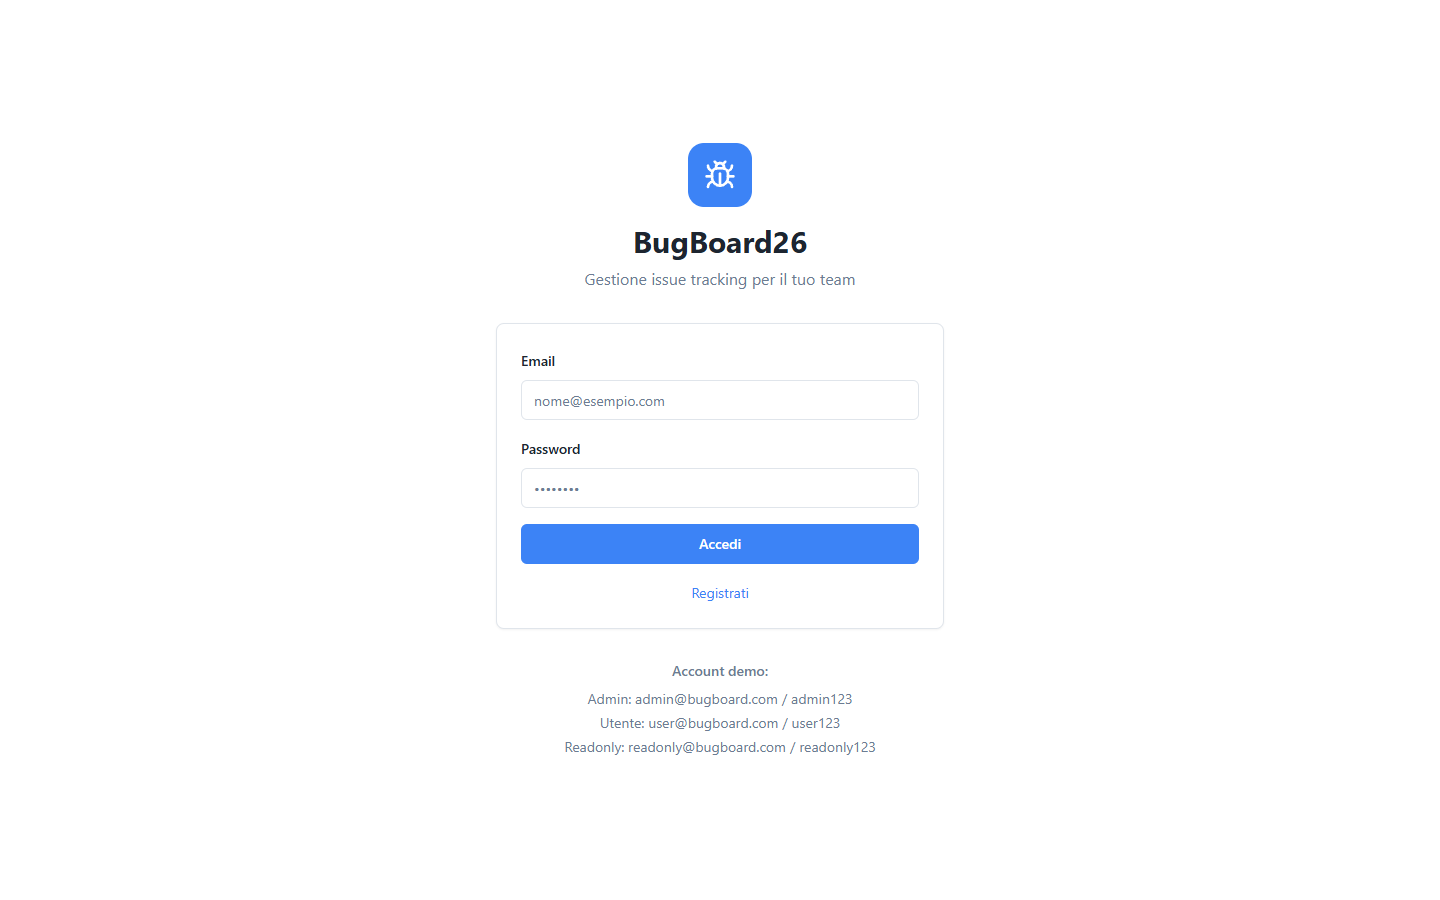
\includegraphics[width=0.85\textwidth]{immagini/mockup_01_login.png}
    \caption{Pagina di Login: form con email e password, pulsante di accesso}
    \label{fig:mockup_login}
\end{figure}

\begin{itemize}
    \item \textbf{Scopo}: autenticazione dell'utente al sistema
    \item \textbf{Elementi}: campo email, campo password, pulsante ``Accedi'', link alla pagina di registrazione
    \item \textbf{Comportamento}: in caso di credenziali errate viene mostrato un messaggio di errore inline; in caso di successo l'utente viene reindirizzato alla Dashboard
\end{itemize}

% ------- 2. REGISTRAZIONE -------
\subsubsection{Mock-up 2 --- Pagina di Registrazione}

\begin{figure}[H]
    \centering
    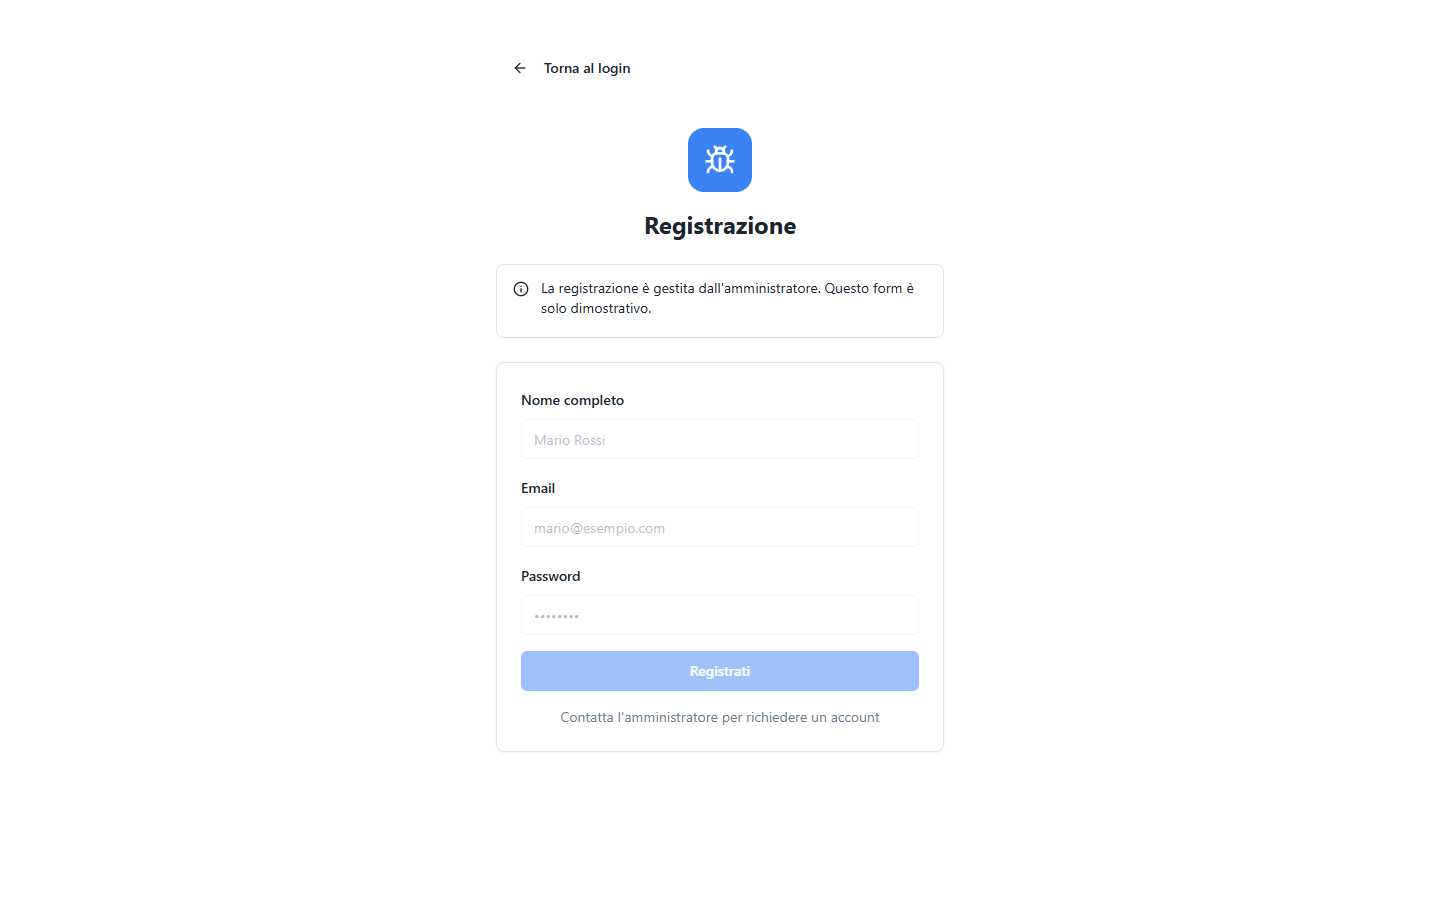
\includegraphics[width=0.85\textwidth]{immagini/mockup_02_register.png}
    \caption{Pagina di Registrazione: form con dati personali e creazione account}
    \label{fig:mockup_register}
\end{figure}

\begin{itemize}
    \item \textbf{Scopo}: creazione di un nuovo account utente
    \item \textbf{Elementi}: campi nome, email, password, conferma password; pulsante ``Registrati''
    \item \textbf{Validazione}: i campi vengono validati in tempo reale con messaggi di errore inline
\end{itemize}

% ------- 3. HOME -------
\subsubsection{Mock-up 3 --- Home / Dashboard}

\begin{figure}[H]
    \centering
    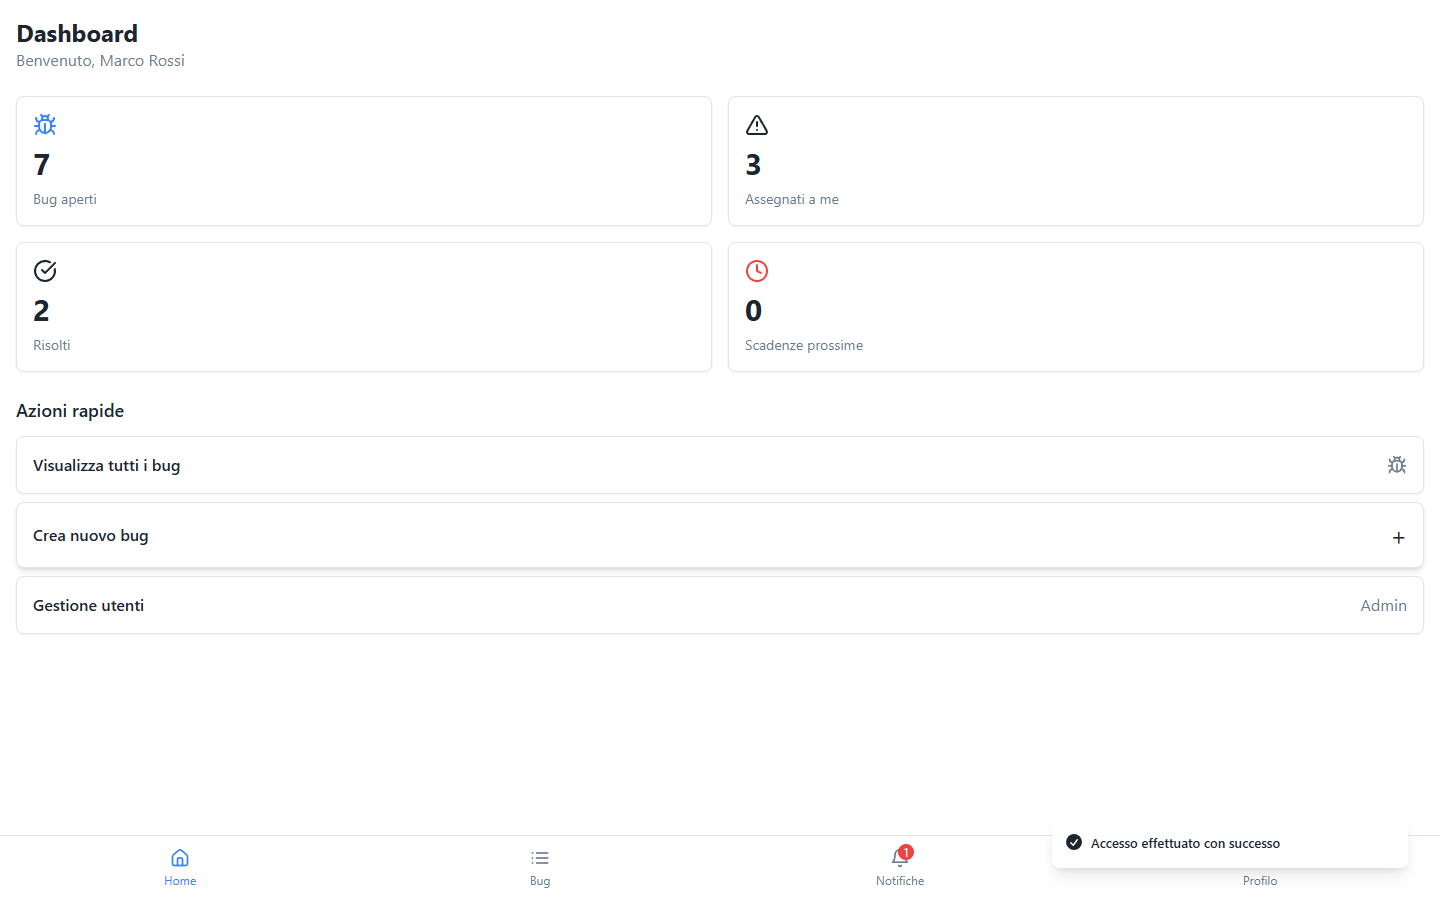
\includegraphics[width=0.85\textwidth]{immagini/mockup_03_home_dashboard.png}
    \caption{Home Dashboard: panoramica delle metriche principali e accessi rapidi}
    \label{fig:mockup_home}
\end{figure}

\begin{itemize}
    \item \textbf{Scopo}: fornire una panoramica immediata dello stato del sistema dopo il login
    \item \textbf{Elementi}: card metriche (bug aperti, assegnati a me, risolti, scadenze prossime), header con navigazione principale
    \item \textbf{Accessi rapidi}: da qui si può navigare alla lista bug, al form di creazione e ai report
\end{itemize}

% ------- 4. LISTA BUG -------
\subsubsection{Mock-up 4 --- Lista Bug con Filtri}

\begin{figure}[H]
    \centering
    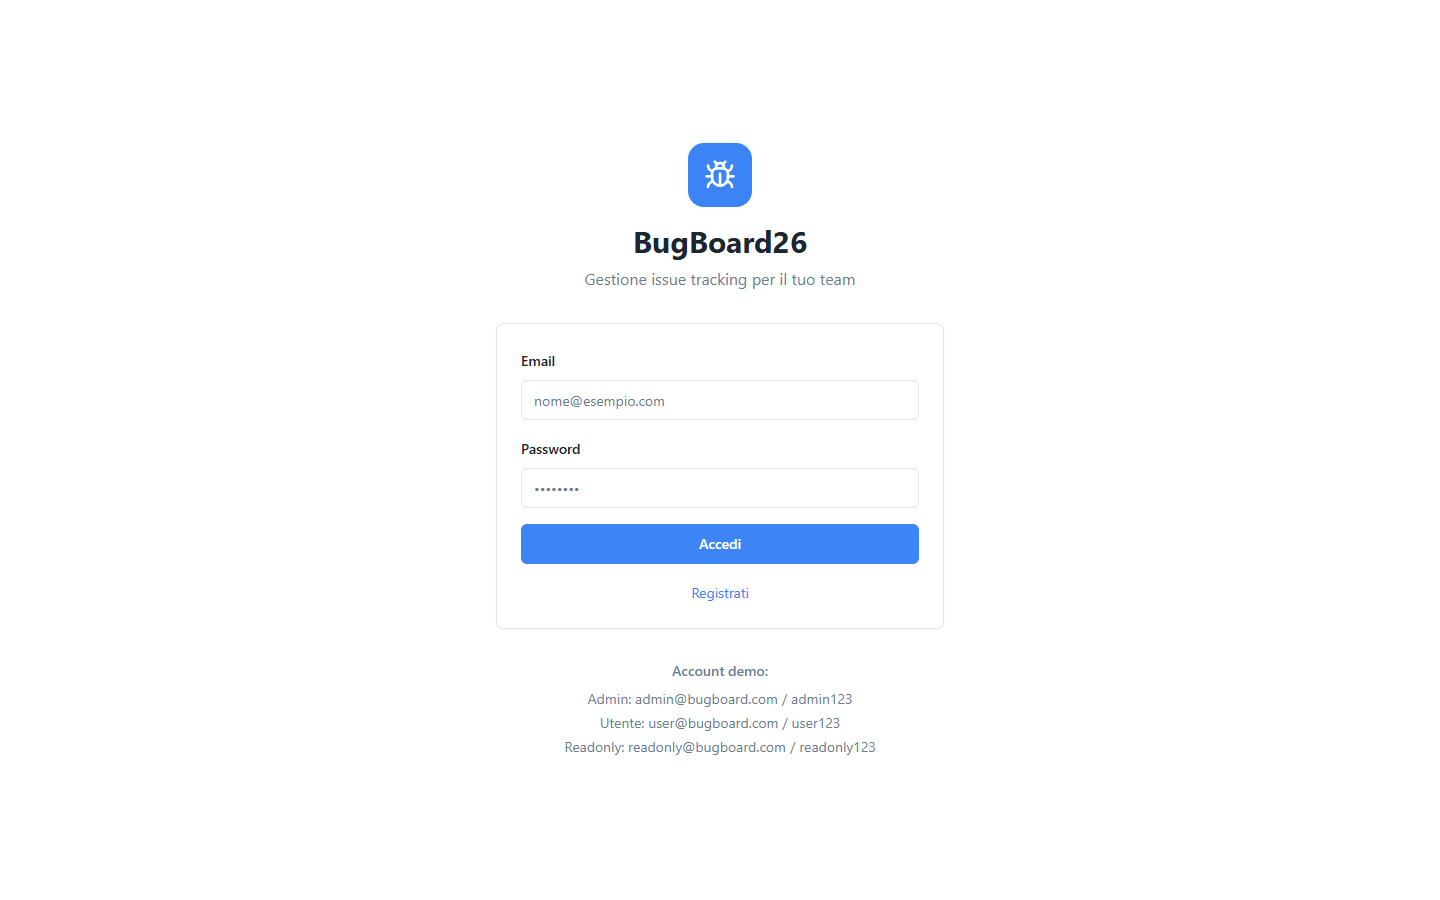
\includegraphics[width=0.85\textwidth]{immagini/mockup_04_lista_bug.png}
    \caption{Lista Bug: tabella con filtri per tipo, stato, priorità e ricerca testuale}
    \label{fig:mockup_lista_bug}
\end{figure}

\begin{itemize}
    \item \textbf{Scopo}: visualizzazione e filtraggio dell'elenco completo dei bug
    \item \textbf{Elementi}: barra filtri orizzontale (tipo, stato, priorità), campo ricerca full-text, tabella bug con badge colorati, paginazione
    \item \textbf{Interazione}: clic su una riga apre il dettaglio del bug; i filtri si applicano in tempo reale
\end{itemize}

% ------- 5. DETTAGLIO BUG -------
\subsubsection{Mock-up 5 --- Dettaglio Bug}

\begin{figure}[H]
    \centering
    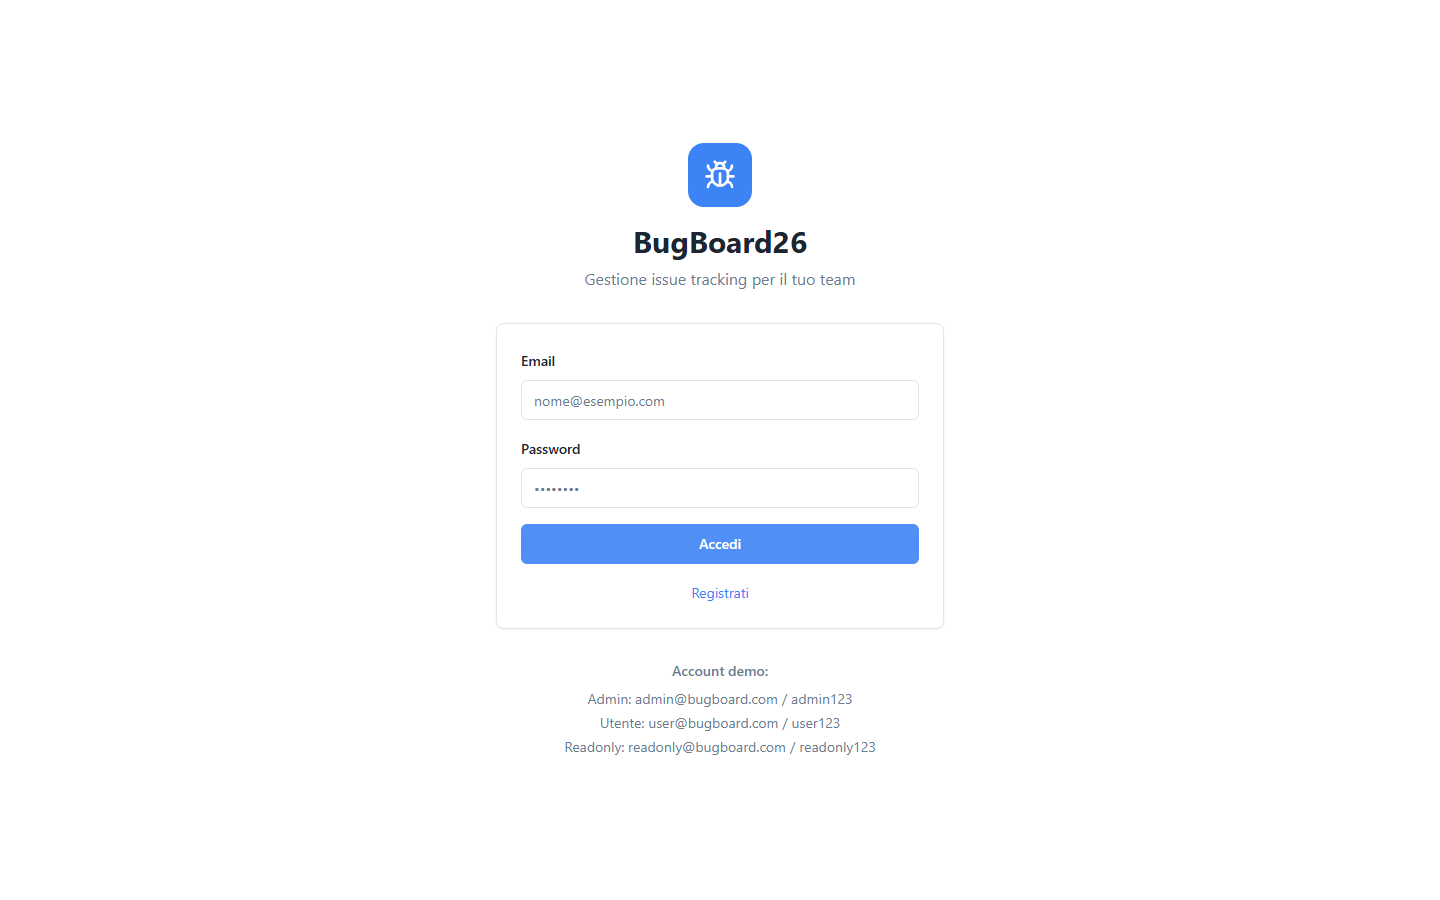
\includegraphics[width=0.85\textwidth]{immagini/mockup_05_dettaglio_bug.png}
    \caption{Dettaglio Bug: informazioni complete, commenti, storico modifiche e azioni disponibili}
    \label{fig:mockup_dettaglio_bug}
\end{figure}

\begin{itemize}
    \item \textbf{Scopo}: visualizzazione completa di un bug specifico e gestione delle azioni disponibili
    \item \textbf{Elementi}: header con titolo, stato e priorità; sezioni descrizione, commenti, allegati, storico; barra azioni laterale (modifica, assegna, risolvi, archivia, duplica)
    \item \textbf{Azioni visibili}: dipendono dal ruolo dell'utente (USER vede meno azioni rispetto ad Admin)
\end{itemize}

% ------- 6. FORM CREAZIONE BUG (UC01) -------
\subsubsection{Mock-up 6 --- Form Creazione/Modifica Bug \textbf{[UC01]}}

\begin{figure}[H]
    \centering
    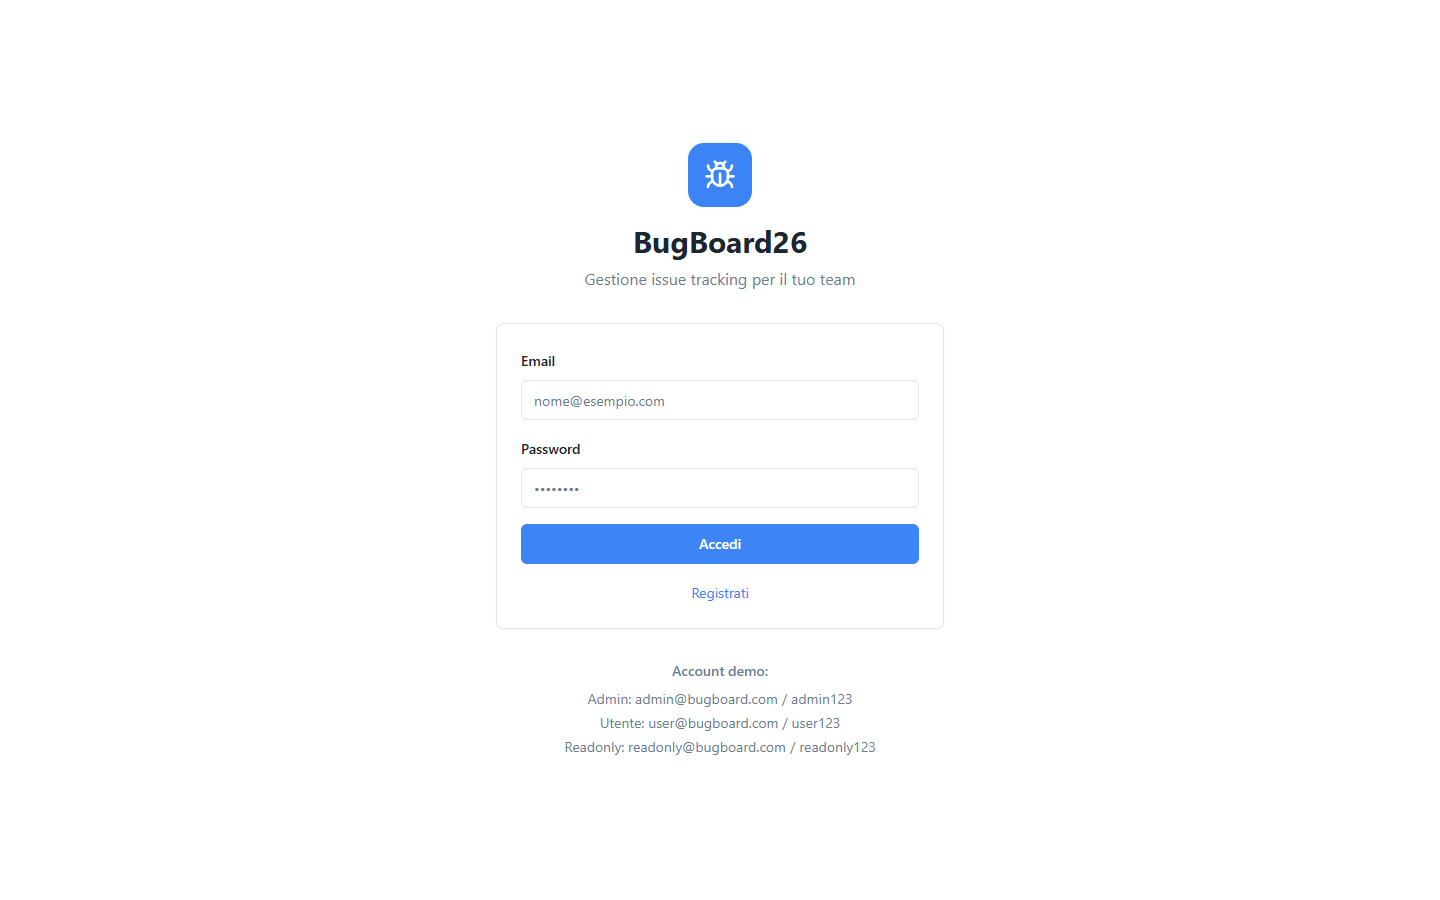
\includegraphics[width=0.85\textwidth]{immagini/mockup_06_form_creazione_bug.png}
    \caption{Form Creazione Bug (UC01): campi titolo, tipo, priorità, descrizione, label, allegati}
    \label{fig:mockup_form_bug}
\end{figure}

\begin{itemize}
    \item \textbf{Caso d'uso}: UC01 --- Creazione nuovo bug
    \item \textbf{Elementi}: campo titolo, selettori tipo e priorità, area di testo descrizione, selezione label multipla, upload allegati immagine, selezione assegnatario opzionale, pulsante ``Salva''
    \item \textbf{Validazione}: i campi obbligatori (titolo, tipo, priorità) sono evidenziati se lasciati vuoti; il formato e la dimensione degli allegati sono verificati prima dell'invio
\end{itemize}

% ------- 7. ASSEGNAZIONE BUG (UC02) -------
\subsubsection{Mock-up 7 --- Assegnazione Bug \textbf{[UC02]}}

\begin{figure}[H]
    \centering
    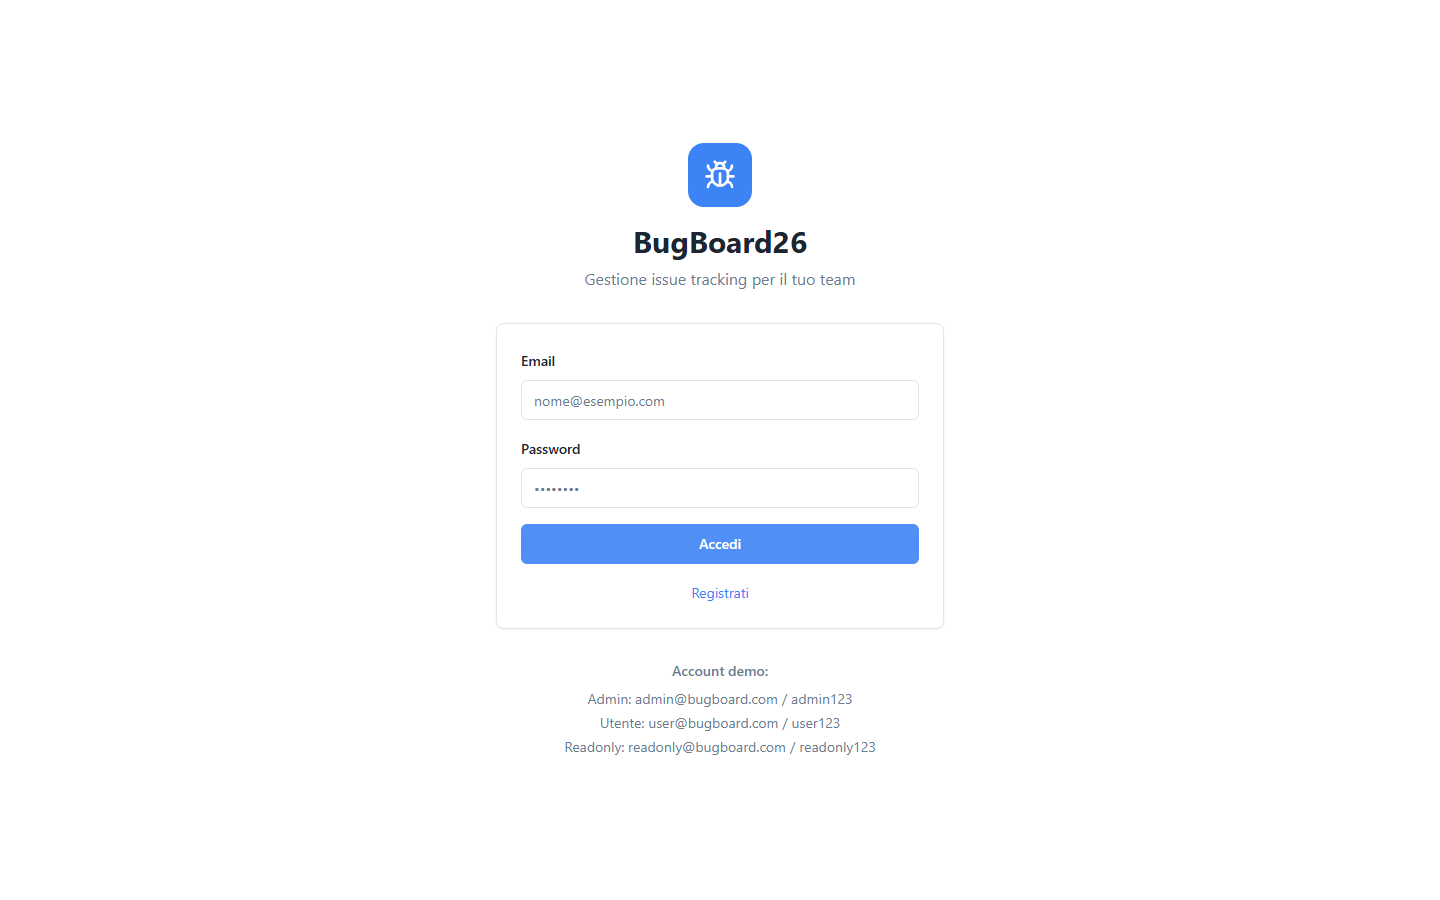
\includegraphics[width=0.85\textwidth]{immagini/mockup_07_assegnazione_bug.png}
    \caption{Assegnazione Bug (UC02): selezione dell'utente a cui assegnare il bug}
    \label{fig:mockup_assegnazione}
\end{figure}

\begin{itemize}
    \item \textbf{Caso d'uso}: UC02 --- Assegnazione bug a un utente (solo Admin)
    \item \textbf{Elementi}: select per la scelta dell'utente assegnatario, pulsante conferma
    \item \textbf{Accesso}: questa schermata è accessibile solo agli utenti con ruolo Admin; un USER viene reindirizzato alla Dashboard
\end{itemize}

% ------- 8. NOTIFICHE -------
\subsubsection{Mock-up 8 --- Notifiche}

\begin{figure}[H]
    \centering
    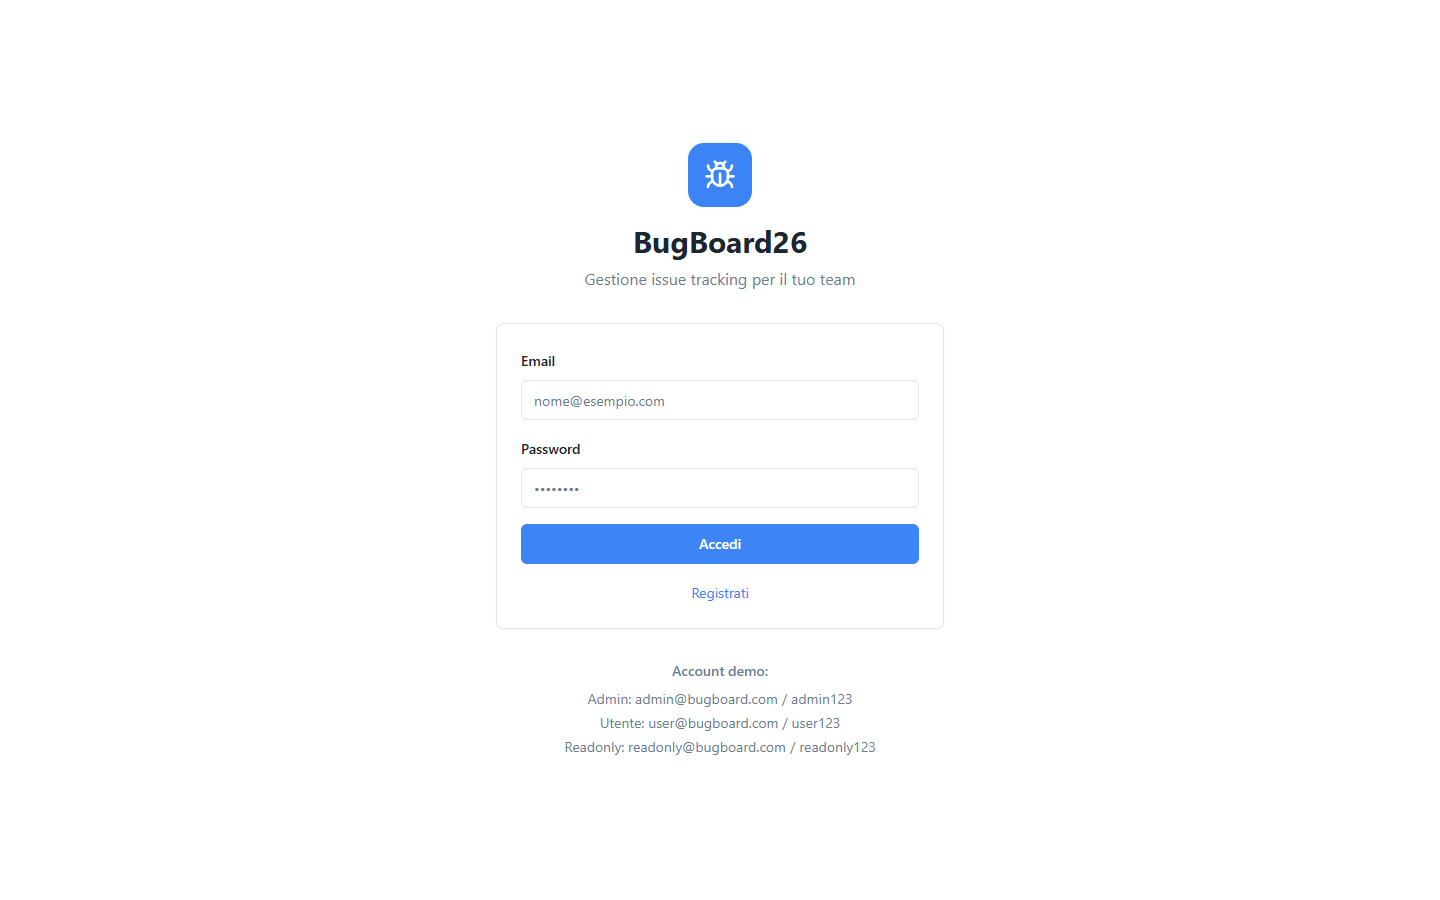
\includegraphics[width=0.85\textwidth]{immagini/mockup_08_notifiche.png}
    \caption{Centro Notifiche: lista degli aggiornamenti sui bug seguiti dall'utente}
    \label{fig:mockup_notifiche}
\end{figure}

\begin{itemize}
    \item \textbf{Scopo}: mostrare all'utente gli aggiornamenti recenti sui bug che lo riguardano (assegnazioni, cambi stato, nuovi commenti)
    \item \textbf{Elementi}: lista notifiche con timestamp, tipo evento e link al bug correlato; indicatore notifiche non lette
\end{itemize}

% ------- 9. PROFILO -------
\subsubsection{Mock-up 9 --- Profilo Utente}

\begin{figure}[H]
    \centering
    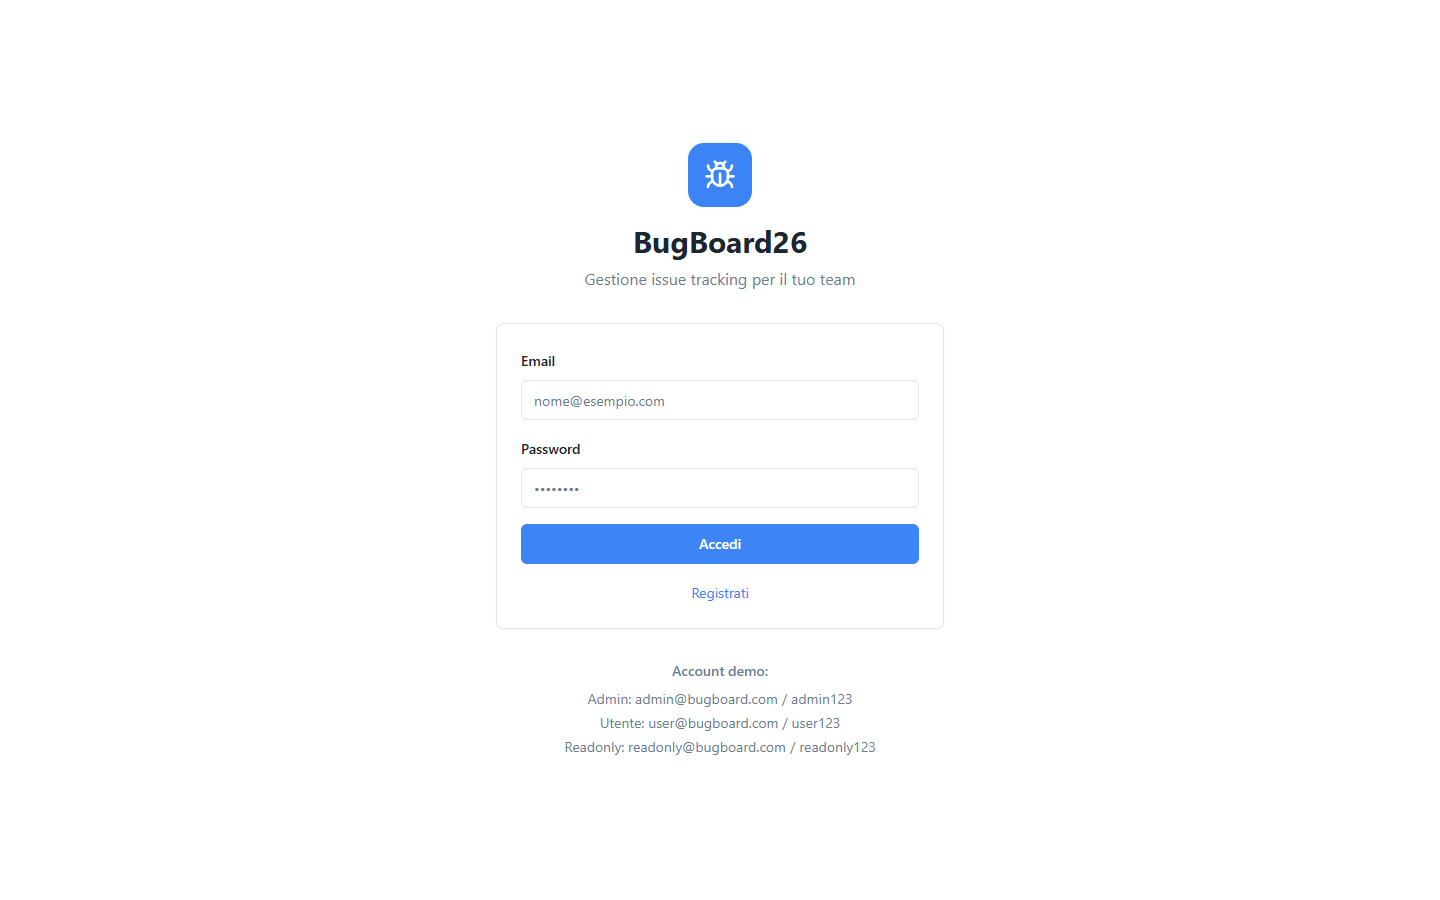
\includegraphics[width=0.85\textwidth]{immagini/mockup_09_profilo.png}
    \caption{Profilo Utente: gestione informazioni personali e cambio password}
    \label{fig:mockup_profilo}
\end{figure}

\begin{itemize}
    \item \textbf{Scopo}: consentire all'utente di visualizzare e modificare le proprie informazioni e la password
    \item \textbf{Elementi}: nome, email, ruolo (in sola lettura), form cambio password con validazione
\end{itemize}

% ------- 10. REPORT MENSILE (UC04) -------
\subsubsection{Mock-up 10 --- Report Mensile \textbf{[UC04]}}

\begin{figure}[H]
    \centering
    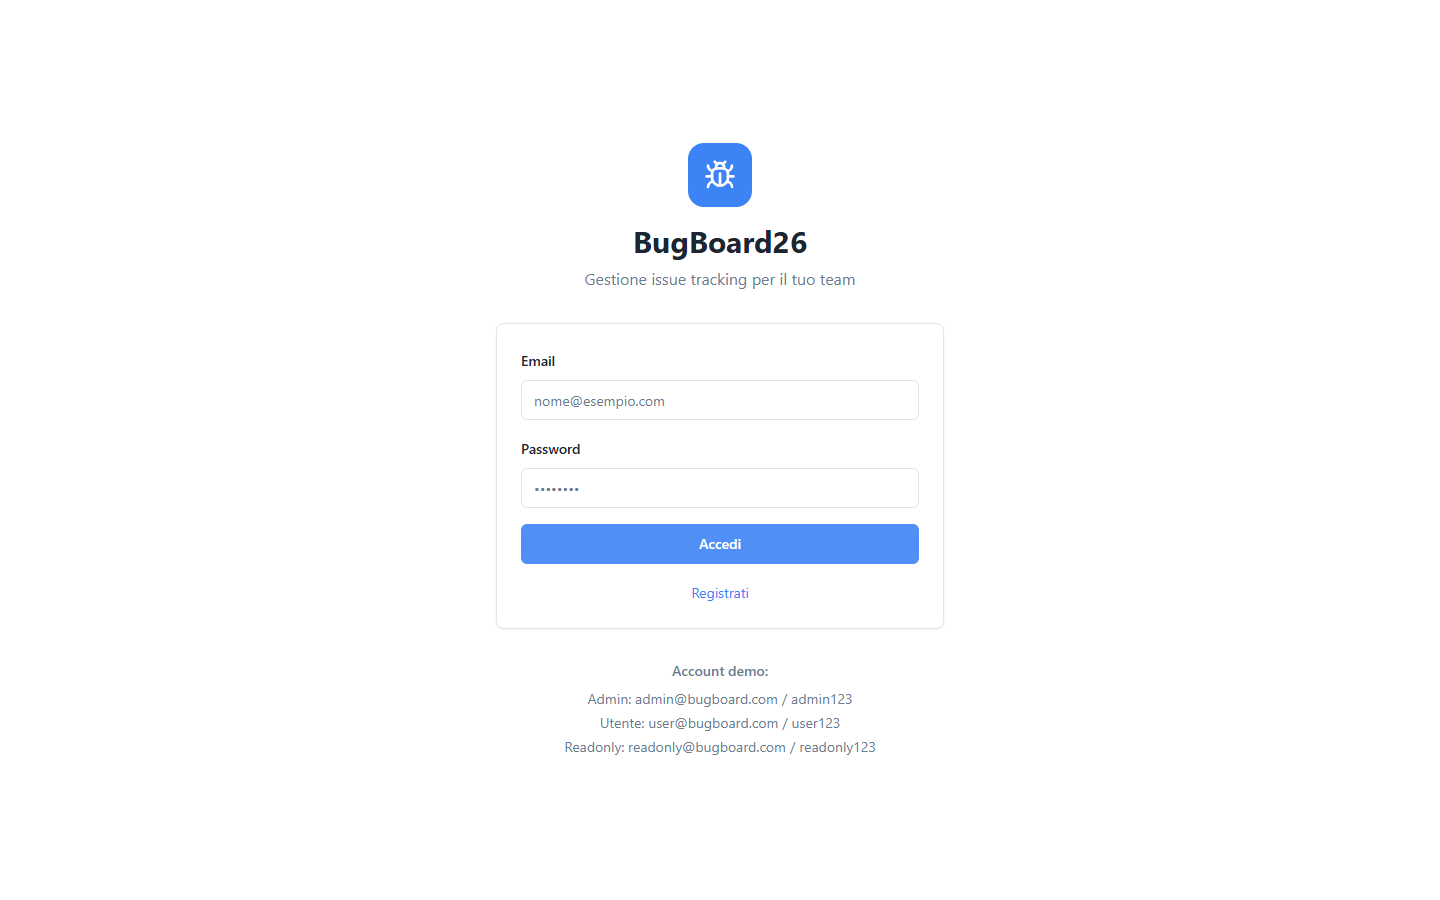
\includegraphics[width=0.85\textwidth]{immagini/mockup_10_report_mensile.png}
    \caption{Report Mensile Admin (UC04): statistiche, grafici e pulsante di export Excel}
    \label{fig:mockup_report}
\end{figure}

\begin{itemize}
    \item \textbf{Caso d'uso}: UC04 --- Generazione report mensile (solo Admin)
    \item \textbf{Elementi}: selettore mese/anno, grafici (distribuzione stato, priorità, trend temporale), tabella riassuntiva metriche, pulsante ``Esporta Excel''
    \item \textbf{Accesso}: solo Admin; gli altri utenti vengono reindirizzati alla Dashboard
\end{itemize}

% ------- 11. GESTIONE UTENTI ADMIN -------
\subsubsection{Mock-up 11 --- Gestione Utenti (Admin)}

\begin{figure}[H]
    \centering
    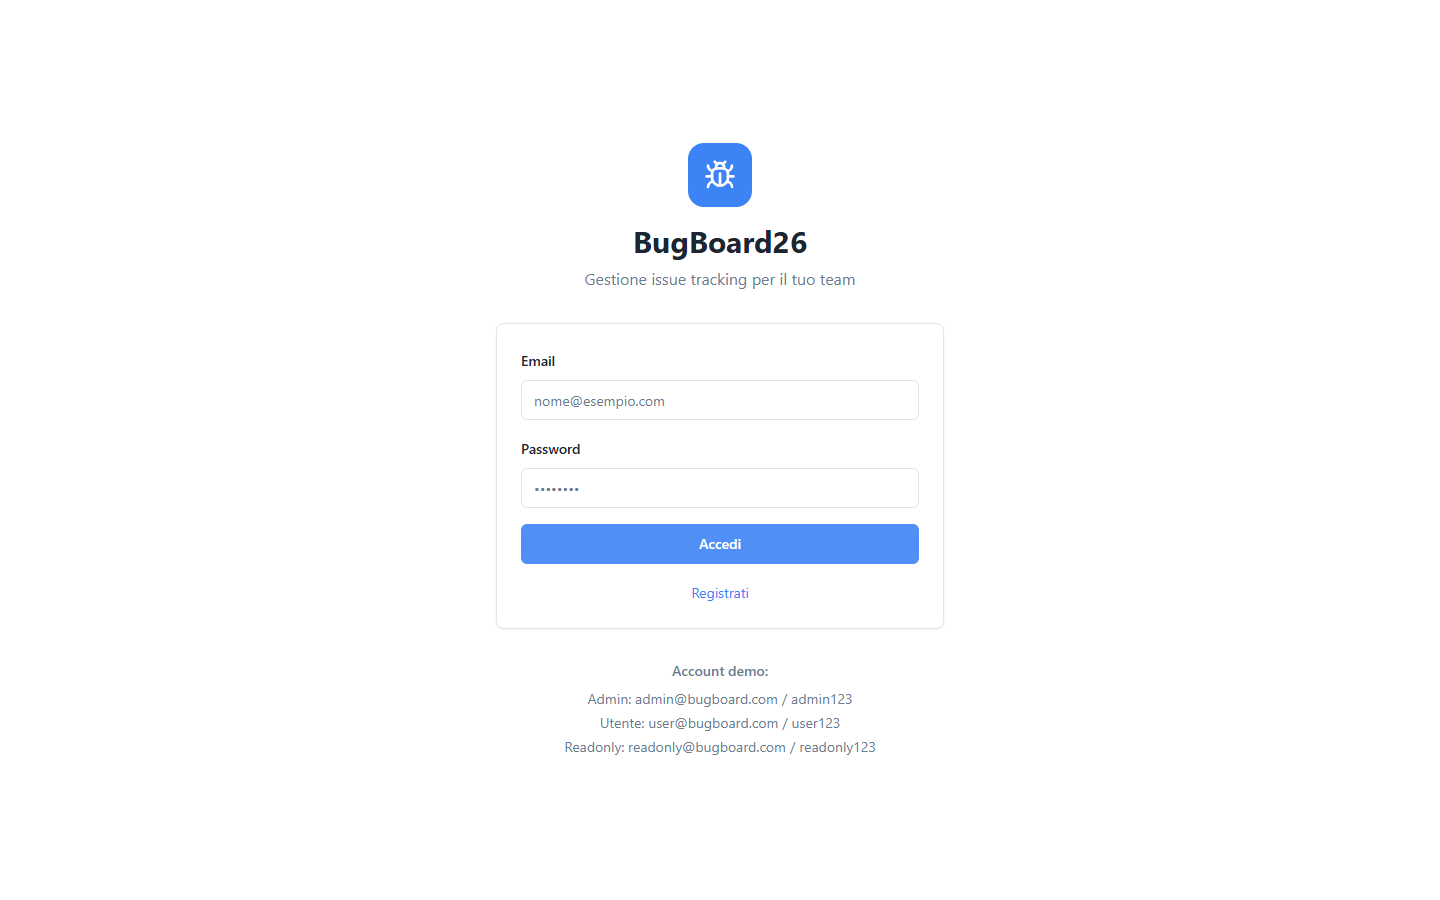
\includegraphics[width=0.85\textwidth]{immagini/mockup_11_admin_utenti.png}
    \caption{Gestione Utenti Admin: lista utenti con ruoli, stato e azioni di modifica}
    \label{fig:mockup_admin_utenti}
\end{figure}

\begin{itemize}
    \item \textbf{Scopo}: permettere all'Admin di gestire gli account del sistema (visualizzazione ruoli, disabilitazione utenti)
    \item \textbf{Elementi}: tabella utenti con email, nome, ruolo e stato; azioni per modifica ruolo e disabilitazione account
\end{itemize}

% ------- 12. ARCHIVIO -------
\subsubsection{Mock-up 12 --- Archivio Bug}

\begin{figure}[H]
    \centering
    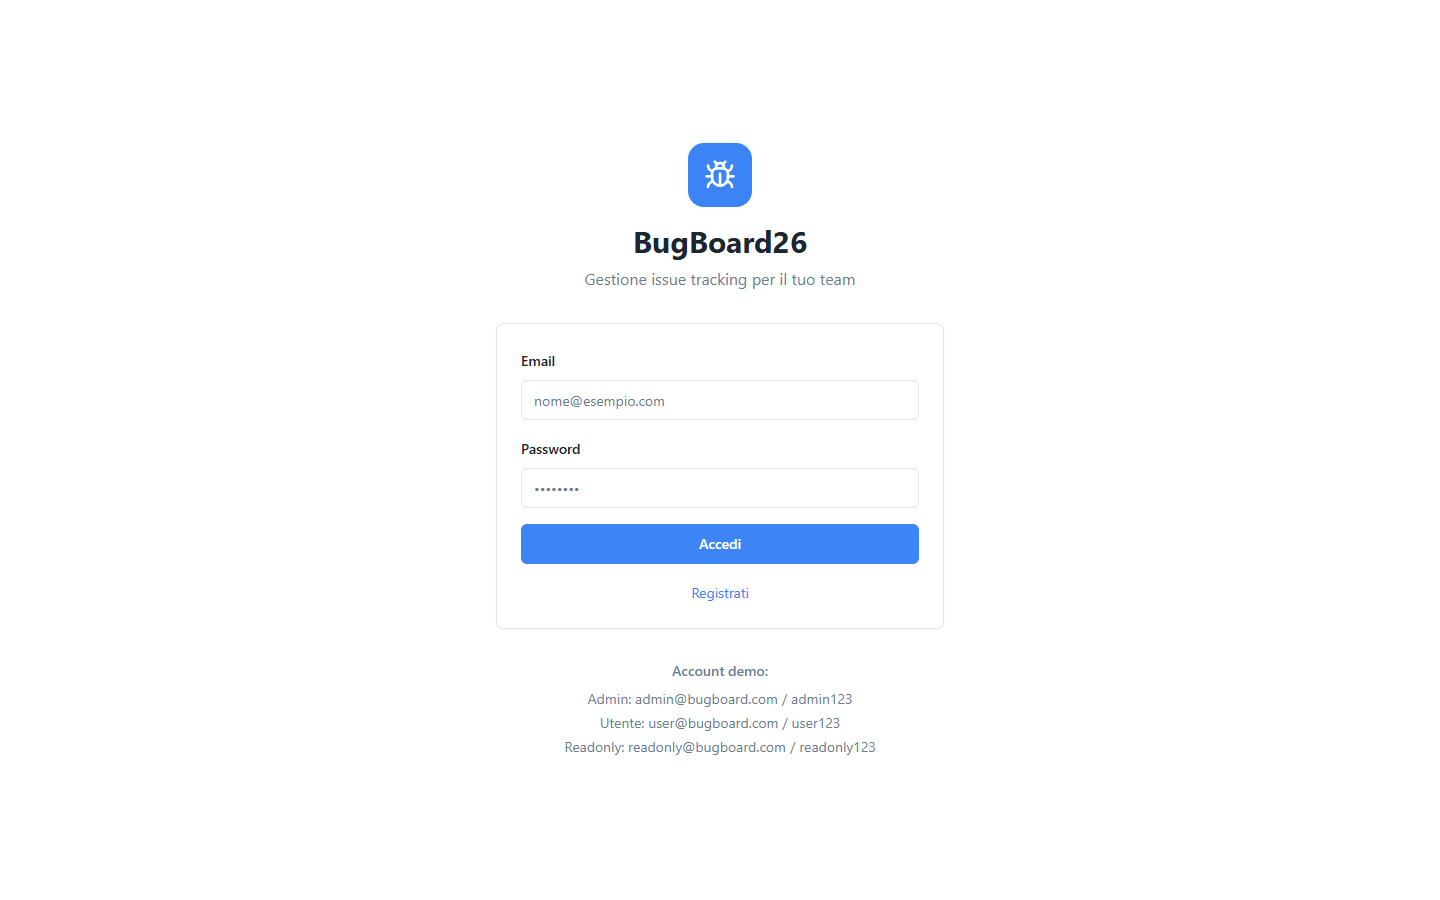
\includegraphics[width=0.85\textwidth]{immagini/mockup_12_archivio.png}
    \caption{Archivio Bug: lista dei bug archiviati con possibilità di consultazione}
    \label{fig:mockup_archivio}
\end{figure}

\begin{itemize}
    \item \textbf{Scopo}: visualizzare i bug archiviati per storico e consultazione senza influire sulla lista attiva
    \item \textbf{Elementi}: tabella bug in stato \textit{Archived} con filtri e ricerca; solo Admin può archiviare/ripristinare bug
\end{itemize}

% ------- 13. EXPORT -------
\subsubsection{Mock-up 13 --- Export Dati}

\begin{figure}[H]
    \centering
    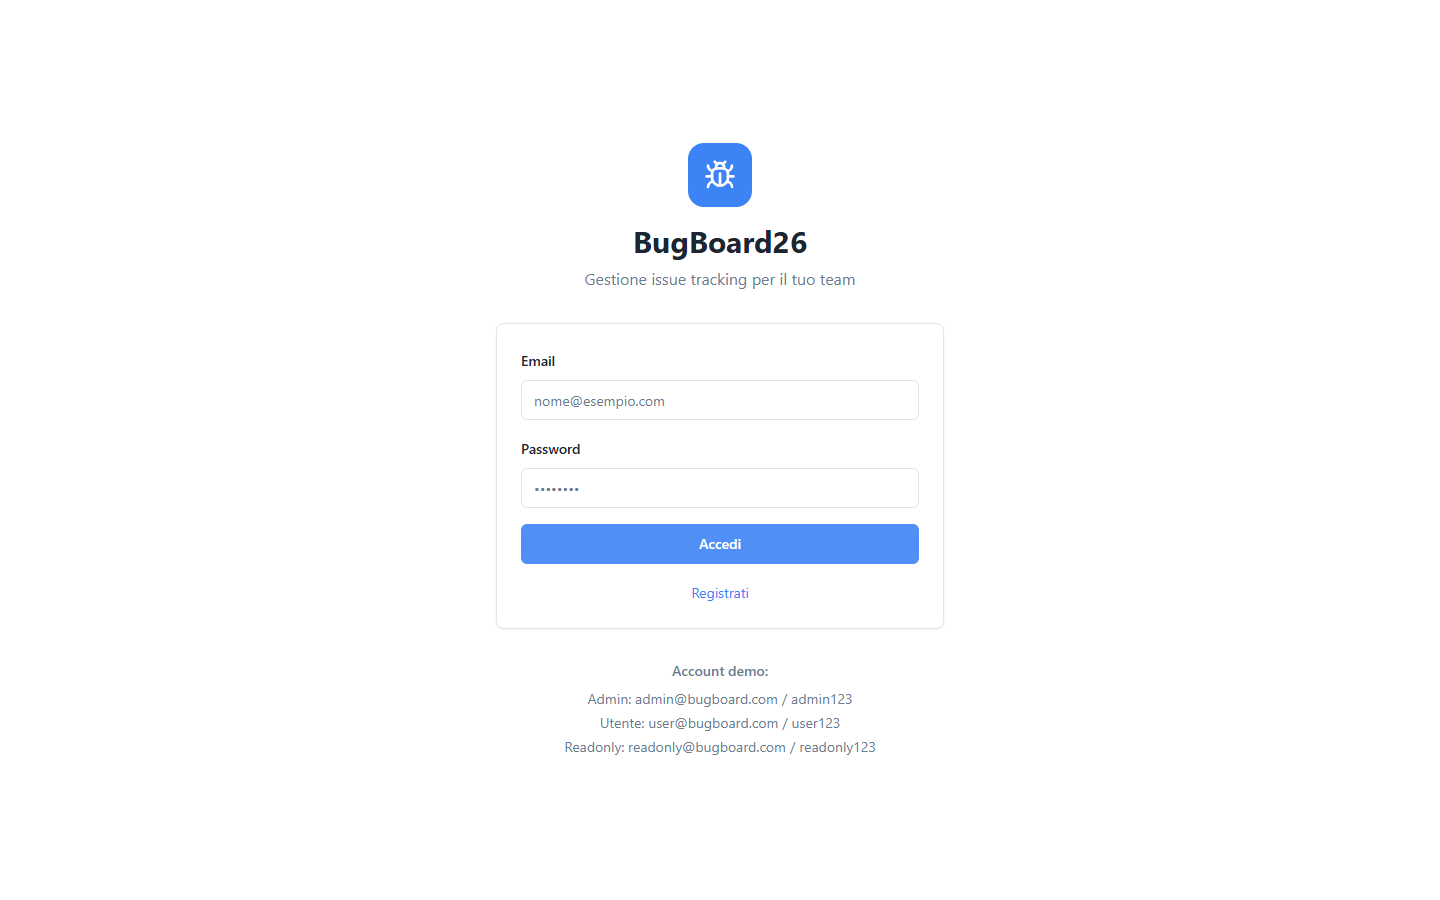
\includegraphics[width=0.85\textwidth]{immagini/mockup_13_export.png}
    \caption{Export Dati: download dell'elenco bug in formato CSV o Excel}
    \label{fig:mockup_export}
\end{figure}

\begin{itemize}
    \item \textbf{Scopo}: consentire l'esportazione dei dati per analisi esterne
    \item \textbf{Elementi}: pulsanti ``Scarica CSV'' e ``Scarica Excel''; i file vengono generati dal backend e scaricati direttamente
\end{itemize}

% ------------------------------------------------------------
\subsection{Osservazioni emerse dalla prototipazione}

La realizzazione del prototipo funzionante ha permesso di identificare alcune scelte migliorative rispetto all'analisi iniziale:

\begin{itemize}
    \item \textbf{Chiarezza dei ruoli}: è stato necessario rendere esplicito nel UI quali azioni sono riservate all'Admin (assegnazione, report, archiviazione, gestione utenti), aggiungendo reindirizzamenti automatici per utenti non autorizzati
    \item \textbf{Filtri immediati}: la lista bug con filtri in tempo reale si è rivelata la funzionalità più usata nelle sessioni di test, confermando la scelta di renderla la pagina principale
    \item \textbf{Badge colorati}: l'uso di badge cromatici per stato, priorità e tipo ha migliorato significativamente la leggibilità della lista bug senza aprire il dettaglio
    \item \textbf{Navigazione mobile}: il menu hamburger con le stesse voci del desktop ha garantito piena parità funzionale su dispositivi mobili
\end{itemize}

% ============================================================

\section{Prototipazione visuale attraverso Mock-up}

La prototipazione visuale di BugBoard26 è stata realizzata direttamente come applicazione React funzionante, con dati simulati (\textit{mock data}). Le schermate qui mostrate sono catture reali del prototipo interattivo, e non semplici bozzetti grafici. Questo approccio ha permesso di validare il flusso utente in modo concreto fin dalla fase di analisi.

% ------------------------------------------------------------
\subsection{Scelte Progettuali}

\subsubsection{Layout e Navigazione}
\begin{itemize}
    \item \textbf{Header fisso}: barra superiore con logo, link alle sezioni principali (Dashboard, Bug, Report, Admin) e menu utente con avatar, email e pulsante logout
    \item \textbf{Navigazione mobile}: menu a comparsa (hamburger) con le stesse voci, ottimizzato per touch
    \item \textbf{Layout responsive}: design \textit{mobile-first} realizzato con Tailwind CSS; le griglie si adattano automaticamente a qualsiasi larghezza schermo
\end{itemize}

\subsubsection{Palette Colori e Badge}
\begin{itemize}
    \item \textbf{Priorità}: \textit{Critical} (rosso), \textit{High} (arancione), \textit{Medium} (giallo), \textit{Low} (verde)
    \item \textbf{Stato}: \textit{Todo} (grigio chiaro), \textit{In Progress} (blu), \textit{Resolved} (verde), \textit{Archived} (grigio scuro)
    \item \textbf{Tipo}: \textit{Bug} (rosso), \textit{Feature} (viola), \textit{Enhancement} (azzurro)
    \item \textbf{Azioni primarie}: blu (\texttt{\#007BFF}); superfici neutre: grigi Tailwind
\end{itemize}

\subsubsection{Componenti UI riutilizzati}
Tutti i componenti sono basati su \textbf{Radix UI} e \textbf{shadcn/ui}: Button, Card, Select, Dialog, Badge, Table, Toast, DropdownMenu. Questo garantisce coerenza visiva e accessibilità WCAG 2.1 out-of-the-box.

% ------------------------------------------------------------
\subsection{Mock-up delle interfacce utente}

Di seguito sono illustrate le schermate principali del prototipo, raggruppate per funzionalità. Le schermate contrassegnate con \textbf{[UC0X]} corrispondono direttamente ai casi d'uso formalizzati nella sezione precedente.

% ------- 1. LOGIN -------
\subsubsection{Mock-up 1 --- Pagina di Login}

\begin{figure}[H]
    \centering
    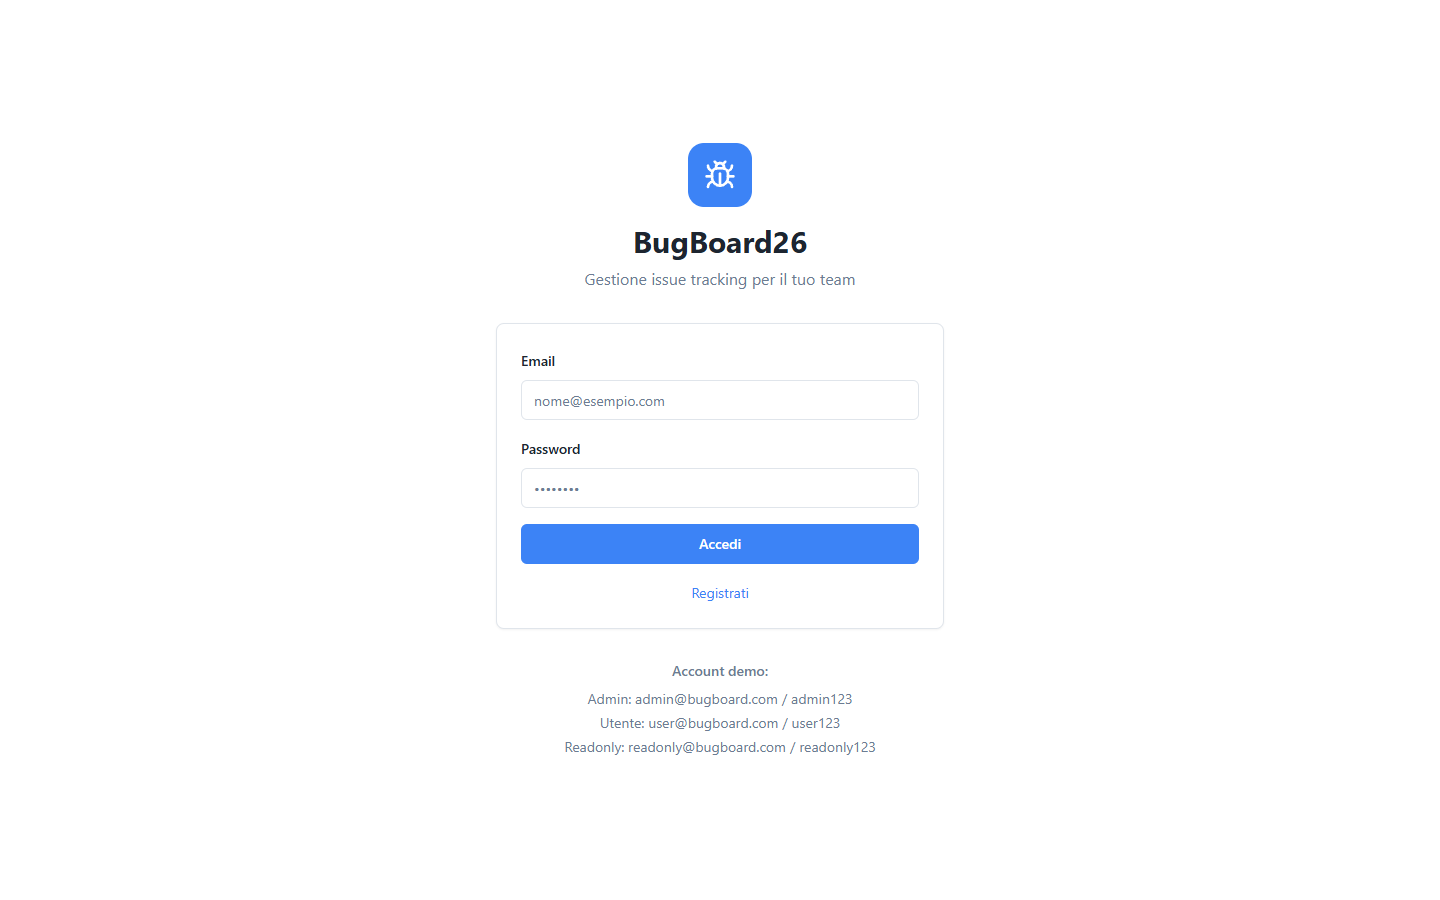
\includegraphics[width=0.85\textwidth]{immagini/mockup_01_login.png}
    \caption{Pagina di Login: form con email e password, pulsante di accesso}
    \label{fig:mockup_login}
\end{figure}

\begin{itemize}
    \item \textbf{Scopo}: autenticazione dell'utente al sistema
    \item \textbf{Elementi}: campo email, campo password, pulsante ``Accedi'', link alla pagina di registrazione
    \item \textbf{Comportamento}: in caso di credenziali errate viene mostrato un messaggio di errore inline; in caso di successo l'utente viene reindirizzato alla Dashboard
\end{itemize}

% ------- 2. REGISTRAZIONE -------
\subsubsection{Mock-up 2 --- Pagina di Registrazione}

\begin{figure}[H]
    \centering
    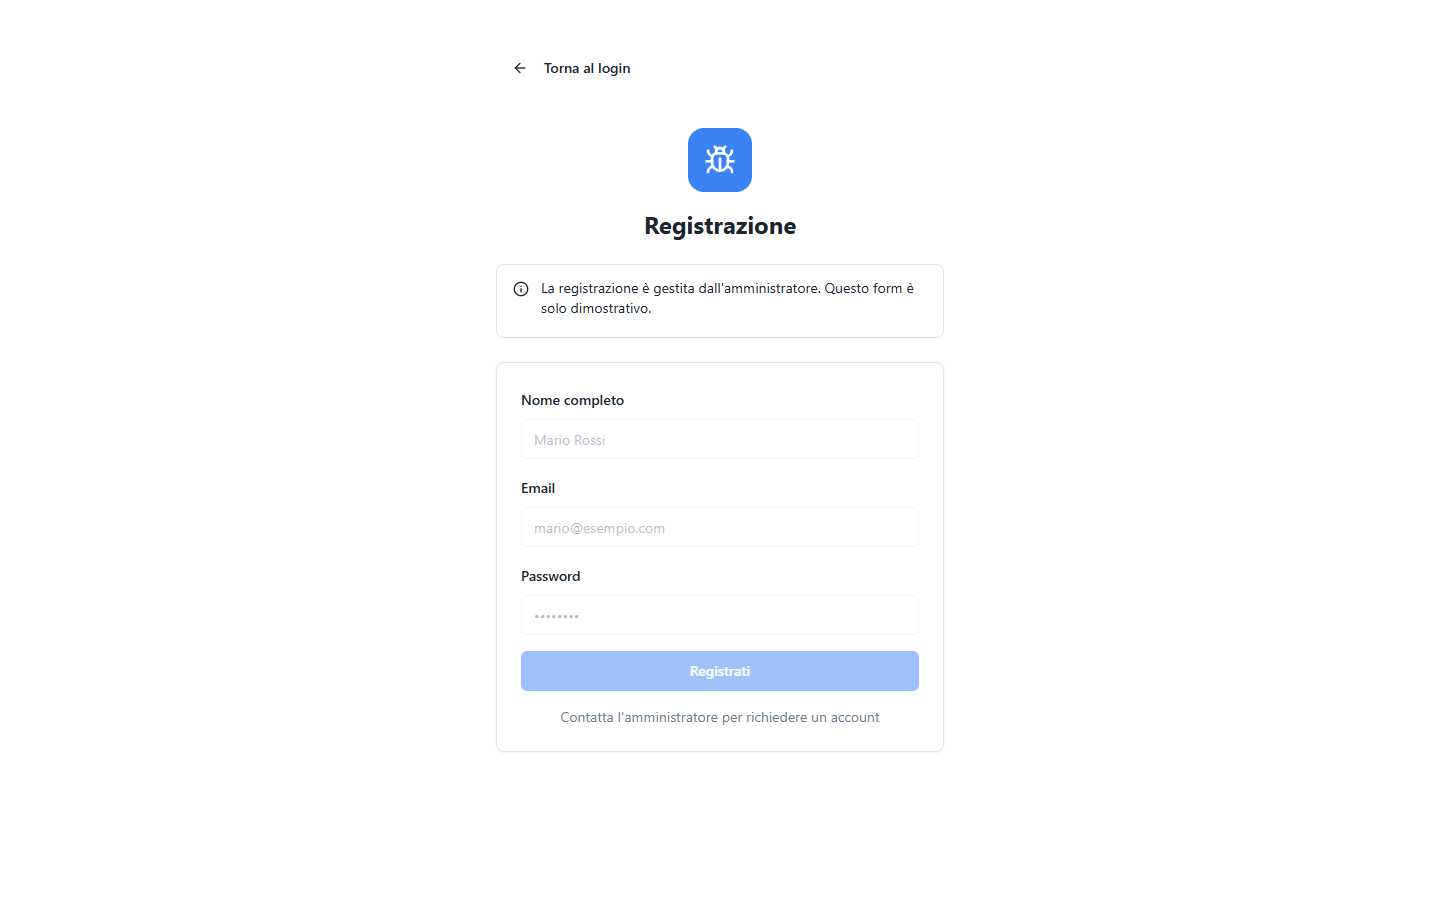
\includegraphics[width=0.85\textwidth]{immagini/mockup_02_register.png}
    \caption{Pagina di Registrazione: form con dati personali e creazione account}
    \label{fig:mockup_register}
\end{figure}

\begin{itemize}
    \item \textbf{Scopo}: creazione di un nuovo account utente
    \item \textbf{Elementi}: campi nome, email, password, conferma password; pulsante ``Registrati''
    \item \textbf{Validazione}: i campi vengono validati in tempo reale con messaggi di errore inline
\end{itemize}

% ------- 3. HOME -------
\subsubsection{Mock-up 3 --- Home / Dashboard}

\begin{figure}[H]
    \centering
    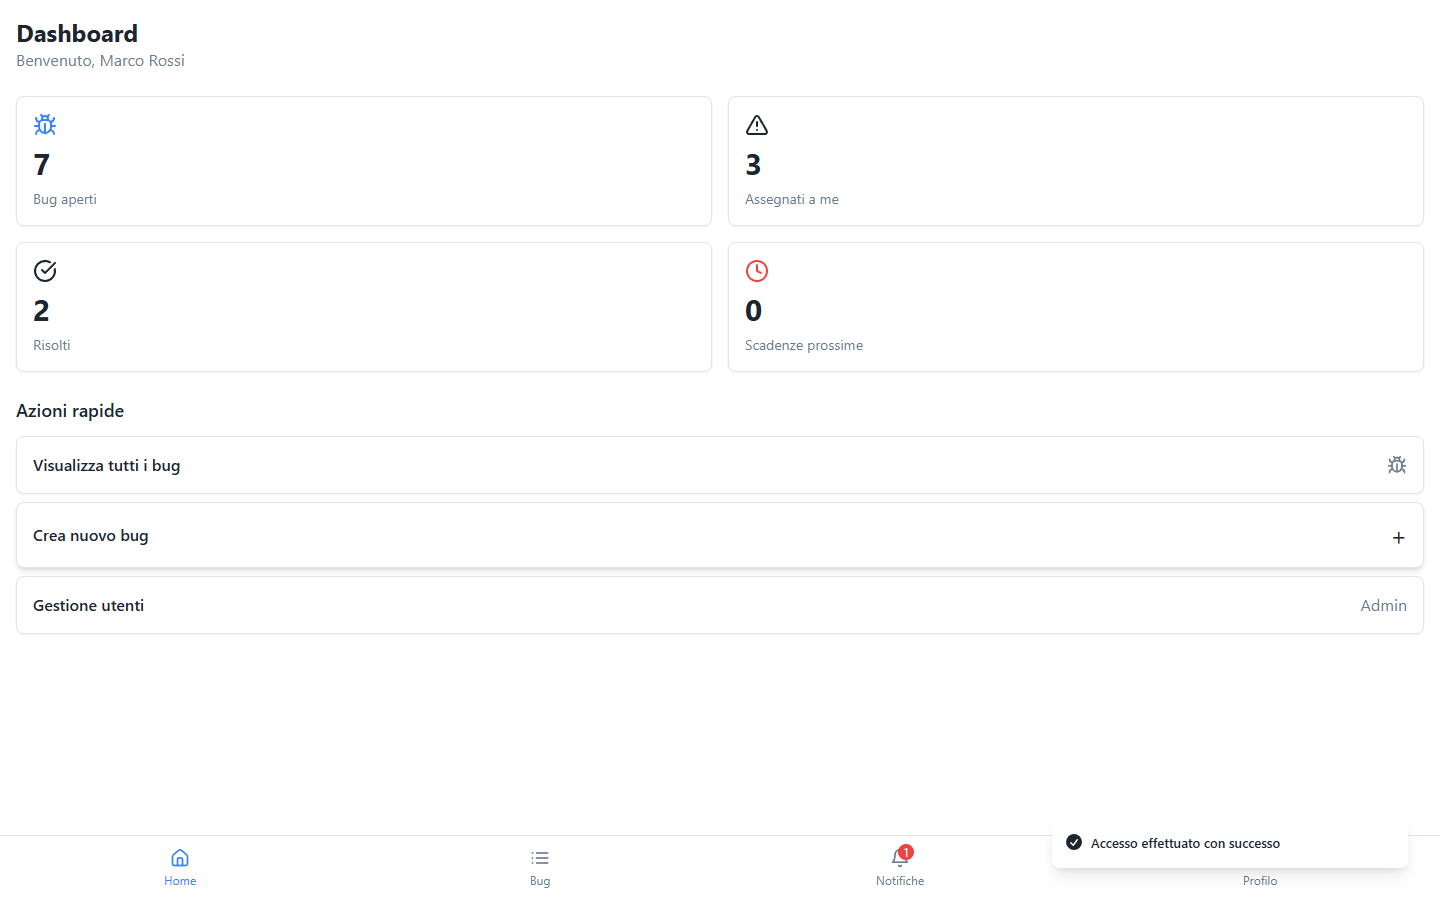
\includegraphics[width=0.85\textwidth]{immagini/mockup_03_home_dashboard.png}
    \caption{Home Dashboard: panoramica delle metriche principali e accessi rapidi}
    \label{fig:mockup_home}
\end{figure}

\begin{itemize}
    \item \textbf{Scopo}: fornire una panoramica immediata dello stato del sistema dopo il login
    \item \textbf{Elementi}: card metriche (bug aperti, assegnati a me, risolti, scadenze prossime), header con navigazione principale
    \item \textbf{Accessi rapidi}: da qui si può navigare alla lista bug, al form di creazione e ai report
\end{itemize}

% ------- 4. LISTA BUG -------
\subsubsection{Mock-up 4 --- Lista Bug con Filtri}

\begin{figure}[H]
    \centering
    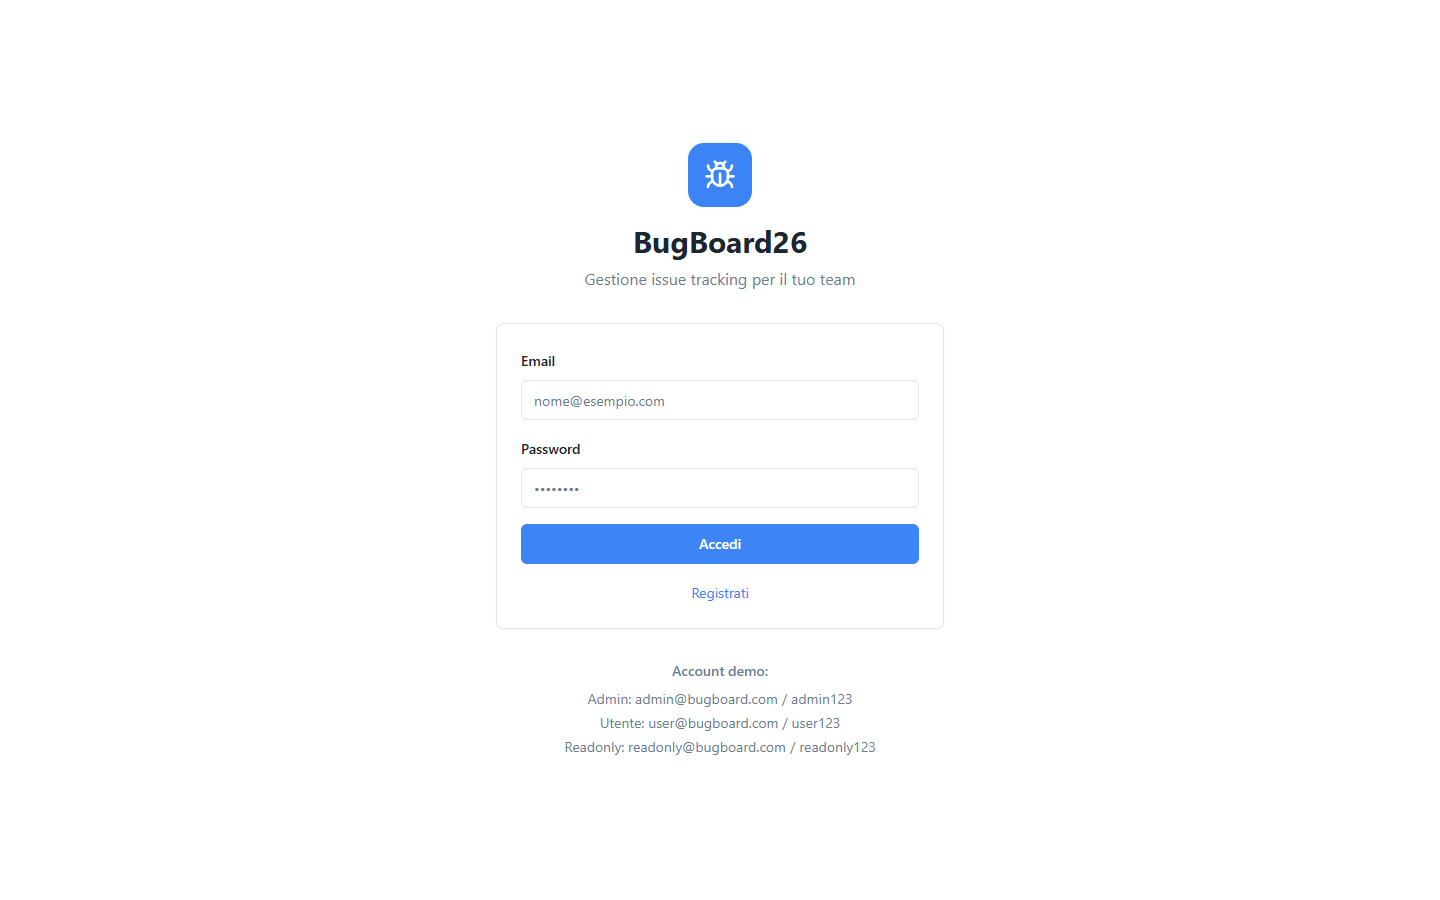
\includegraphics[width=0.85\textwidth]{immagini/mockup_04_lista_bug.png}
    \caption{Lista Bug: tabella con filtri per tipo, stato, priorità e ricerca testuale}
    \label{fig:mockup_lista_bug}
\end{figure}

\begin{itemize}
    \item \textbf{Scopo}: visualizzazione e filtraggio dell'elenco completo dei bug
    \item \textbf{Elementi}: barra filtri orizzontale (tipo, stato, priorità), campo ricerca full-text, tabella bug con badge colorati, paginazione
    \item \textbf{Interazione}: clic su una riga apre il dettaglio del bug; i filtri si applicano in tempo reale
\end{itemize}

% ------- 5. DETTAGLIO BUG -------
\subsubsection{Mock-up 5 --- Dettaglio Bug}

\begin{figure}[H]
    \centering
    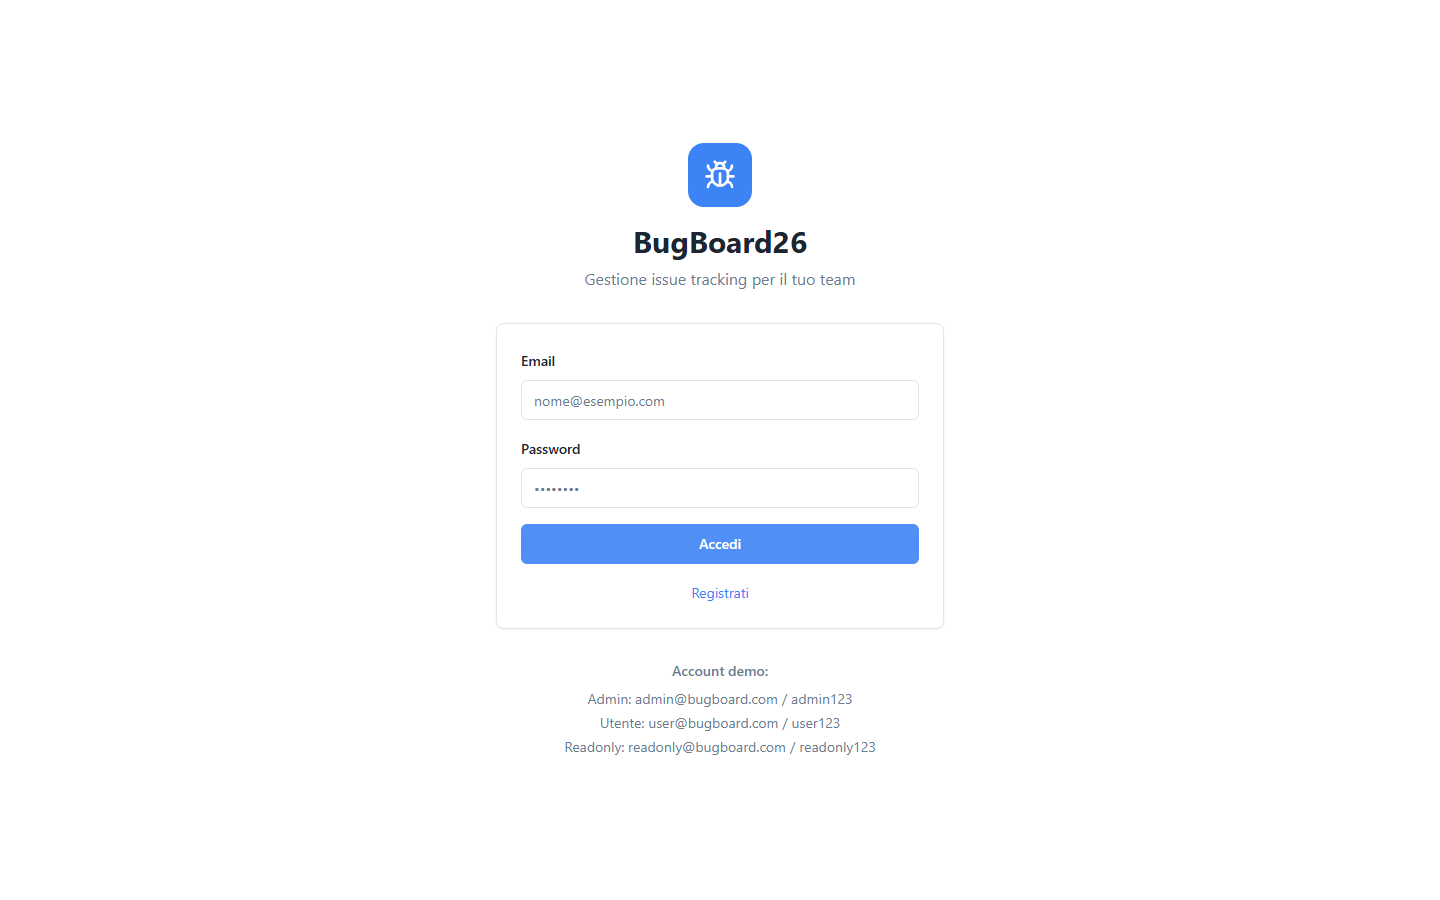
\includegraphics[width=0.85\textwidth]{immagini/mockup_05_dettaglio_bug.png}
    \caption{Dettaglio Bug: informazioni complete, commenti, storico modifiche e azioni disponibili}
    \label{fig:mockup_dettaglio_bug}
\end{figure}

\begin{itemize}
    \item \textbf{Scopo}: visualizzazione completa di un bug specifico e gestione delle azioni disponibili
    \item \textbf{Elementi}: header con titolo, stato e priorità; sezioni descrizione, commenti, allegati, storico; barra azioni laterale (modifica, assegna, risolvi, archivia, duplica)
    \item \textbf{Azioni visibili}: dipendono dal ruolo dell'utente (USER vede meno azioni rispetto ad Admin)
\end{itemize}

% ------- 6. FORM CREAZIONE BUG (UC01) -------
\subsubsection{Mock-up 6 --- Form Creazione/Modifica Bug \textbf{[UC01]}}

\begin{figure}[H]
    \centering
    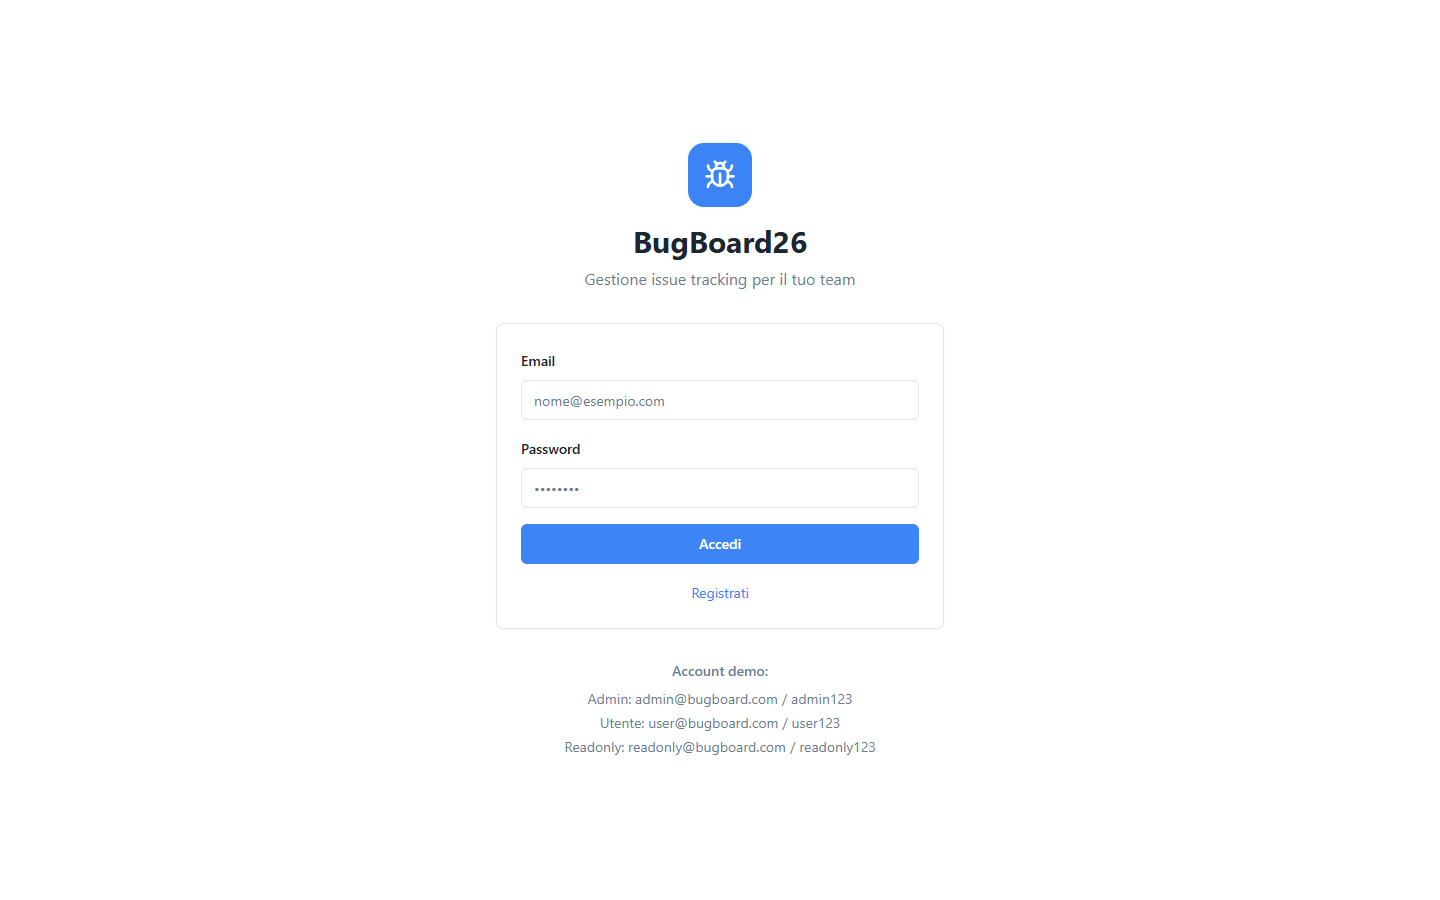
\includegraphics[width=0.85\textwidth]{immagini/mockup_06_form_creazione_bug.png}
    \caption{Form Creazione Bug (UC01): campi titolo, tipo, priorità, descrizione, label, allegati}
    \label{fig:mockup_form_bug}
\end{figure}

\begin{itemize}
    \item \textbf{Caso d'uso}: UC01 --- Creazione nuovo bug
    \item \textbf{Elementi}: campo titolo, selettori tipo e priorità, area di testo descrizione, selezione label multipla, upload allegati immagine, selezione assegnatario opzionale, pulsante ``Salva''
    \item \textbf{Validazione}: i campi obbligatori (titolo, tipo, priorità) sono evidenziati se lasciati vuoti; il formato e la dimensione degli allegati sono verificati prima dell'invio
\end{itemize}

% ------- 7. ASSEGNAZIONE BUG (UC02) -------
\subsubsection{Mock-up 7 --- Assegnazione Bug \textbf{[UC02]}}

\begin{figure}[H]
    \centering
    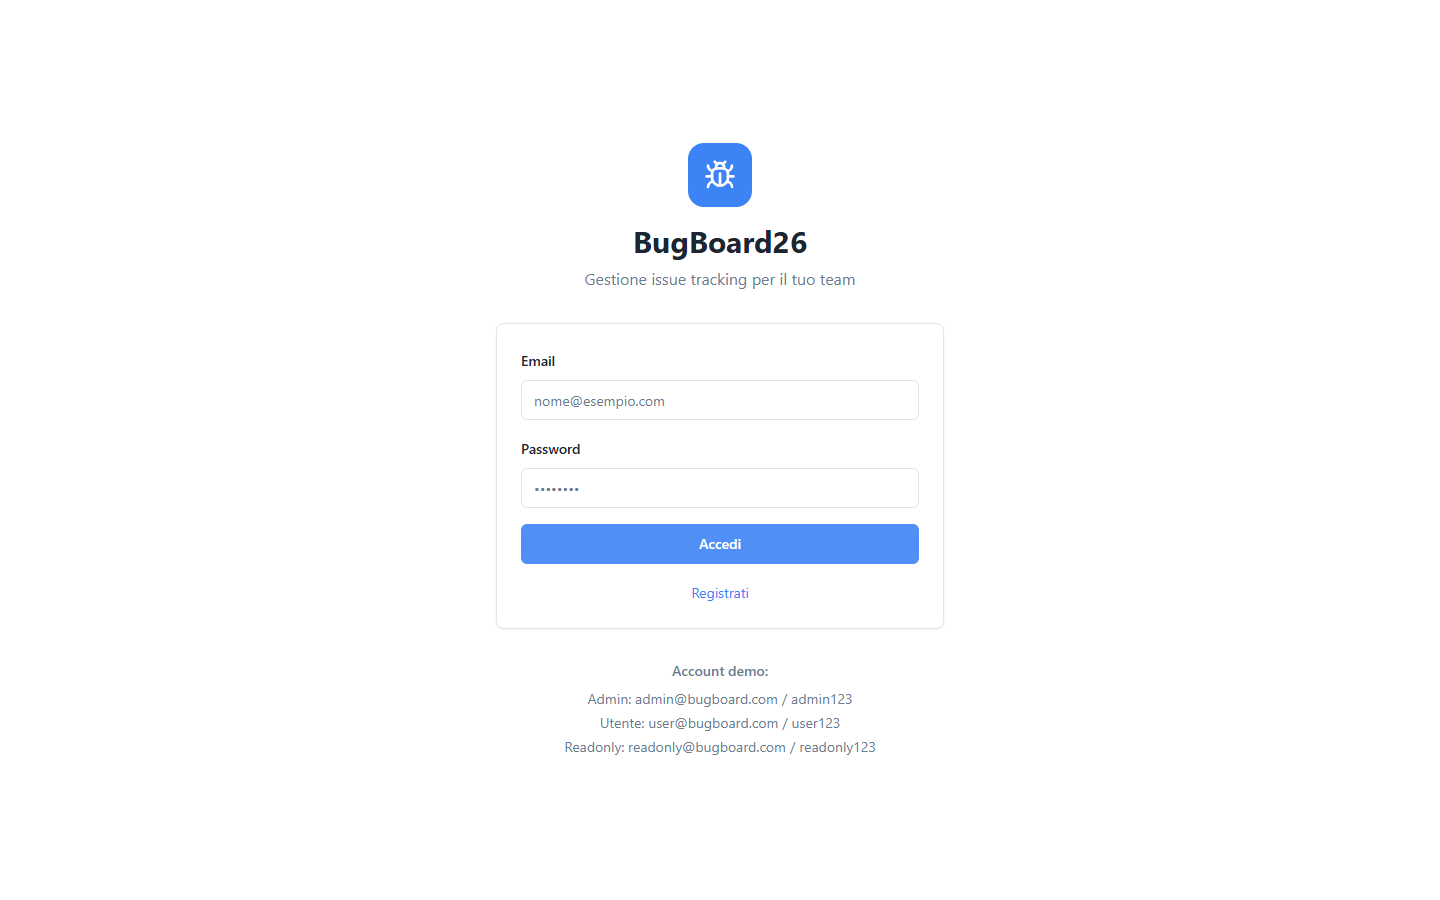
\includegraphics[width=0.85\textwidth]{immagini/mockup_07_assegnazione_bug.png}
    \caption{Assegnazione Bug (UC02): selezione dell'utente a cui assegnare il bug}
    \label{fig:mockup_assegnazione}
\end{figure}

\begin{itemize}
    \item \textbf{Caso d'uso}: UC02 --- Assegnazione bug a un utente (solo Admin)
    \item \textbf{Elementi}: select per la scelta dell'utente assegnatario, pulsante conferma
    \item \textbf{Accesso}: questa schermata è accessibile solo agli utenti con ruolo Admin; un USER viene reindirizzato alla Dashboard
\end{itemize}

% ------- 8. NOTIFICHE -------
\subsubsection{Mock-up 8 --- Notifiche}

\begin{figure}[H]
    \centering
    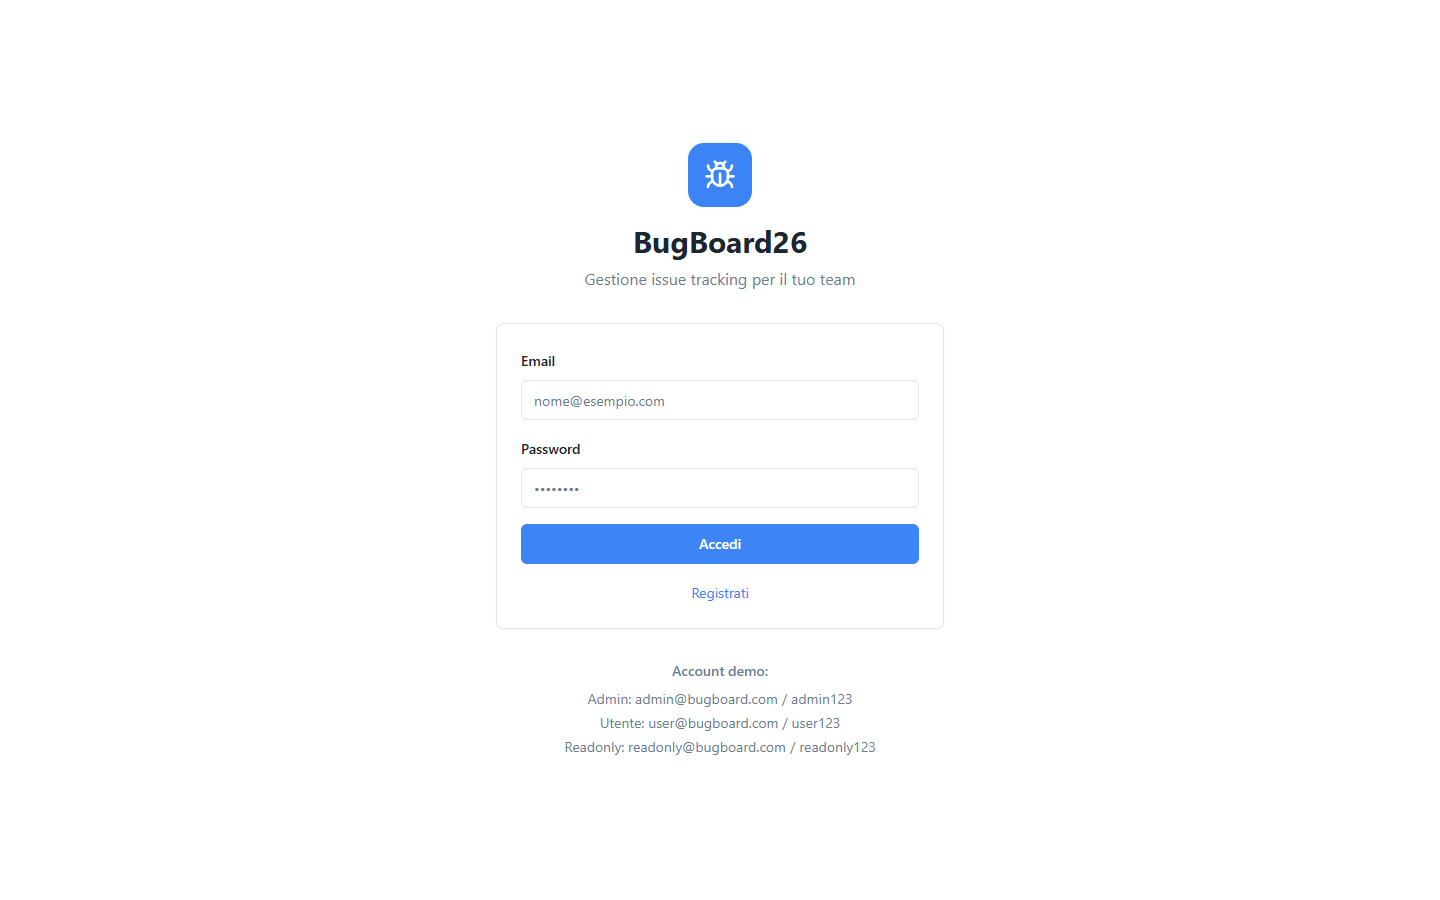
\includegraphics[width=0.85\textwidth]{immagini/mockup_08_notifiche.png}
    \caption{Centro Notifiche: lista degli aggiornamenti sui bug seguiti dall'utente}
    \label{fig:mockup_notifiche}
\end{figure}

\begin{itemize}
    \item \textbf{Scopo}: mostrare all'utente gli aggiornamenti recenti sui bug che lo riguardano (assegnazioni, cambi stato, nuovi commenti)
    \item \textbf{Elementi}: lista notifiche con timestamp, tipo evento e link al bug correlato; indicatore notifiche non lette
\end{itemize}

% ------- 9. PROFILO -------
\subsubsection{Mock-up 9 --- Profilo Utente}

\begin{figure}[H]
    \centering
    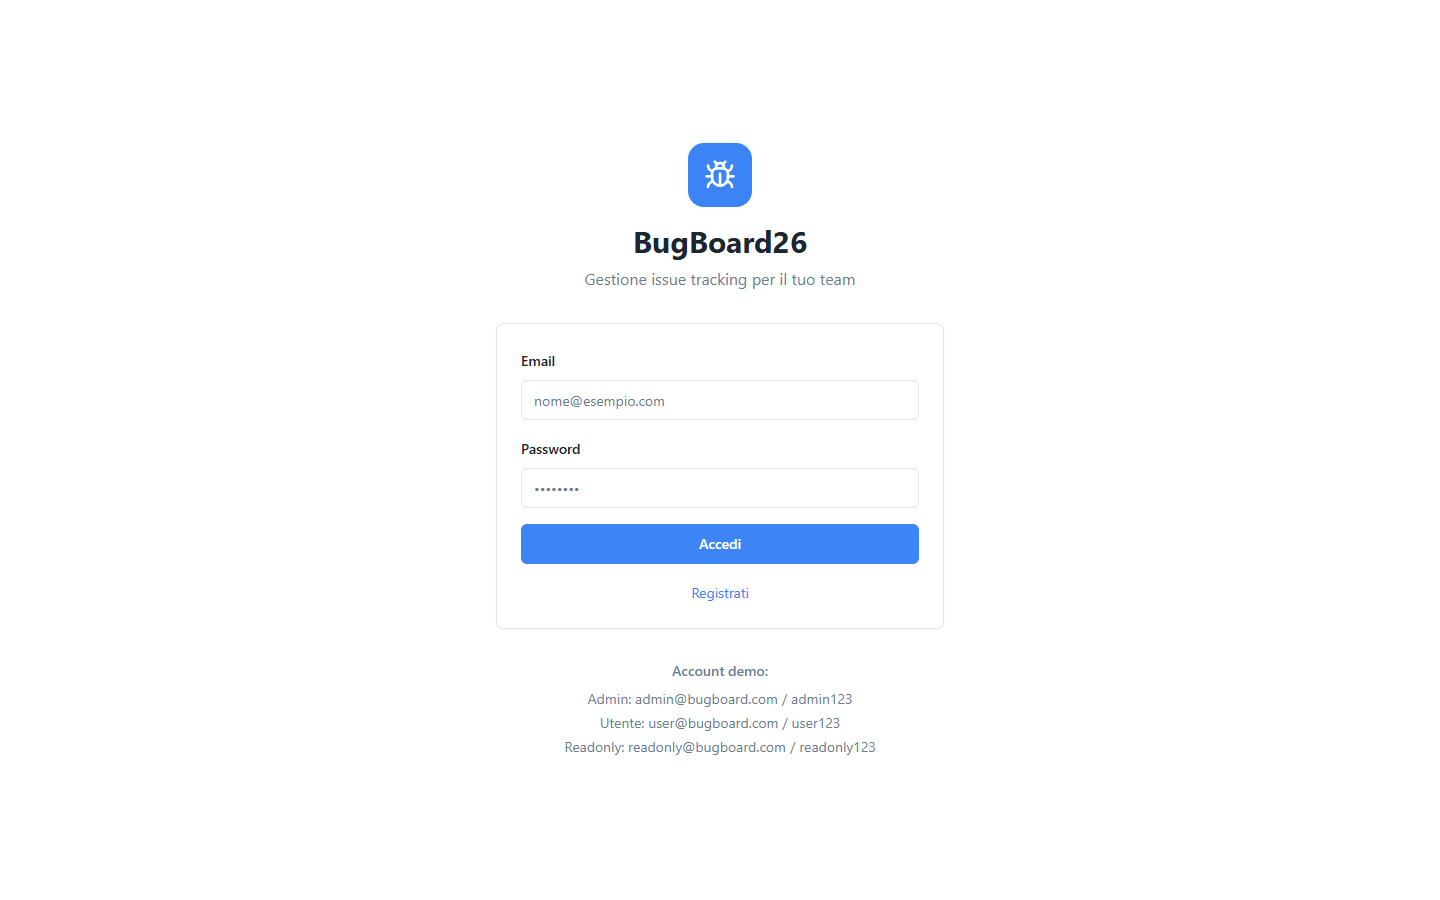
\includegraphics[width=0.85\textwidth]{immagini/mockup_09_profilo.png}
    \caption{Profilo Utente: gestione informazioni personali e cambio password}
    \label{fig:mockup_profilo}
\end{figure}

\begin{itemize}
    \item \textbf{Scopo}: consentire all'utente di visualizzare e modificare le proprie informazioni e la password
    \item \textbf{Elementi}: nome, email, ruolo (in sola lettura), form cambio password con validazione
\end{itemize}

% ------- 10. REPORT MENSILE (UC04) -------
\subsubsection{Mock-up 10 --- Report Mensile \textbf{[UC04]}}

\begin{figure}[H]
    \centering
    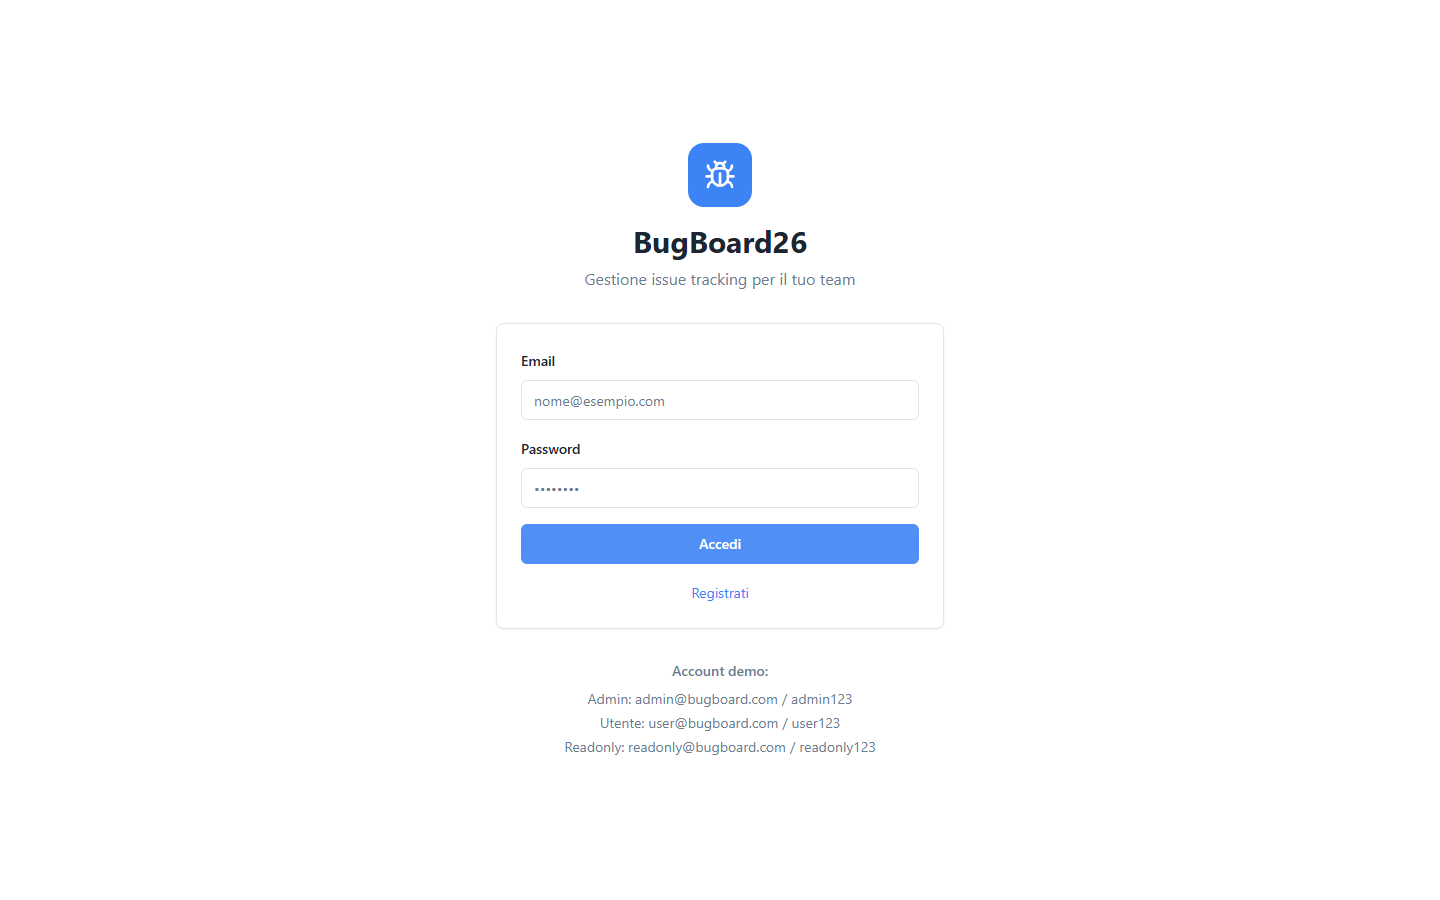
\includegraphics[width=0.85\textwidth]{immagini/mockup_10_report_mensile.png}
    \caption{Report Mensile Admin (UC04): statistiche, grafici e pulsante di export Excel}
    \label{fig:mockup_report}
\end{figure}

\begin{itemize}
    \item \textbf{Caso d'uso}: UC04 --- Generazione report mensile (solo Admin)
    \item \textbf{Elementi}: selettore mese/anno, grafici (distribuzione stato, priorità, trend temporale), tabella riassuntiva metriche, pulsante ``Esporta Excel''
    \item \textbf{Accesso}: solo Admin; gli altri utenti vengono reindirizzati alla Dashboard
\end{itemize}

% ------- 11. GESTIONE UTENTI ADMIN -------
\subsubsection{Mock-up 11 --- Gestione Utenti (Admin)}

\begin{figure}[H]
    \centering
    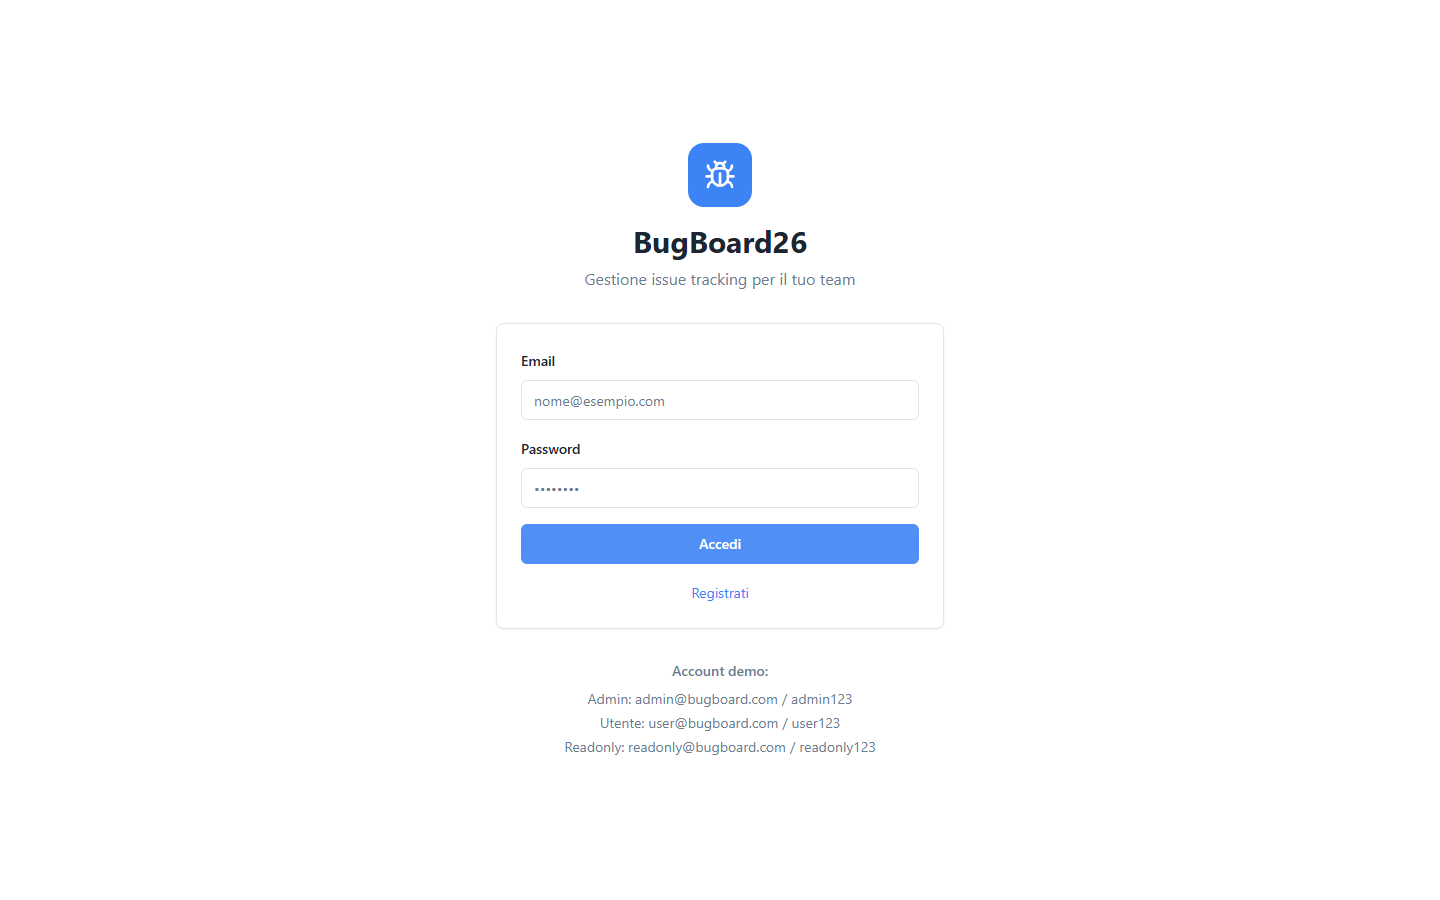
\includegraphics[width=0.85\textwidth]{immagini/mockup_11_admin_utenti.png}
    \caption{Gestione Utenti Admin: lista utenti con ruoli, stato e azioni di modifica}
    \label{fig:mockup_admin_utenti}
\end{figure}

\begin{itemize}
    \item \textbf{Scopo}: permettere all'Admin di gestire gli account del sistema (visualizzazione ruoli, disabilitazione utenti)
    \item \textbf{Elementi}: tabella utenti con email, nome, ruolo e stato; azioni per modifica ruolo e disabilitazione account
\end{itemize}

% ------- 12. ARCHIVIO -------
\subsubsection{Mock-up 12 --- Archivio Bug}

\begin{figure}[H]
    \centering
    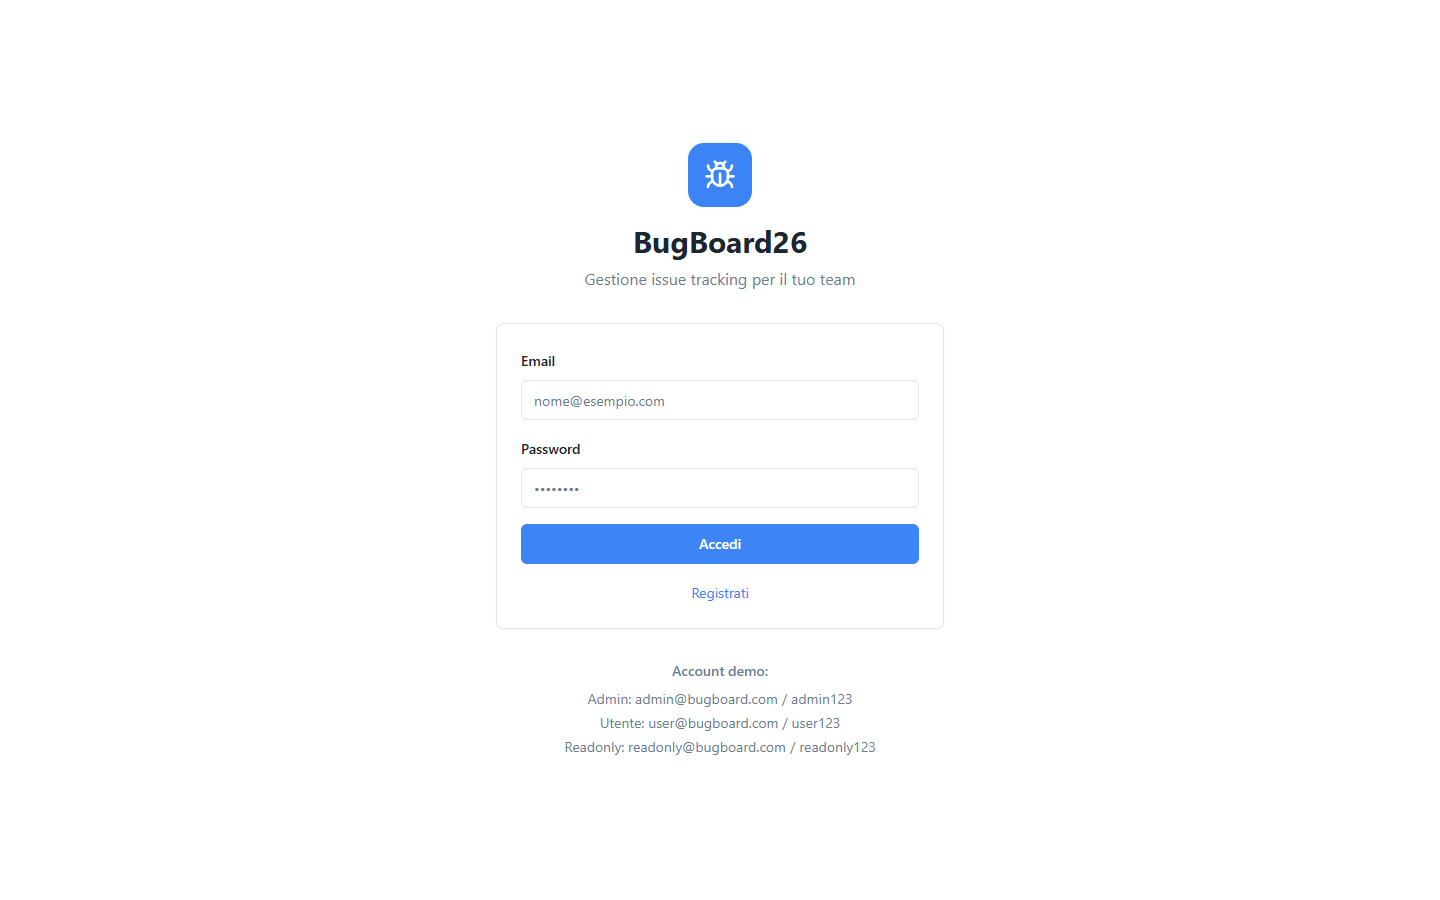
\includegraphics[width=0.85\textwidth]{immagini/mockup_12_archivio.png}
    \caption{Archivio Bug: lista dei bug archiviati con possibilità di consultazione}
    \label{fig:mockup_archivio}
\end{figure}

\begin{itemize}
    \item \textbf{Scopo}: visualizzare i bug archiviati per storico e consultazione senza influire sulla lista attiva
    \item \textbf{Elementi}: tabella bug in stato \textit{Archived} con filtri e ricerca; solo Admin può archiviare/ripristinare bug
\end{itemize}

% ------- 13. EXPORT -------
\subsubsection{Mock-up 13 --- Export Dati}

\begin{figure}[H]
    \centering
    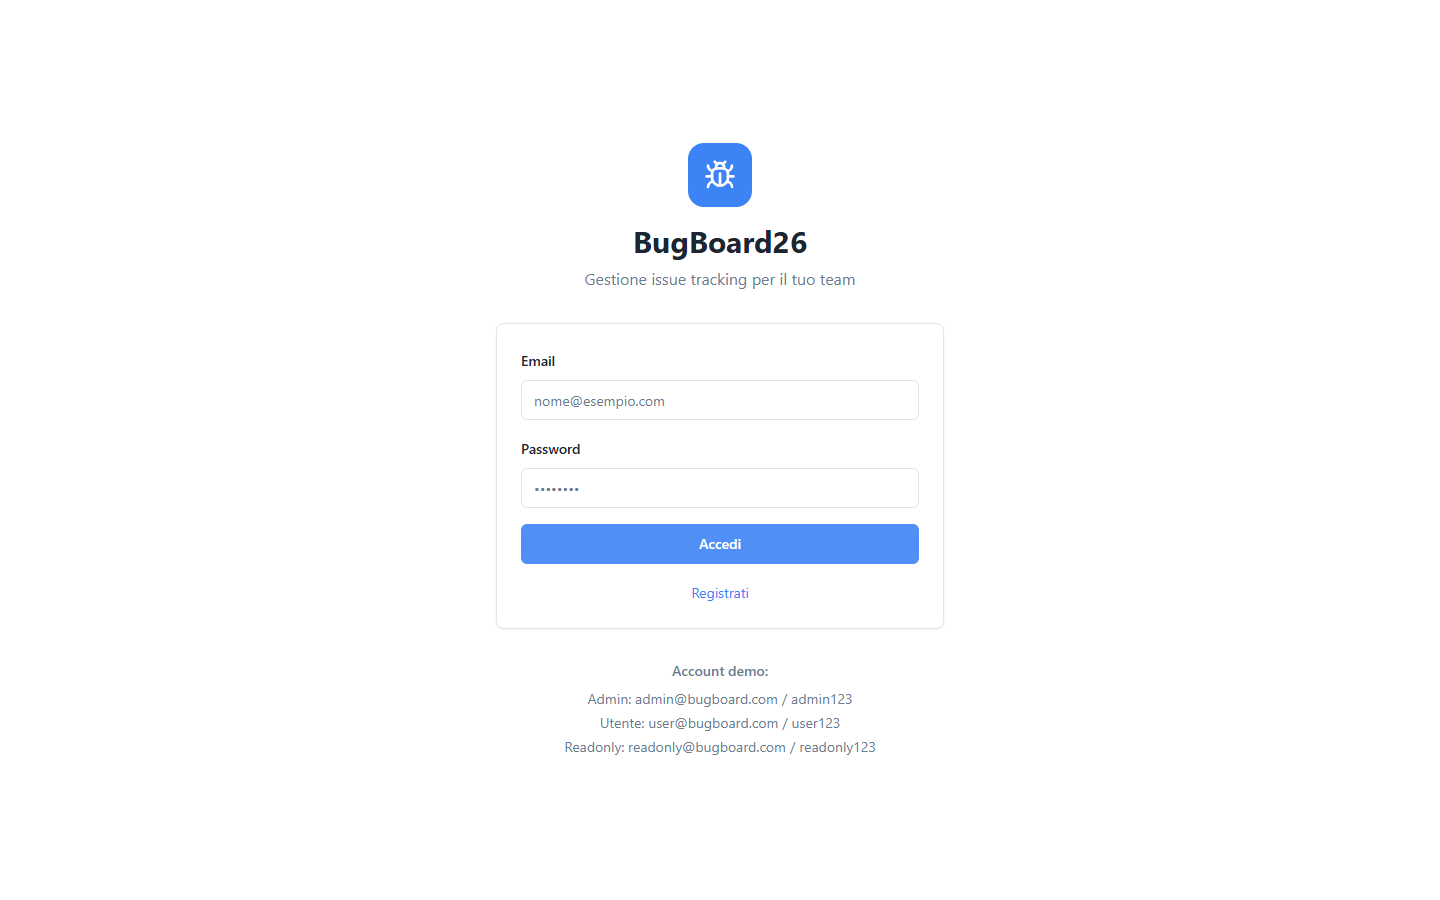
\includegraphics[width=0.85\textwidth]{immagini/mockup_13_export.png}
    \caption{Export Dati: download dell'elenco bug in formato CSV o Excel}
    \label{fig:mockup_export}
\end{figure}

\begin{itemize}
    \item \textbf{Scopo}: consentire l'esportazione dei dati per analisi esterne
    \item \textbf{Elementi}: pulsanti ``Scarica CSV'' e ``Scarica Excel''; i file vengono generati dal backend e scaricati direttamente
\end{itemize}

% ------------------------------------------------------------
\subsection{Osservazioni emerse dalla prototipazione}

La realizzazione del prototipo funzionante ha permesso di identificare alcune scelte migliorative rispetto all'analisi iniziale:

\begin{itemize}
    \item \textbf{Chiarezza dei ruoli}: è stato necessario rendere esplicito nel UI quali azioni sono riservate all'Admin (assegnazione, report, archiviazione, gestione utenti), aggiungendo reindirizzamenti automatici per utenti non autorizzati
    \item \textbf{Filtri immediati}: la lista bug con filtri in tempo reale si è rivelata la funzionalità più usata nelle sessioni di test, confermando la scelta di renderla la pagina principale
    \item \textbf{Badge colorati}: l'uso di badge cromatici per stato, priorità e tipo ha migliorato significativamente la leggibilità della lista bug senza aprire il dettaglio
    \item \textbf{Navigazione mobile}: il menu hamburger con le stesse voci del desktop ha garantito piena parità funzionale su dispositivi mobili
\end{itemize}

% ============================================================

\section{Prototipazione visuale attraverso Mock-up}

La prototipazione visuale di BugBoard26 è stata realizzata direttamente come applicazione React funzionante, con dati simulati (\textit{mock data}). Le schermate qui mostrate sono catture reali del prototipo interattivo, e non semplici bozzetti grafici. Questo approccio ha permesso di validare il flusso utente in modo concreto fin dalla fase di analisi.

% ------------------------------------------------------------
\subsection{Scelte Progettuali}

\subsubsection{Layout e Navigazione}
\begin{itemize}
    \item \textbf{Header fisso}: barra superiore con logo, link alle sezioni principali (Dashboard, Bug, Report, Admin) e menu utente con avatar, email e pulsante logout
    \item \textbf{Navigazione mobile}: menu a comparsa (hamburger) con le stesse voci, ottimizzato per touch
    \item \textbf{Layout responsive}: design \textit{mobile-first} realizzato con Tailwind CSS; le griglie si adattano automaticamente a qualsiasi larghezza schermo
\end{itemize}

\subsubsection{Palette Colori e Badge}
\begin{itemize}
    \item \textbf{Priorità}: \textit{Critical} (rosso), \textit{High} (arancione), \textit{Medium} (giallo), \textit{Low} (verde)
    \item \textbf{Stato}: \textit{Todo} (grigio chiaro), \textit{In Progress} (blu), \textit{Resolved} (verde), \textit{Archived} (grigio scuro)
    \item \textbf{Tipo}: \textit{Bug} (rosso), \textit{Feature} (viola), \textit{Enhancement} (azzurro)
    \item \textbf{Azioni primarie}: blu (\texttt{\#007BFF}); superfici neutre: grigi Tailwind
\end{itemize}

\subsubsection{Componenti UI riutilizzati}
Tutti i componenti sono basati su \textbf{Radix UI} e \textbf{shadcn/ui}: Button, Card, Select, Dialog, Badge, Table, Toast, DropdownMenu. Questo garantisce coerenza visiva e accessibilità WCAG 2.1 out-of-the-box.

% ------------------------------------------------------------
\subsection{Mock-up delle interfacce utente}

Di seguito sono illustrate le schermate principali del prototipo, raggruppate per funzionalità. Le schermate contrassegnate con \textbf{[UC0X]} corrispondono direttamente ai casi d'uso formalizzati nella sezione precedente.

% ------- 1. LOGIN -------
\subsubsection{Mock-up 1 --- Pagina di Login}

\begin{figure}[H]
    \centering
    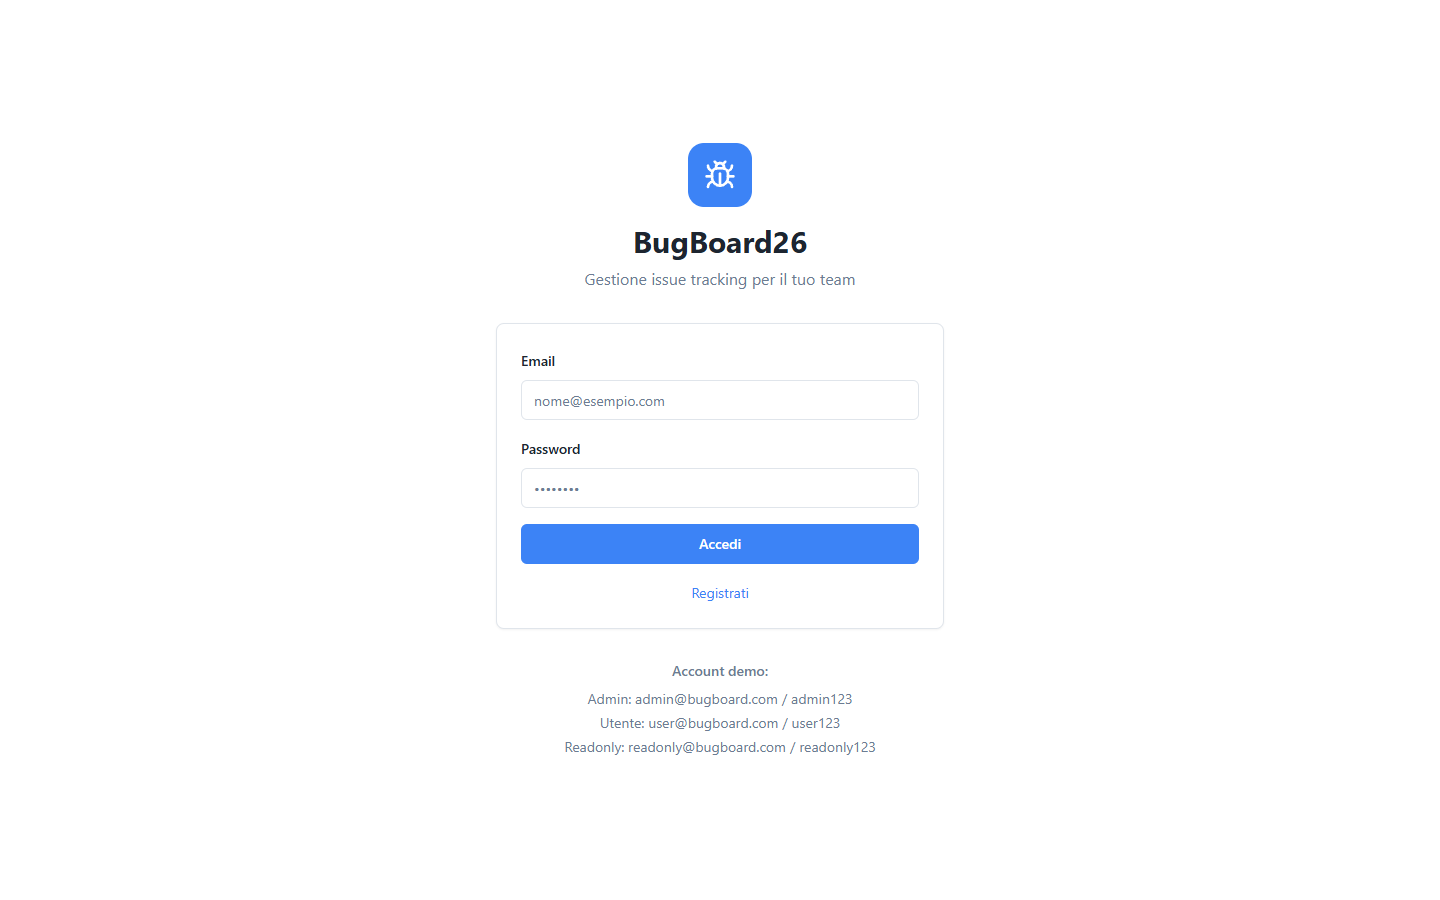
\includegraphics[width=0.85\textwidth]{immagini/mockup_01_login.png}
    \caption{Pagina di Login: form con email e password, pulsante di accesso}
    \label{fig:mockup_login}
\end{figure}

\begin{itemize}
    \item \textbf{Scopo}: autenticazione dell'utente al sistema
    \item \textbf{Elementi}: campo email, campo password, pulsante ``Accedi'', link alla pagina di registrazione
    \item \textbf{Comportamento}: in caso di credenziali errate viene mostrato un messaggio di errore inline; in caso di successo l'utente viene reindirizzato alla Dashboard
\end{itemize}

% ------- 2. REGISTRAZIONE -------
\subsubsection{Mock-up 2 --- Pagina di Registrazione}

\begin{figure}[H]
    \centering
    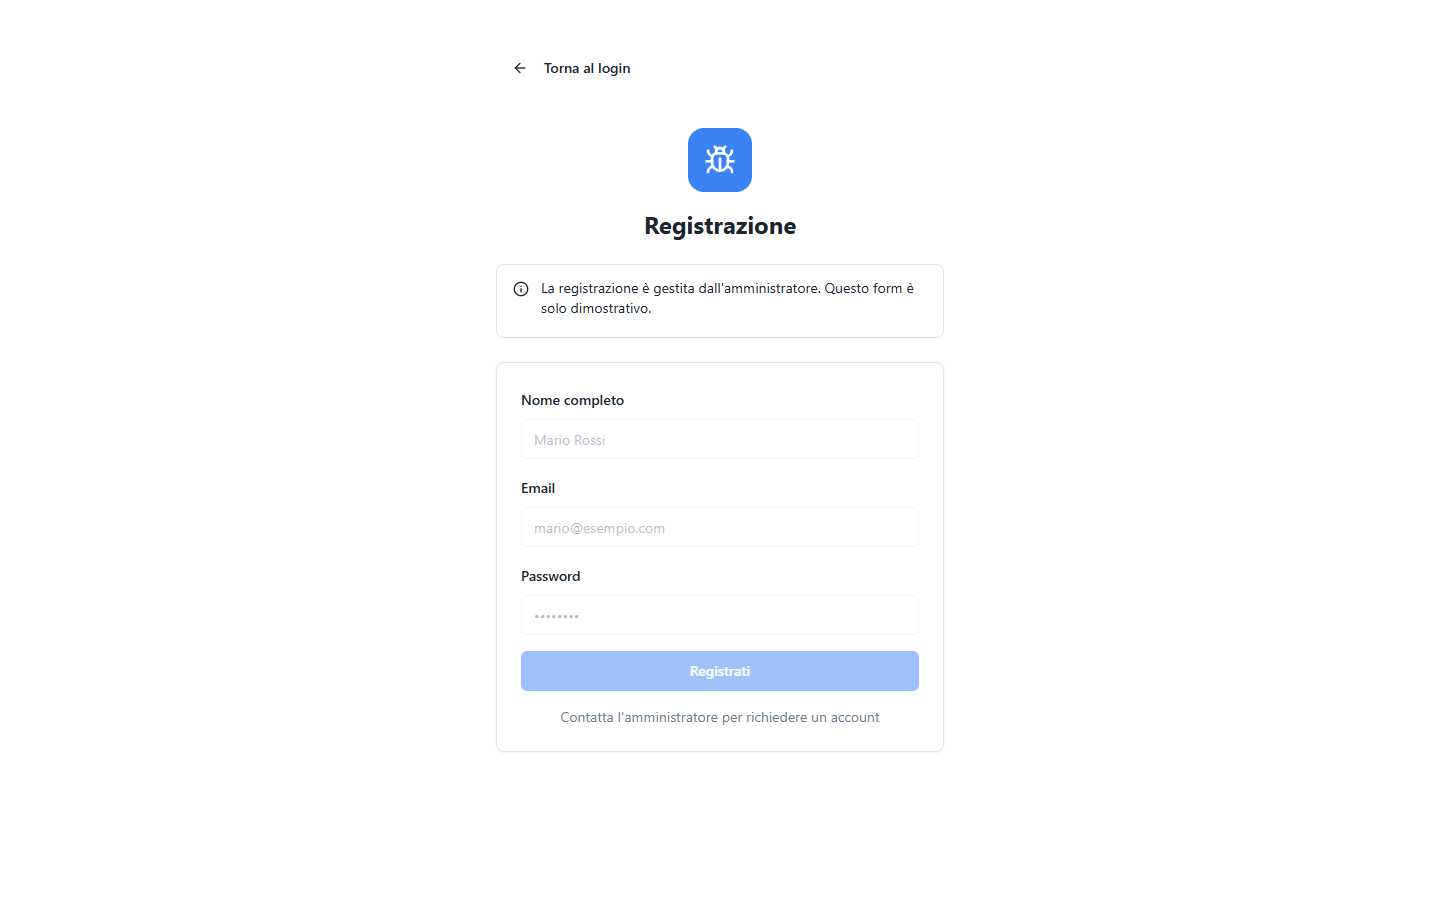
\includegraphics[width=0.85\textwidth]{immagini/mockup_02_register.png}
    \caption{Pagina di Registrazione: form con dati personali e creazione account}
    \label{fig:mockup_register}
\end{figure}

\begin{itemize}
    \item \textbf{Scopo}: creazione di un nuovo account utente
    \item \textbf{Elementi}: campi nome, email, password, conferma password; pulsante ``Registrati''
    \item \textbf{Validazione}: i campi vengono validati in tempo reale con messaggi di errore inline
\end{itemize}

% ------- 3. HOME -------
\subsubsection{Mock-up 3 --- Home / Dashboard}

\begin{figure}[H]
    \centering
    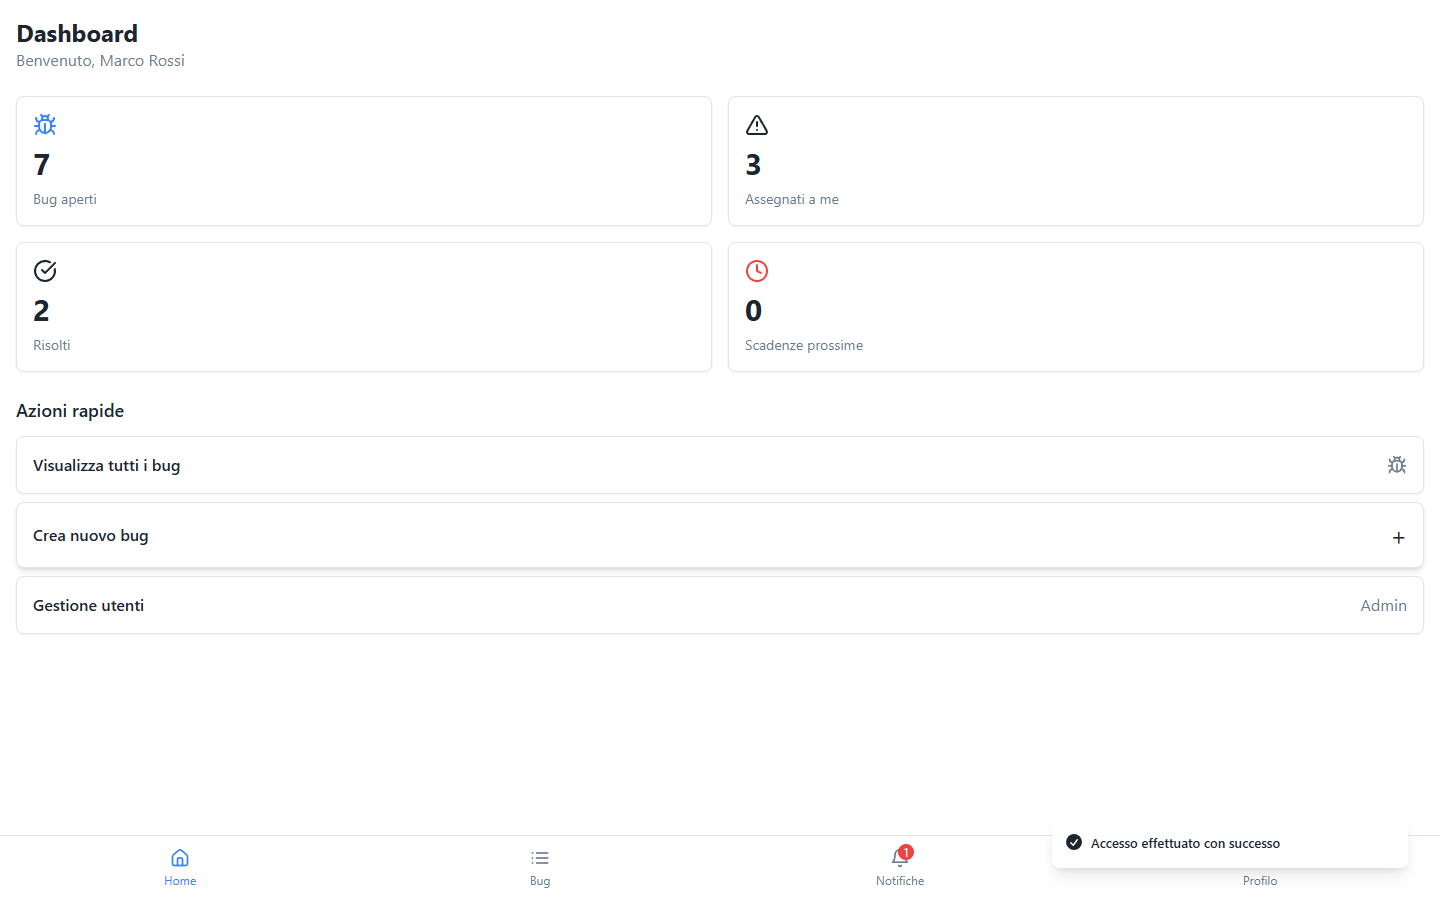
\includegraphics[width=0.85\textwidth]{immagini/mockup_03_home_dashboard.png}
    \caption{Home Dashboard: panoramica delle metriche principali e accessi rapidi}
    \label{fig:mockup_home}
\end{figure}

\begin{itemize}
    \item \textbf{Scopo}: fornire una panoramica immediata dello stato del sistema dopo il login
    \item \textbf{Elementi}: card metriche (bug aperti, assegnati a me, risolti, scadenze prossime), header con navigazione principale
    \item \textbf{Accessi rapidi}: da qui si può navigare alla lista bug, al form di creazione e ai report
\end{itemize}

% ------- 4. LISTA BUG -------
\subsubsection{Mock-up 4 --- Lista Bug con Filtri}

\begin{figure}[H]
    \centering
    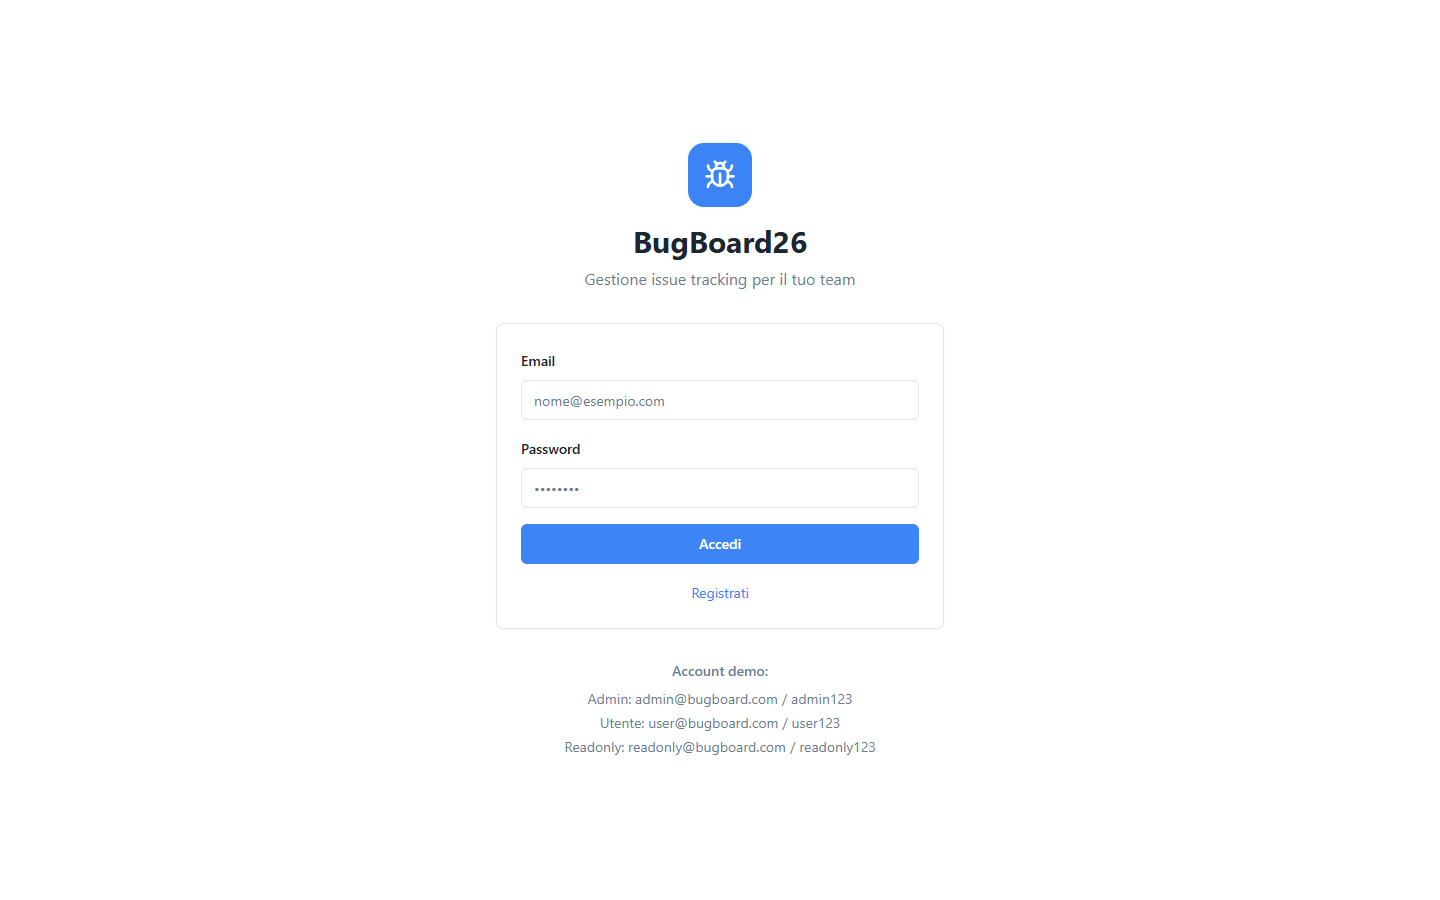
\includegraphics[width=0.85\textwidth]{immagini/mockup_04_lista_bug.png}
    \caption{Lista Bug: tabella con filtri per tipo, stato, priorità e ricerca testuale}
    \label{fig:mockup_lista_bug}
\end{figure}

\begin{itemize}
    \item \textbf{Scopo}: visualizzazione e filtraggio dell'elenco completo dei bug
    \item \textbf{Elementi}: barra filtri orizzontale (tipo, stato, priorità), campo ricerca full-text, tabella bug con badge colorati, paginazione
    \item \textbf{Interazione}: clic su una riga apre il dettaglio del bug; i filtri si applicano in tempo reale
\end{itemize}

% ------- 5. DETTAGLIO BUG -------
\subsubsection{Mock-up 5 --- Dettaglio Bug}

\begin{figure}[H]
    \centering
    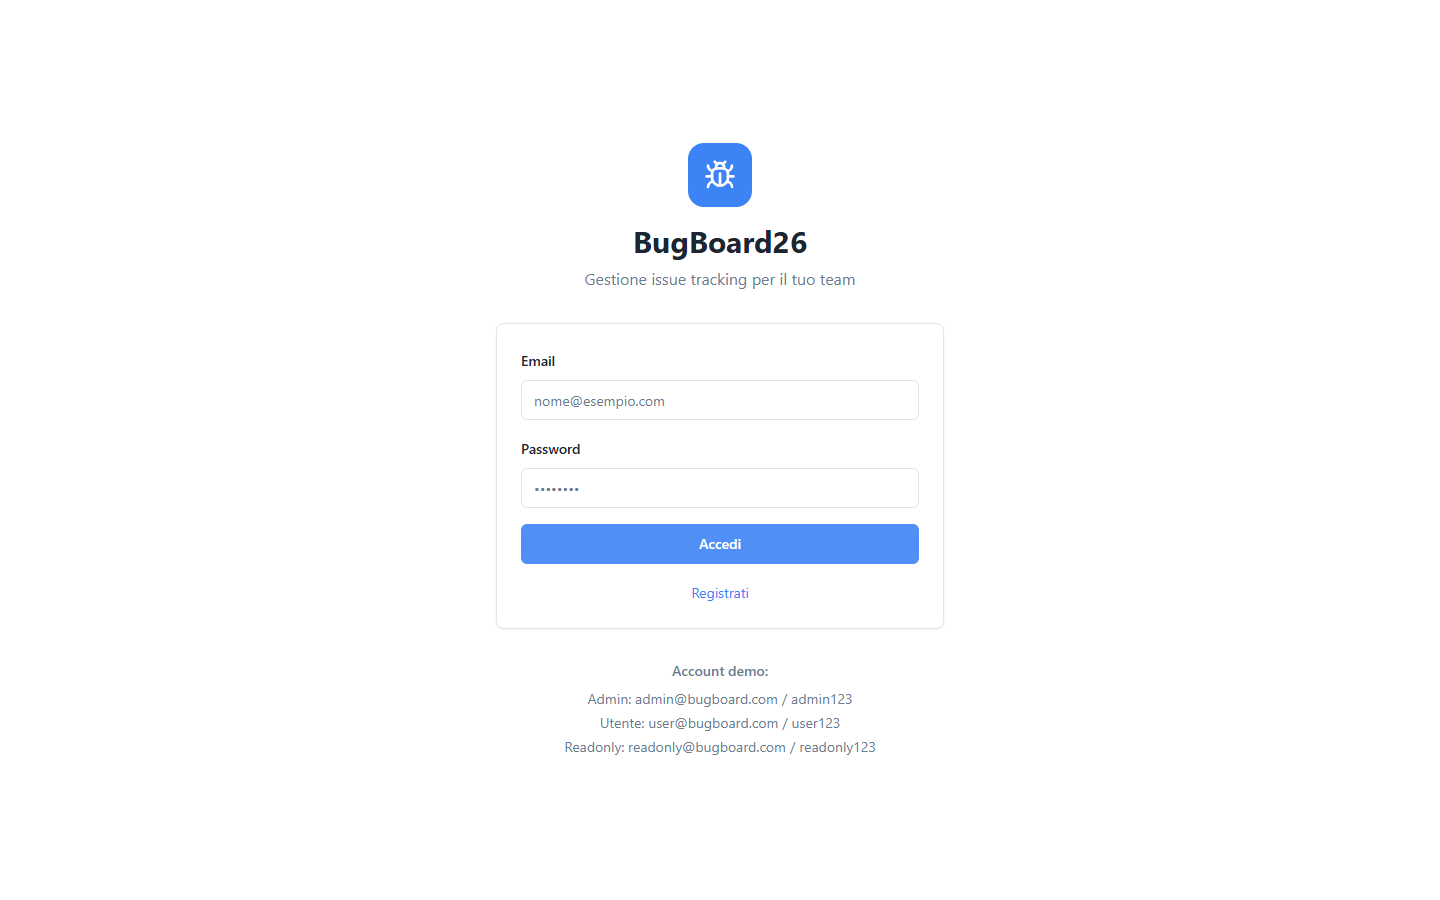
\includegraphics[width=0.85\textwidth]{immagini/mockup_05_dettaglio_bug.png}
    \caption{Dettaglio Bug: informazioni complete, commenti, storico modifiche e azioni disponibili}
    \label{fig:mockup_dettaglio_bug}
\end{figure}

\begin{itemize}
    \item \textbf{Scopo}: visualizzazione completa di un bug specifico e gestione delle azioni disponibili
    \item \textbf{Elementi}: header con titolo, stato e priorità; sezioni descrizione, commenti, allegati, storico; barra azioni laterale (modifica, assegna, risolvi, archivia, duplica)
    \item \textbf{Azioni visibili}: dipendono dal ruolo dell'utente (USER vede meno azioni rispetto ad Admin)
\end{itemize}

% ------- 6. FORM CREAZIONE BUG (UC01) -------
\subsubsection{Mock-up 6 --- Form Creazione/Modifica Bug \textbf{[UC01]}}

\begin{figure}[H]
    \centering
    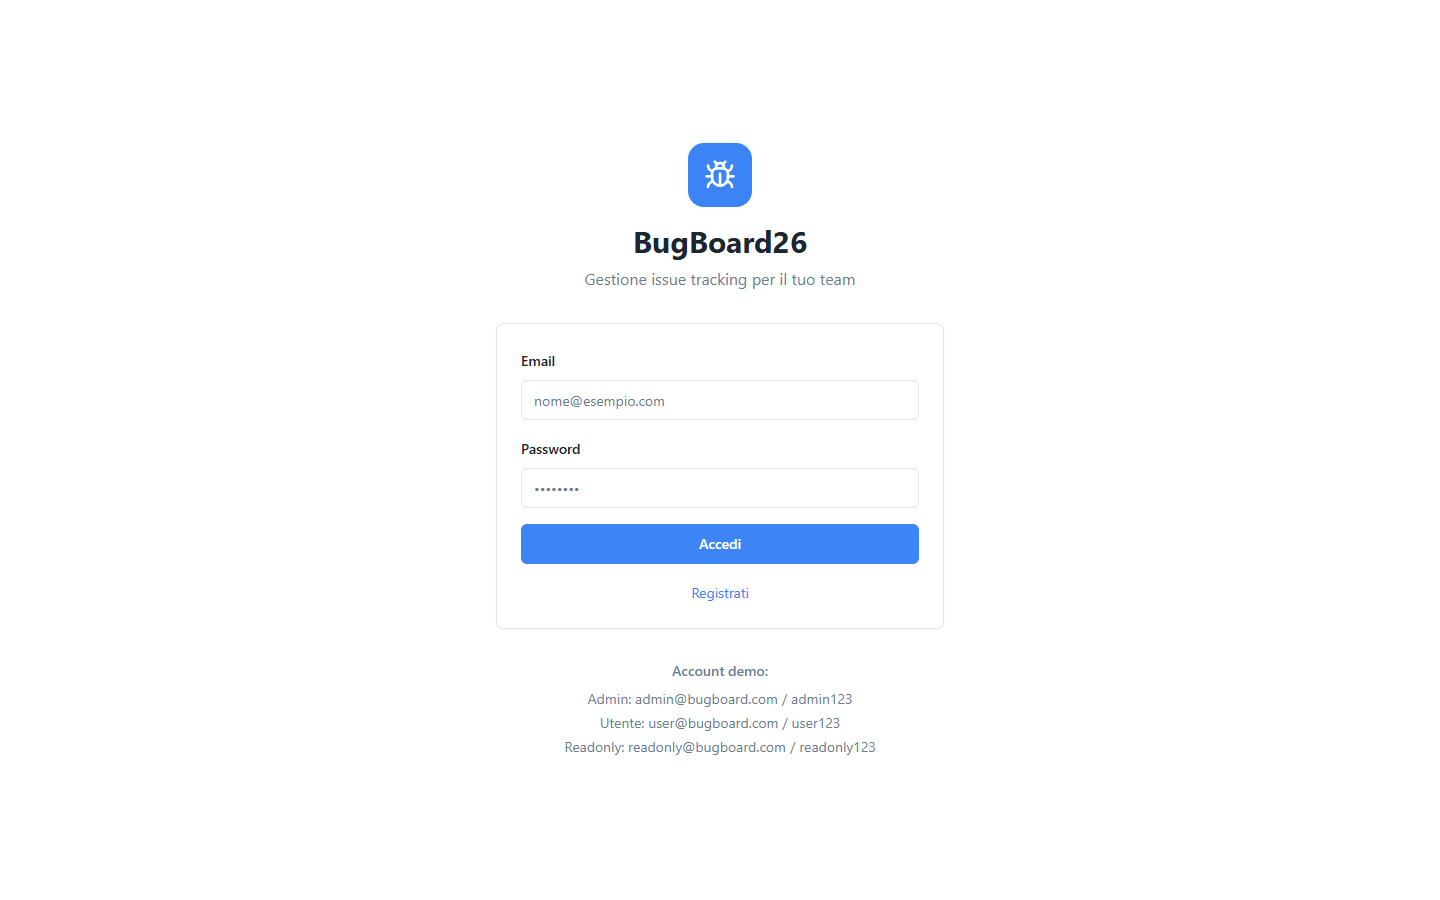
\includegraphics[width=0.85\textwidth]{immagini/mockup_06_form_creazione_bug.png}
    \caption{Form Creazione Bug (UC01): campi titolo, tipo, priorità, descrizione, label, allegati}
    \label{fig:mockup_form_bug}
\end{figure}

\begin{itemize}
    \item \textbf{Caso d'uso}: UC01 --- Creazione nuovo bug
    \item \textbf{Elementi}: campo titolo, selettori tipo e priorità, area di testo descrizione, selezione label multipla, upload allegati immagine, selezione assegnatario opzionale, pulsante ``Salva''
    \item \textbf{Validazione}: i campi obbligatori (titolo, tipo, priorità) sono evidenziati se lasciati vuoti; il formato e la dimensione degli allegati sono verificati prima dell'invio
\end{itemize}

% ------- 7. ASSEGNAZIONE BUG (UC02) -------
\subsubsection{Mock-up 7 --- Assegnazione Bug \textbf{[UC02]}}

\begin{figure}[H]
    \centering
    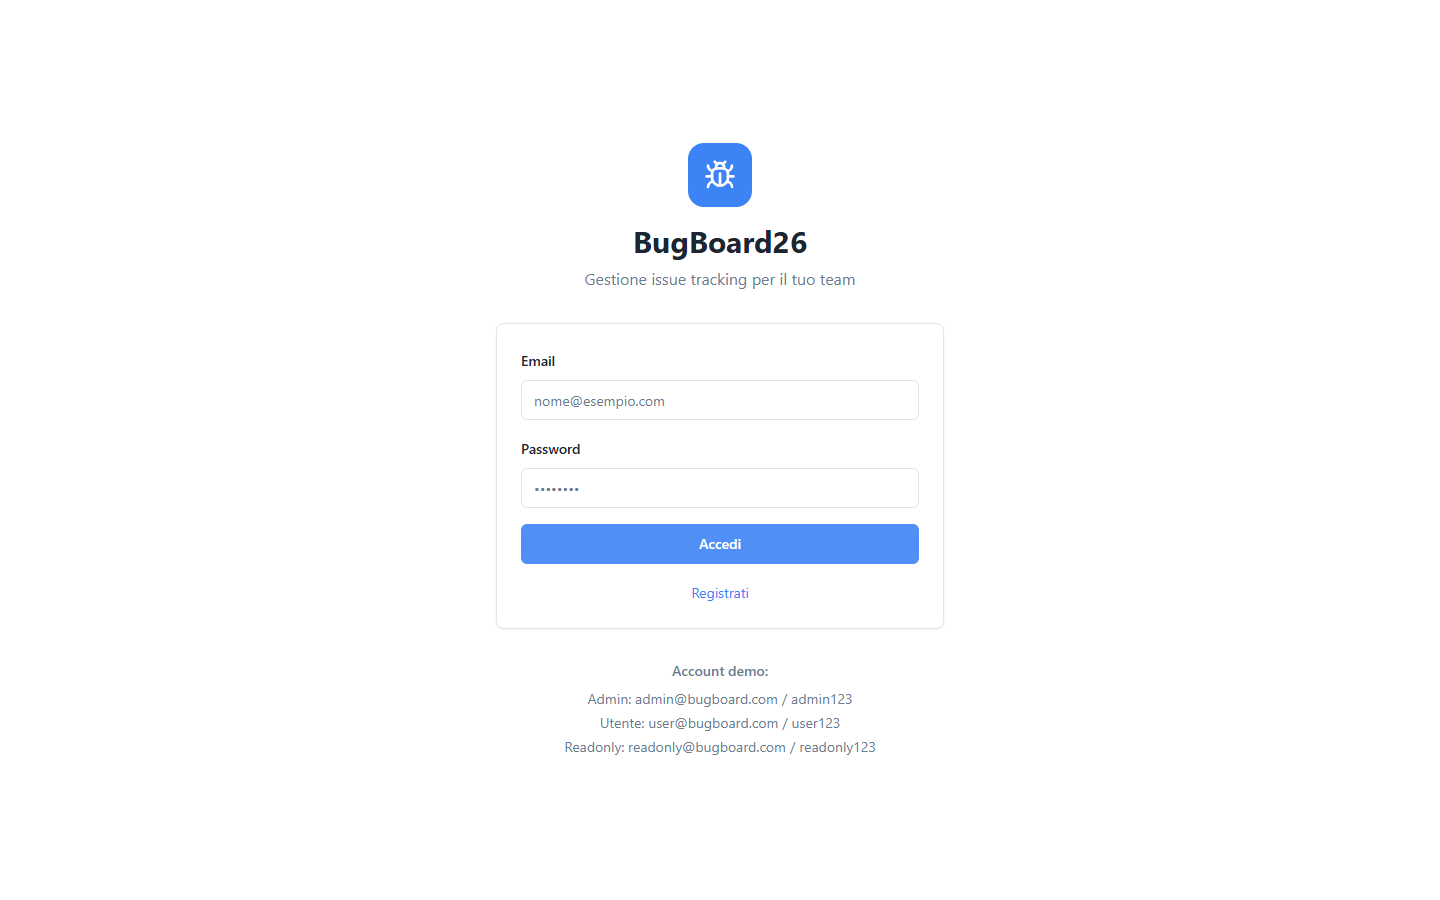
\includegraphics[width=0.85\textwidth]{immagini/mockup_07_assegnazione_bug.png}
    \caption{Assegnazione Bug (UC02): selezione dell'utente a cui assegnare il bug}
    \label{fig:mockup_assegnazione}
\end{figure}

\begin{itemize}
    \item \textbf{Caso d'uso}: UC02 --- Assegnazione bug a un utente (solo Admin)
    \item \textbf{Elementi}: select per la scelta dell'utente assegnatario, pulsante conferma
    \item \textbf{Accesso}: questa schermata è accessibile solo agli utenti con ruolo Admin; un USER viene reindirizzato alla Dashboard
\end{itemize}

% ------- 8. NOTIFICHE -------
\subsubsection{Mock-up 8 --- Notifiche}

\begin{figure}[H]
    \centering
    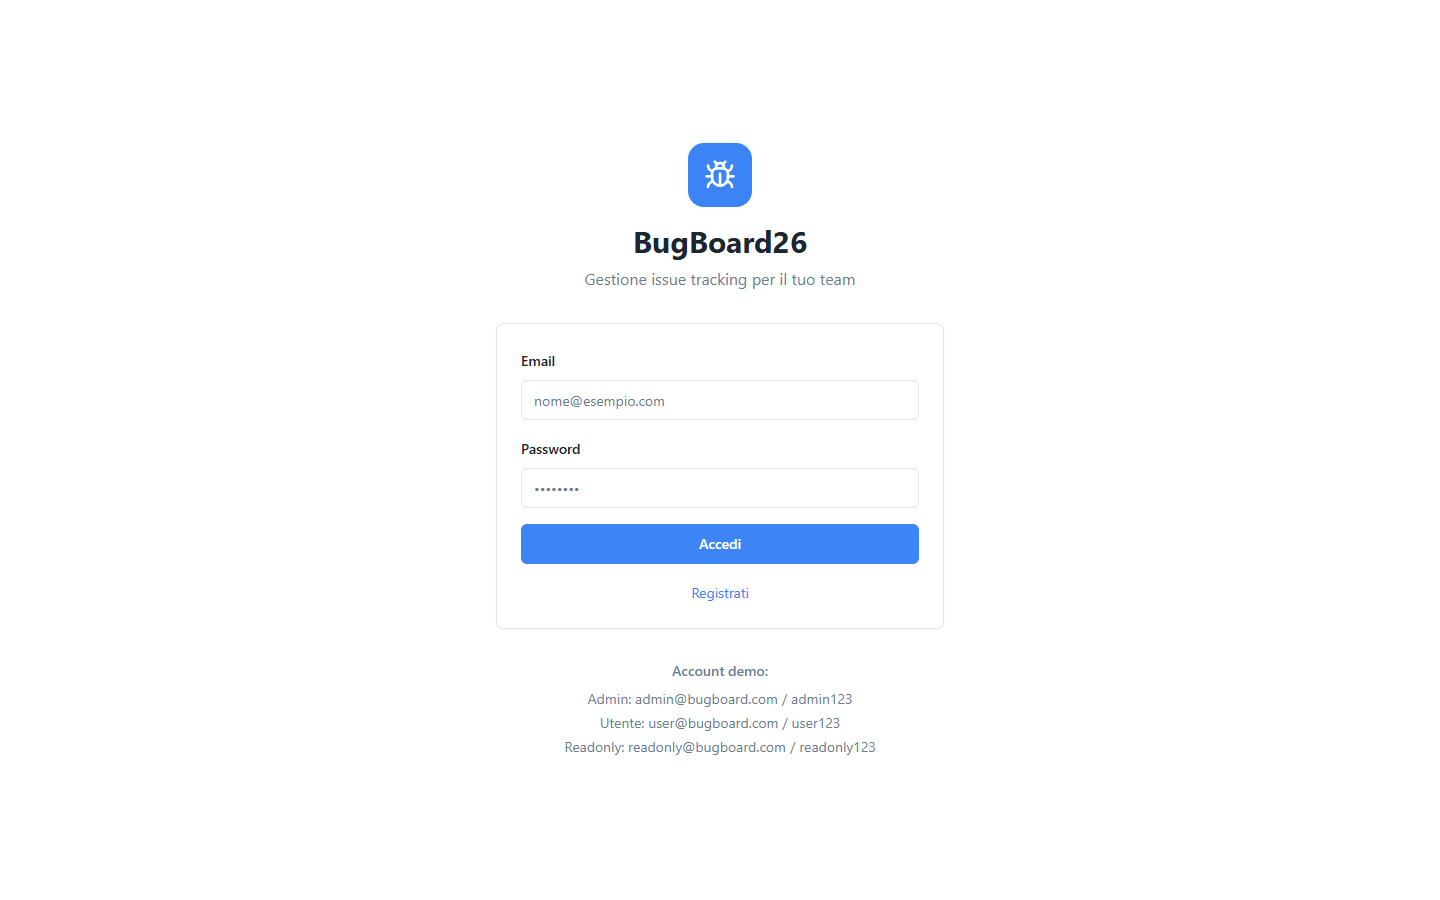
\includegraphics[width=0.85\textwidth]{immagini/mockup_08_notifiche.png}
    \caption{Centro Notifiche: lista degli aggiornamenti sui bug seguiti dall'utente}
    \label{fig:mockup_notifiche}
\end{figure}

\begin{itemize}
    \item \textbf{Scopo}: mostrare all'utente gli aggiornamenti recenti sui bug che lo riguardano (assegnazioni, cambi stato, nuovi commenti)
    \item \textbf{Elementi}: lista notifiche con timestamp, tipo evento e link al bug correlato; indicatore notifiche non lette
\end{itemize}

% ------- 9. PROFILO -------
\subsubsection{Mock-up 9 --- Profilo Utente}

\begin{figure}[H]
    \centering
    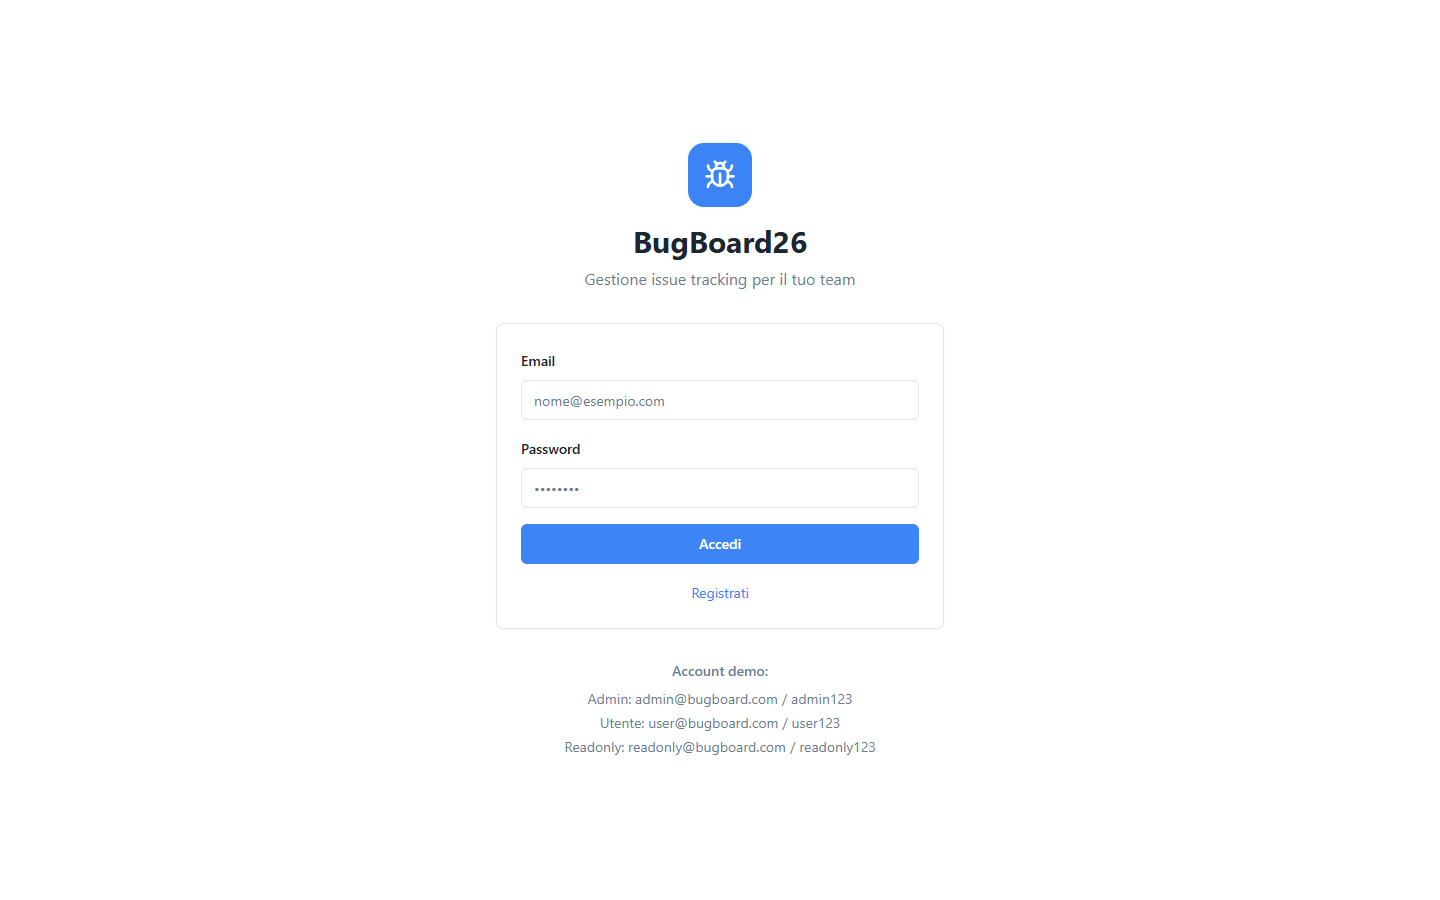
\includegraphics[width=0.85\textwidth]{immagini/mockup_09_profilo.png}
    \caption{Profilo Utente: gestione informazioni personali e cambio password}
    \label{fig:mockup_profilo}
\end{figure}

\begin{itemize}
    \item \textbf{Scopo}: consentire all'utente di visualizzare e modificare le proprie informazioni e la password
    \item \textbf{Elementi}: nome, email, ruolo (in sola lettura), form cambio password con validazione
\end{itemize}

% ------- 10. REPORT MENSILE (UC04) -------
\subsubsection{Mock-up 10 --- Report Mensile \textbf{[UC04]}}

\begin{figure}[H]
    \centering
    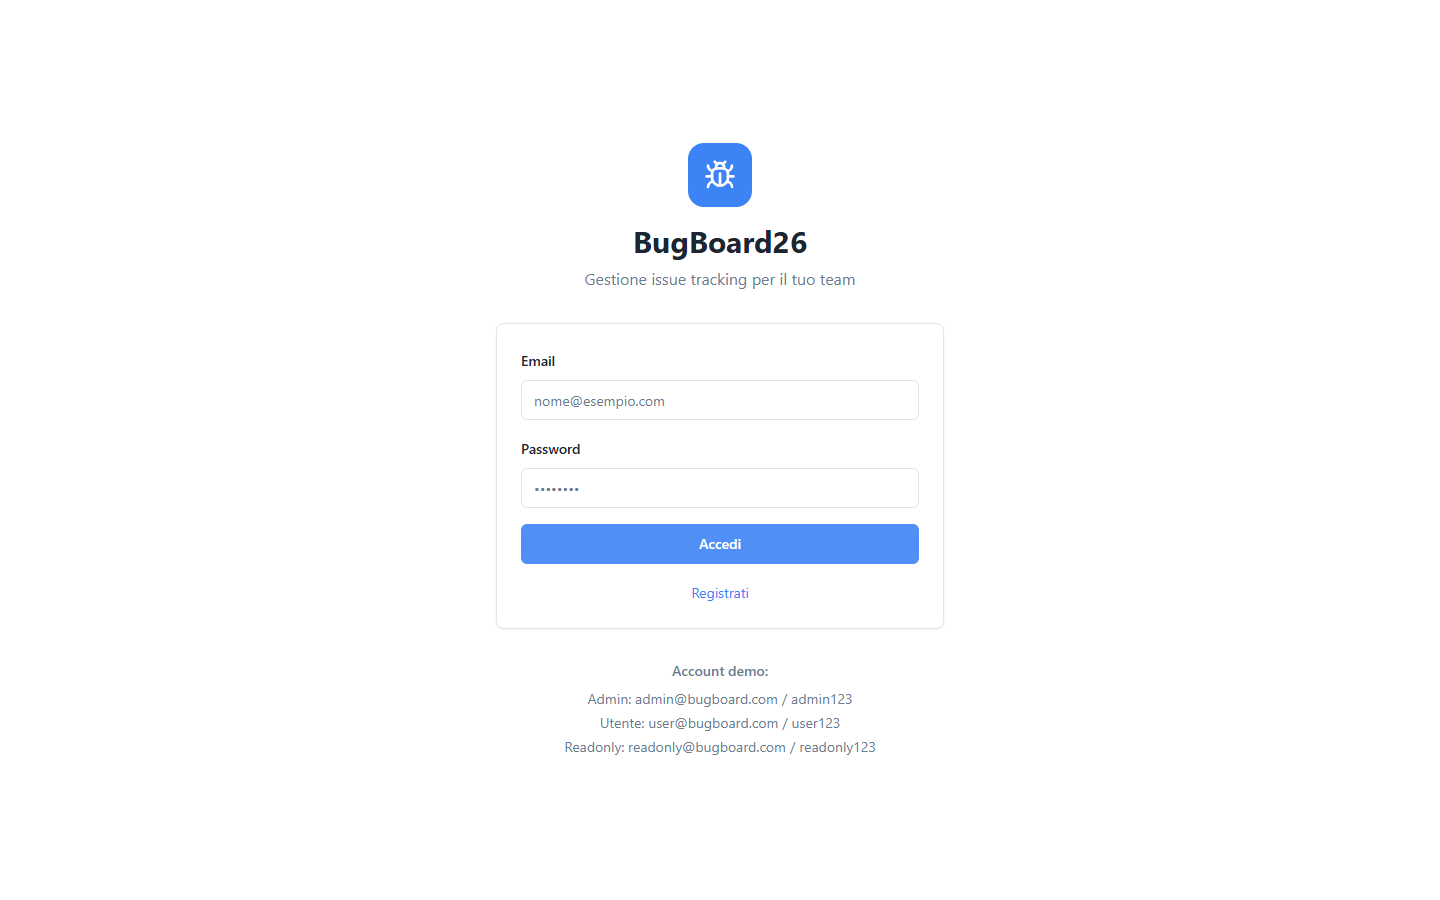
\includegraphics[width=0.85\textwidth]{immagini/mockup_10_report_mensile.png}
    \caption{Report Mensile Admin (UC04): statistiche, grafici e pulsante di export Excel}
    \label{fig:mockup_report}
\end{figure}

\begin{itemize}
    \item \textbf{Caso d'uso}: UC04 --- Generazione report mensile (solo Admin)
    \item \textbf{Elementi}: selettore mese/anno, grafici (distribuzione stato, priorità, trend temporale), tabella riassuntiva metriche, pulsante ``Esporta Excel''
    \item \textbf{Accesso}: solo Admin; gli altri utenti vengono reindirizzati alla Dashboard
\end{itemize}

% ------- 11. GESTIONE UTENTI ADMIN -------
\subsubsection{Mock-up 11 --- Gestione Utenti (Admin)}

\begin{figure}[H]
    \centering
    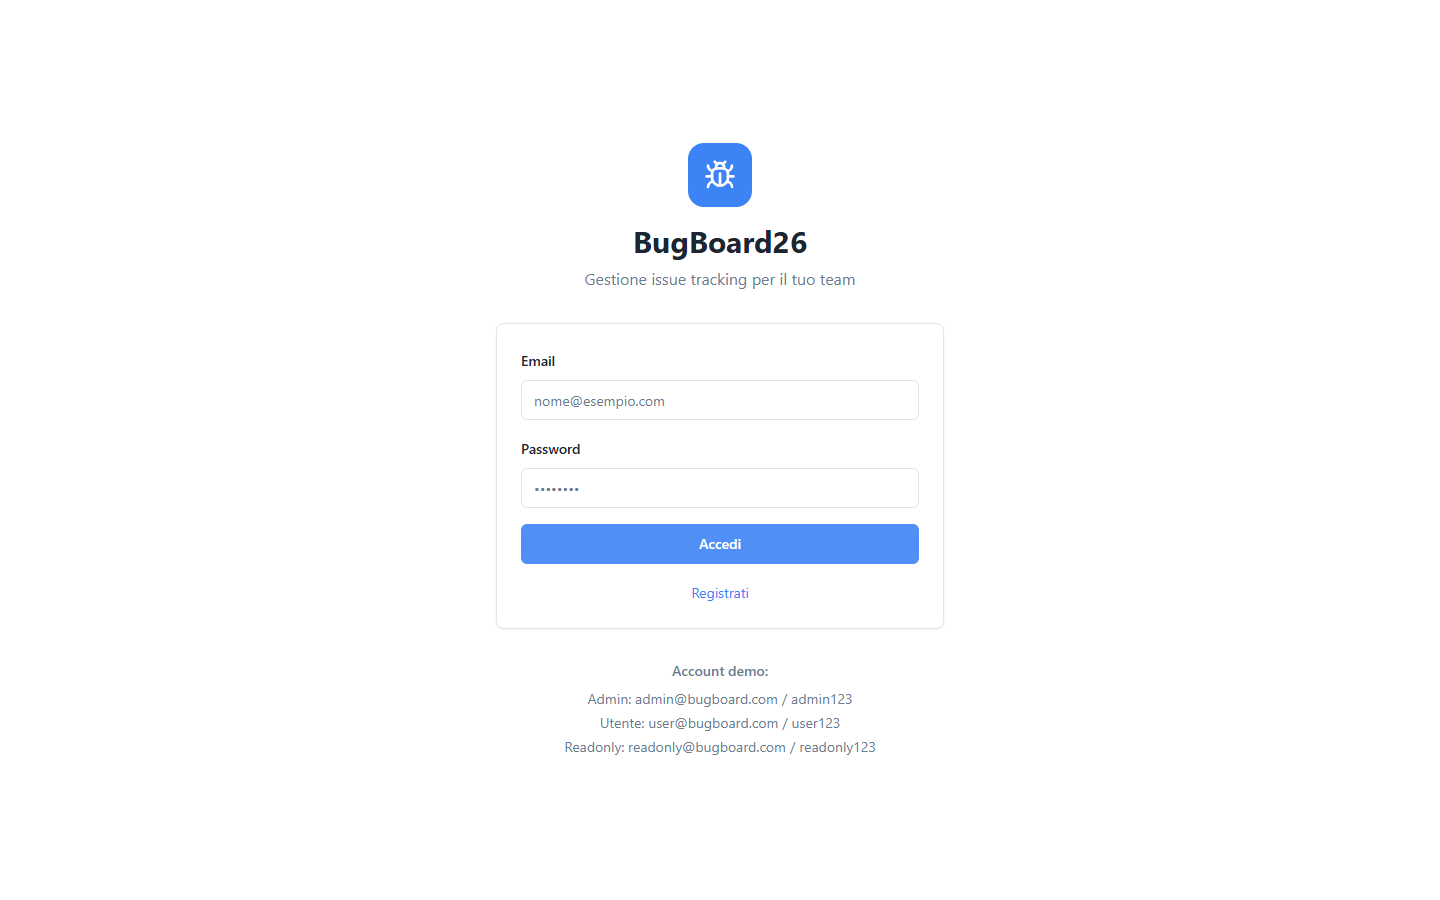
\includegraphics[width=0.85\textwidth]{immagini/mockup_11_admin_utenti.png}
    \caption{Gestione Utenti Admin: lista utenti con ruoli, stato e azioni di modifica}
    \label{fig:mockup_admin_utenti}
\end{figure}

\begin{itemize}
    \item \textbf{Scopo}: permettere all'Admin di gestire gli account del sistema (visualizzazione ruoli, disabilitazione utenti)
    \item \textbf{Elementi}: tabella utenti con email, nome, ruolo e stato; azioni per modifica ruolo e disabilitazione account
\end{itemize}

% ------- 12. ARCHIVIO -------
\subsubsection{Mock-up 12 --- Archivio Bug}

\begin{figure}[H]
    \centering
    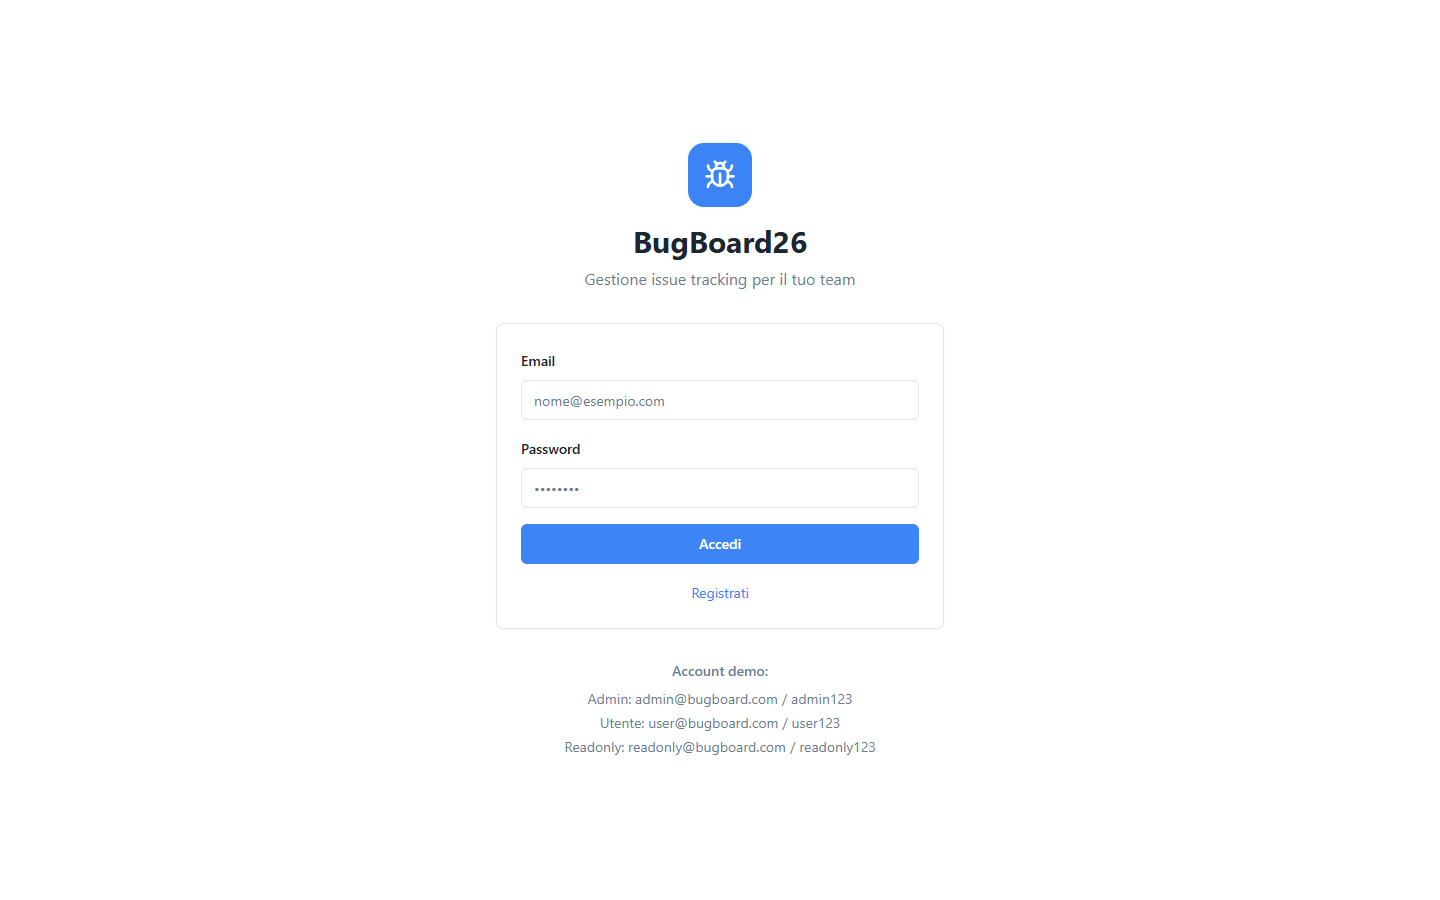
\includegraphics[width=0.85\textwidth]{immagini/mockup_12_archivio.png}
    \caption{Archivio Bug: lista dei bug archiviati con possibilità di consultazione}
    \label{fig:mockup_archivio}
\end{figure}

\begin{itemize}
    \item \textbf{Scopo}: visualizzare i bug archiviati per storico e consultazione senza influire sulla lista attiva
    \item \textbf{Elementi}: tabella bug in stato \textit{Archived} con filtri e ricerca; solo Admin può archiviare/ripristinare bug
\end{itemize}

% ------- 13. EXPORT -------
\subsubsection{Mock-up 13 --- Export Dati}

\begin{figure}[H]
    \centering
    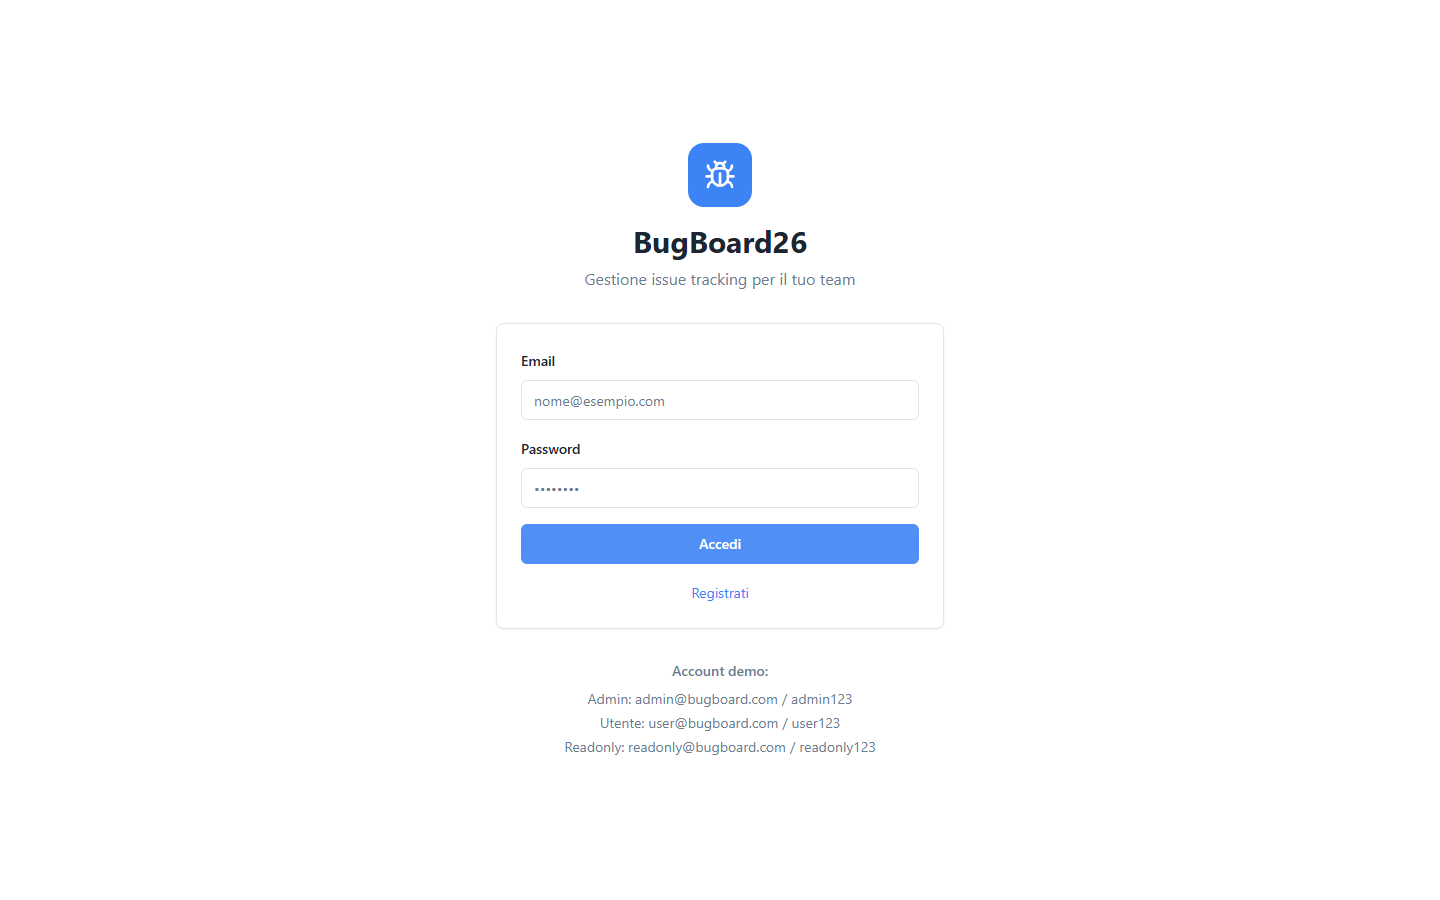
\includegraphics[width=0.85\textwidth]{immagini/mockup_13_export.png}
    \caption{Export Dati: download dell'elenco bug in formato CSV o Excel}
    \label{fig:mockup_export}
\end{figure}

\begin{itemize}
    \item \textbf{Scopo}: consentire l'esportazione dei dati per analisi esterne
    \item \textbf{Elementi}: pulsanti ``Scarica CSV'' e ``Scarica Excel''; i file vengono generati dal backend e scaricati direttamente
\end{itemize}

% ------------------------------------------------------------
\subsection{Osservazioni emerse dalla prototipazione}

La realizzazione del prototipo funzionante ha permesso di identificare alcune scelte migliorative rispetto all'analisi iniziale:

\begin{itemize}
    \item \textbf{Chiarezza dei ruoli}: è stato necessario rendere esplicito nel UI quali azioni sono riservate all'Admin (assegnazione, report, archiviazione, gestione utenti), aggiungendo reindirizzamenti automatici per utenti non autorizzati
    \item \textbf{Filtri immediati}: la lista bug con filtri in tempo reale si è rivelata la funzionalità più usata nelle sessioni di test, confermando la scelta di renderla la pagina principale
    \item \textbf{Badge colorati}: l'uso di badge cromatici per stato, priorità e tipo ha migliorato significativamente la leggibilità della lista bug senza aprire il dettaglio
    \item \textbf{Navigazione mobile}: il menu hamburger con le stesse voci del desktop ha garantito piena parità funzionale su dispositivi mobili
\end{itemize}

% ============================================================

\section{Prototipazione visuale attraverso Mock-up}

La prototipazione visuale di BugBoard26 è stata realizzata direttamente come applicazione React funzionante, con dati simulati (\textit{mock data}). Le schermate qui mostrate sono catture reali del prototipo interattivo, e non semplici bozzetti grafici. Questo approccio ha permesso di validare il flusso utente in modo concreto fin dalla fase di analisi.

% ------------------------------------------------------------
\subsection{Scelte Progettuali}

\subsubsection{Layout e Navigazione}
\begin{itemize}
    \item \textbf{Header fisso}: barra superiore con logo, link alle sezioni principali (Dashboard, Bug, Report, Admin) e menu utente con avatar, email e pulsante logout
    \item \textbf{Navigazione mobile}: menu a comparsa (hamburger) con le stesse voci, ottimizzato per touch
    \item \textbf{Layout responsive}: design \textit{mobile-first} realizzato con Tailwind CSS; le griglie si adattano automaticamente a qualsiasi larghezza schermo
\end{itemize}

\subsubsection{Palette Colori e Badge}
\begin{itemize}
    \item \textbf{Priorità}: \textit{Critical} (rosso), \textit{High} (arancione), \textit{Medium} (giallo), \textit{Low} (verde)
    \item \textbf{Stato}: \textit{Todo} (grigio chiaro), \textit{In Progress} (blu), \textit{Resolved} (verde), \textit{Archived} (grigio scuro)
    \item \textbf{Tipo}: \textit{Bug} (rosso), \textit{Feature} (viola), \textit{Enhancement} (azzurro)
    \item \textbf{Azioni primarie}: blu (\texttt{\#007BFF}); superfici neutre: grigi Tailwind
\end{itemize}

\subsubsection{Componenti UI riutilizzati}
Tutti i componenti sono basati su \textbf{Radix UI} e \textbf{shadcn/ui}: Button, Card, Select, Dialog, Badge, Table, Toast, DropdownMenu. Questo garantisce coerenza visiva e accessibilità WCAG 2.1 out-of-the-box.

% ------------------------------------------------------------
\subsection{Mock-up delle interfacce utente}

Di seguito sono illustrate le schermate principali del prototipo, raggruppate per funzionalità. Le schermate contrassegnate con \textbf{[UC0X]} corrispondono direttamente ai casi d'uso formalizzati nella sezione precedente.

% ------- 1. LOGIN -------
\subsubsection{Mock-up 1 --- Pagina di Login}

\begin{figure}[H]
    \centering
    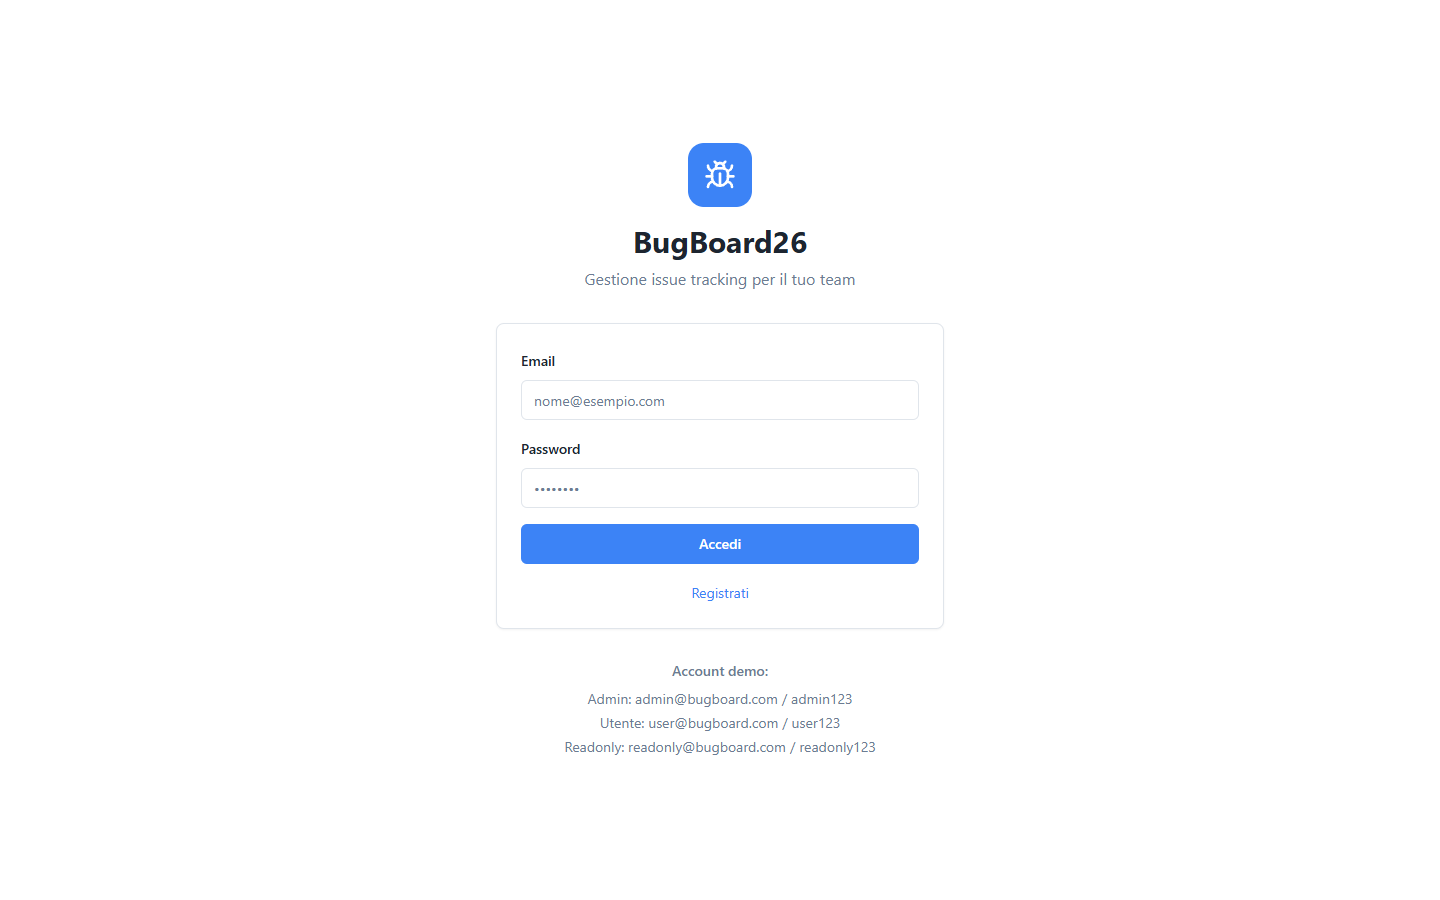
\includegraphics[width=0.85\textwidth]{immagini/mockup_01_login.png}
    \caption{Pagina di Login: form con email e password, pulsante di accesso}
    \label{fig:mockup_login}
\end{figure}

\begin{itemize}
    \item \textbf{Scopo}: autenticazione dell'utente al sistema
    \item \textbf{Elementi}: campo email, campo password, pulsante ``Accedi'', link alla pagina di registrazione
    \item \textbf{Comportamento}: in caso di credenziali errate viene mostrato un messaggio di errore inline; in caso di successo l'utente viene reindirizzato alla Dashboard
\end{itemize}

% ------- 2. REGISTRAZIONE -------
\subsubsection{Mock-up 2 --- Pagina di Registrazione}

\begin{figure}[H]
    \centering
    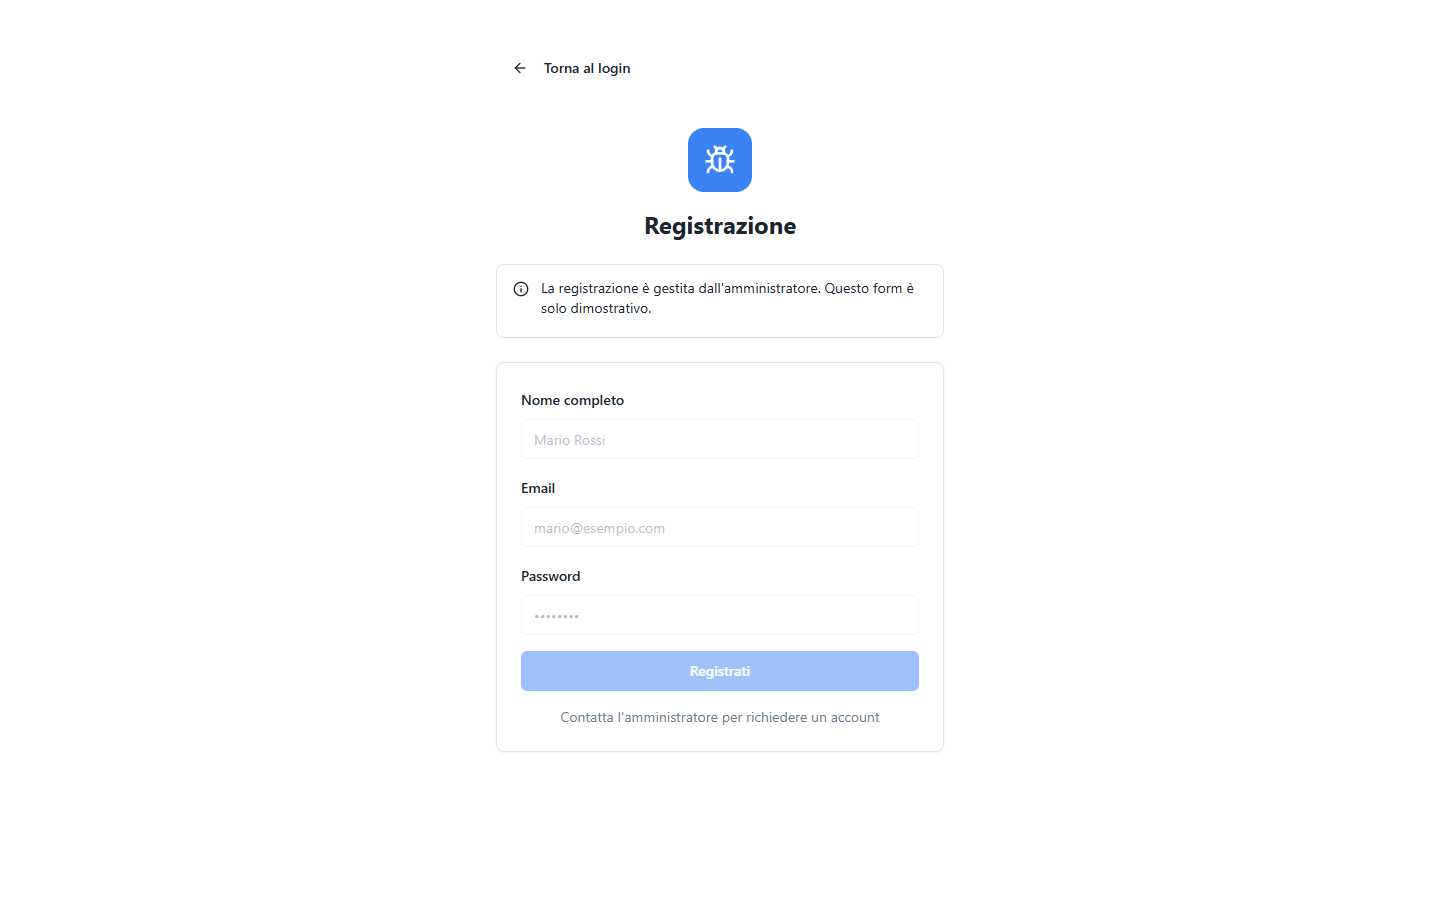
\includegraphics[width=0.85\textwidth]{immagini/mockup_02_register.png}
    \caption{Pagina di Registrazione: form con dati personali e creazione account}
    \label{fig:mockup_register}
\end{figure}

\begin{itemize}
    \item \textbf{Scopo}: creazione di un nuovo account utente
    \item \textbf{Elementi}: campi nome, email, password, conferma password; pulsante ``Registrati''
    \item \textbf{Validazione}: i campi vengono validati in tempo reale con messaggi di errore inline
\end{itemize}

% ------- 3. HOME -------
\subsubsection{Mock-up 3 --- Home / Dashboard}

\begin{figure}[H]
    \centering
    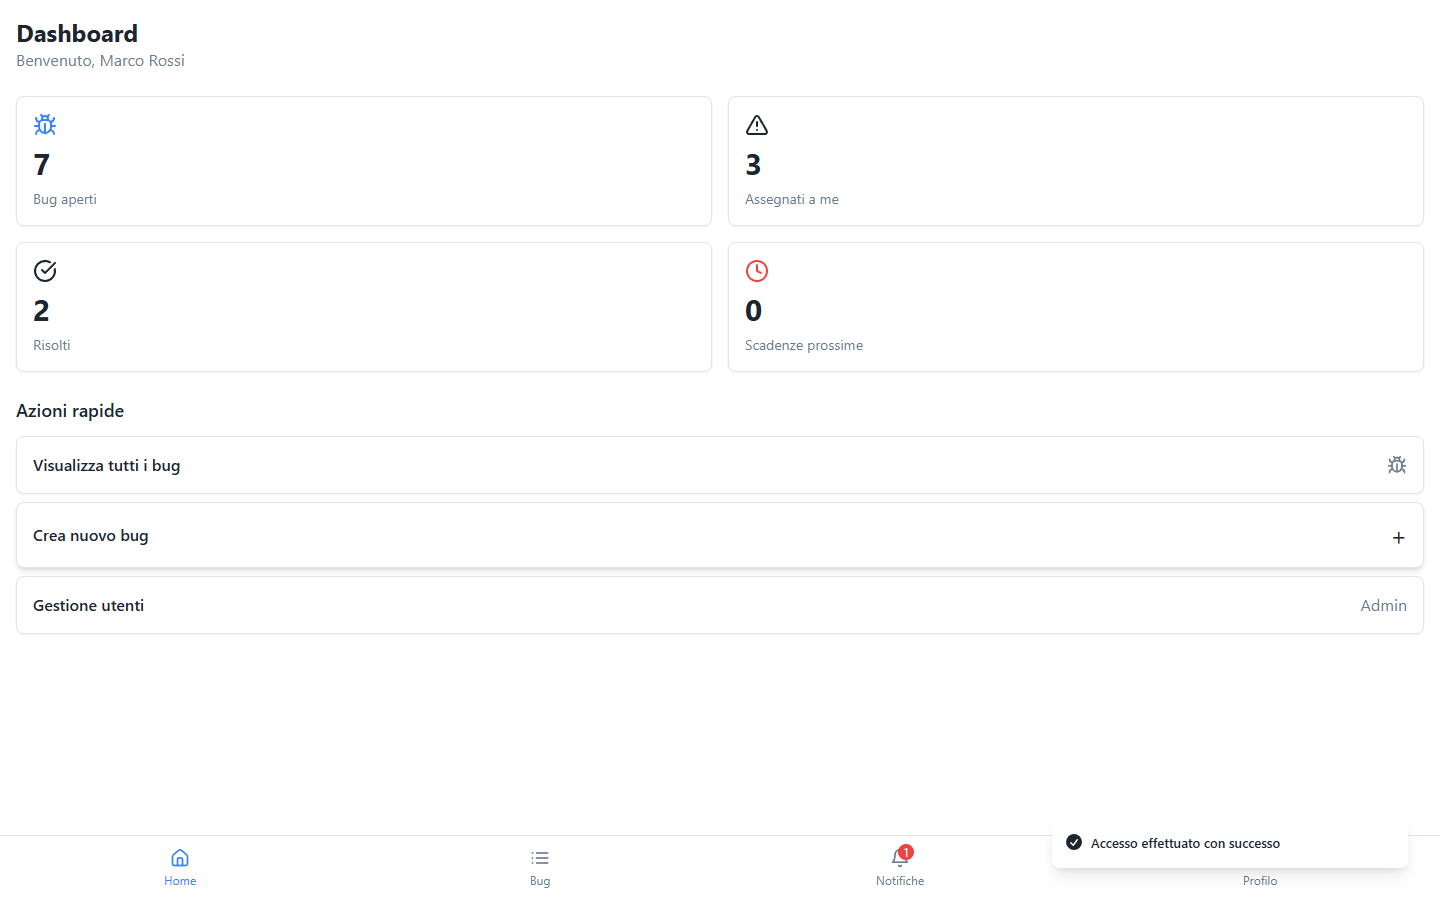
\includegraphics[width=0.85\textwidth]{immagini/mockup_03_home_dashboard.png}
    \caption{Home Dashboard: panoramica delle metriche principali e accessi rapidi}
    \label{fig:mockup_home}
\end{figure}

\begin{itemize}
    \item \textbf{Scopo}: fornire una panoramica immediata dello stato del sistema dopo il login
    \item \textbf{Elementi}: card metriche (bug aperti, assegnati a me, risolti, scadenze prossime), header con navigazione principale
    \item \textbf{Accessi rapidi}: da qui si può navigare alla lista bug, al form di creazione e ai report
\end{itemize}

% ------- 4. LISTA BUG -------
\subsubsection{Mock-up 4 --- Lista Bug con Filtri}

\begin{figure}[H]
    \centering
    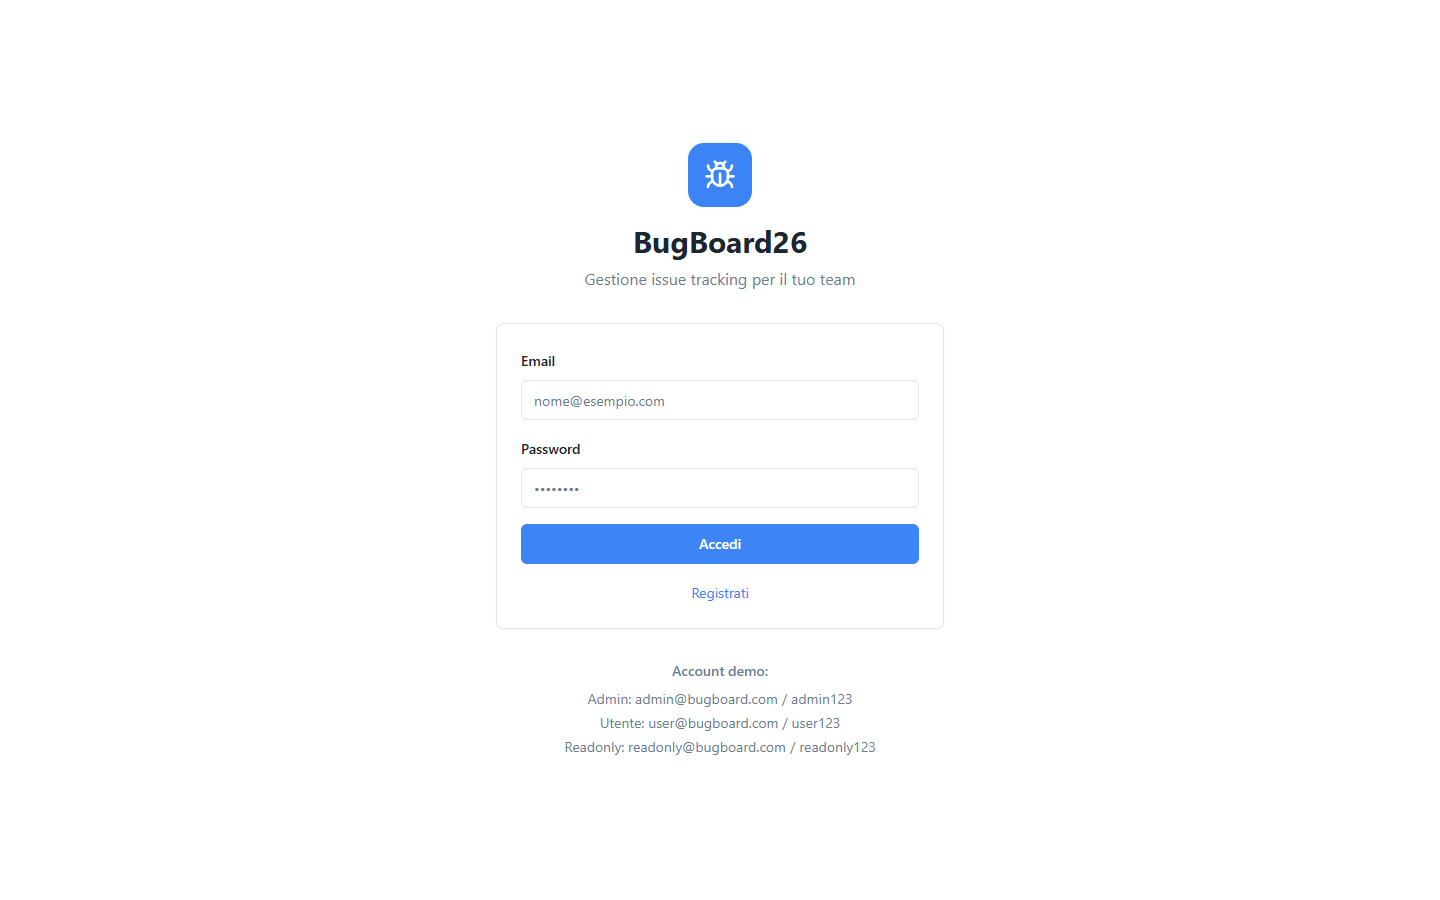
\includegraphics[width=0.85\textwidth]{immagini/mockup_04_lista_bug.png}
    \caption{Lista Bug: tabella con filtri per tipo, stato, priorità e ricerca testuale}
    \label{fig:mockup_lista_bug}
\end{figure}

\begin{itemize}
    \item \textbf{Scopo}: visualizzazione e filtraggio dell'elenco completo dei bug
    \item \textbf{Elementi}: barra filtri orizzontale (tipo, stato, priorità), campo ricerca full-text, tabella bug con badge colorati, paginazione
    \item \textbf{Interazione}: clic su una riga apre il dettaglio del bug; i filtri si applicano in tempo reale
\end{itemize}

% ------- 5. DETTAGLIO BUG -------
\subsubsection{Mock-up 5 --- Dettaglio Bug}

\begin{figure}[H]
    \centering
    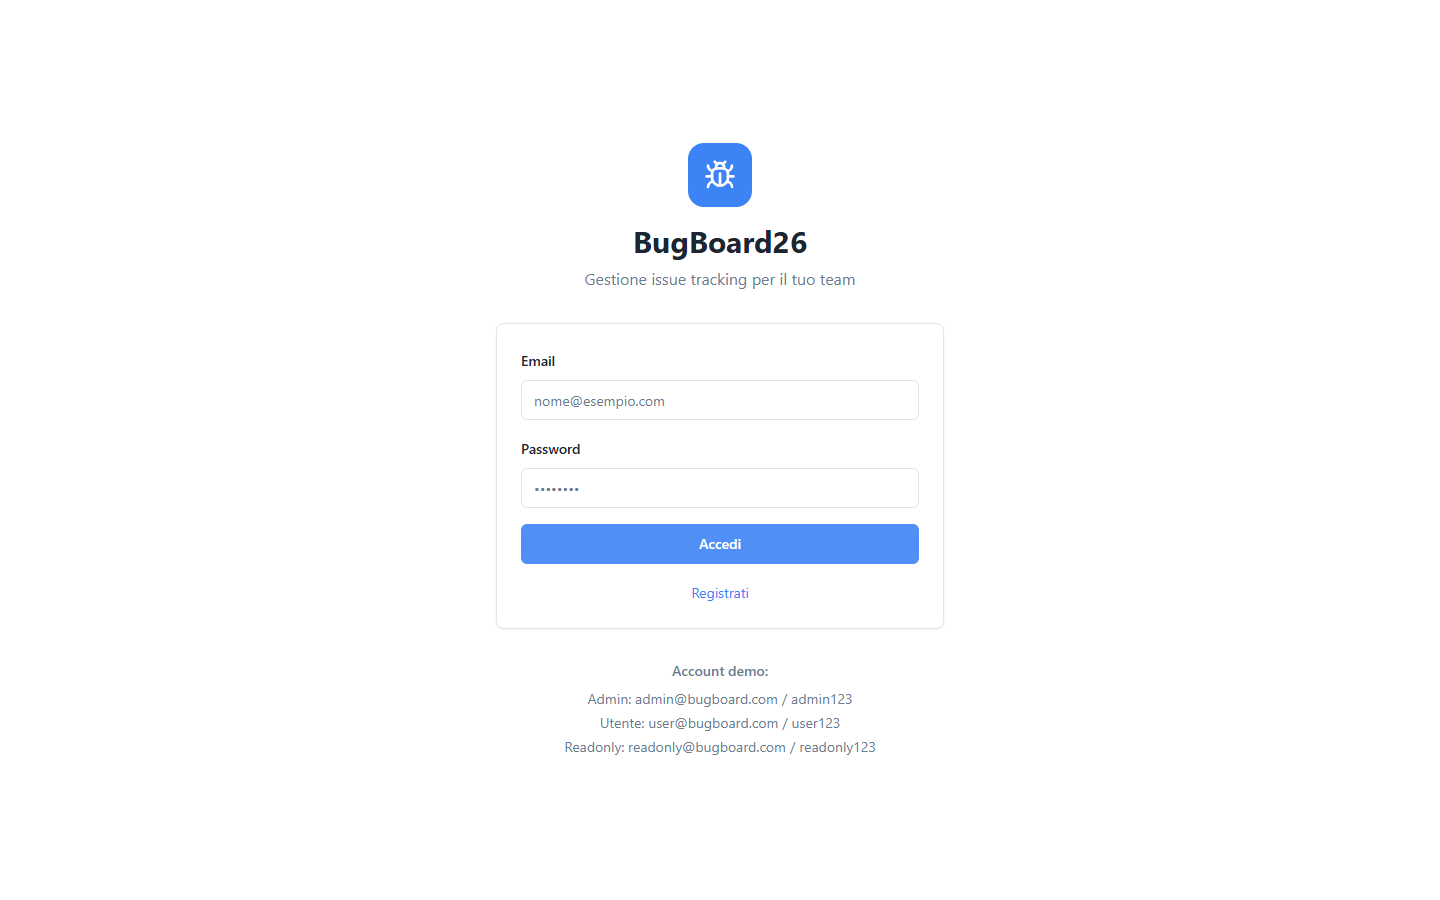
\includegraphics[width=0.85\textwidth]{immagini/mockup_05_dettaglio_bug.png}
    \caption{Dettaglio Bug: informazioni complete, commenti, storico modifiche e azioni disponibili}
    \label{fig:mockup_dettaglio_bug}
\end{figure}

\begin{itemize}
    \item \textbf{Scopo}: visualizzazione completa di un bug specifico e gestione delle azioni disponibili
    \item \textbf{Elementi}: header con titolo, stato e priorità; sezioni descrizione, commenti, allegati, storico; barra azioni laterale (modifica, assegna, risolvi, archivia, duplica)
    \item \textbf{Azioni visibili}: dipendono dal ruolo dell'utente (USER vede meno azioni rispetto ad Admin)
\end{itemize}

% ------- 6. FORM CREAZIONE BUG (UC01) -------
\subsubsection{Mock-up 6 --- Form Creazione/Modifica Bug \textbf{[UC01]}}

\begin{figure}[H]
    \centering
    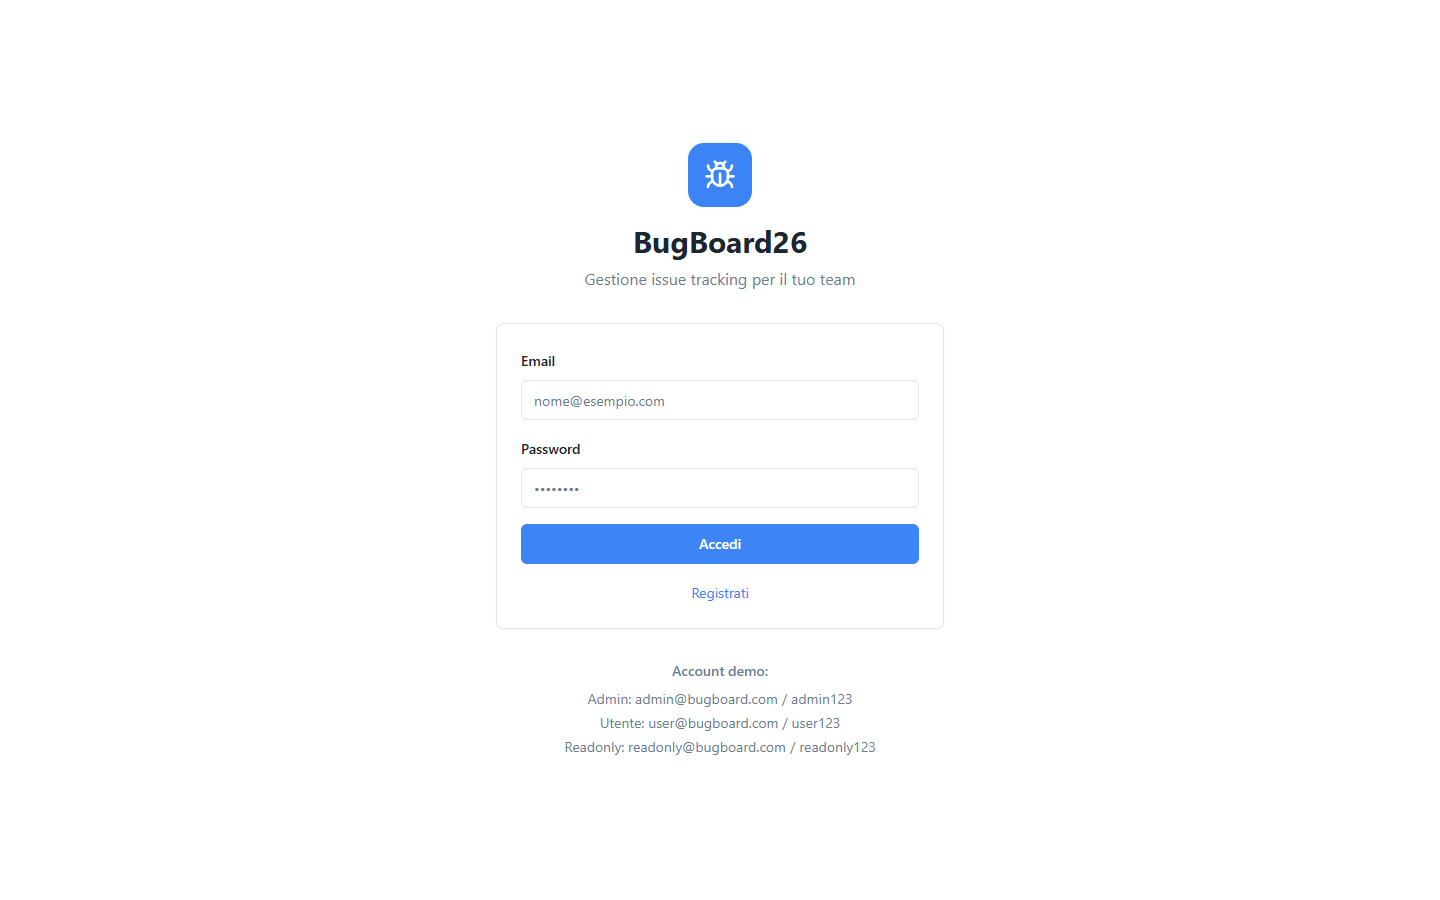
\includegraphics[width=0.85\textwidth]{immagini/mockup_06_form_creazione_bug.png}
    \caption{Form Creazione Bug (UC01): campi titolo, tipo, priorità, descrizione, label, allegati}
    \label{fig:mockup_form_bug}
\end{figure}

\begin{itemize}
    \item \textbf{Caso d'uso}: UC01 --- Creazione nuovo bug
    \item \textbf{Elementi}: campo titolo, selettori tipo e priorità, area di testo descrizione, selezione label multipla, upload allegati immagine, selezione assegnatario opzionale, pulsante ``Salva''
    \item \textbf{Validazione}: i campi obbligatori (titolo, tipo, priorità) sono evidenziati se lasciati vuoti; il formato e la dimensione degli allegati sono verificati prima dell'invio
\end{itemize}

% ------- 7. ASSEGNAZIONE BUG (UC02) -------
\subsubsection{Mock-up 7 --- Assegnazione Bug \textbf{[UC02]}}

\begin{figure}[H]
    \centering
    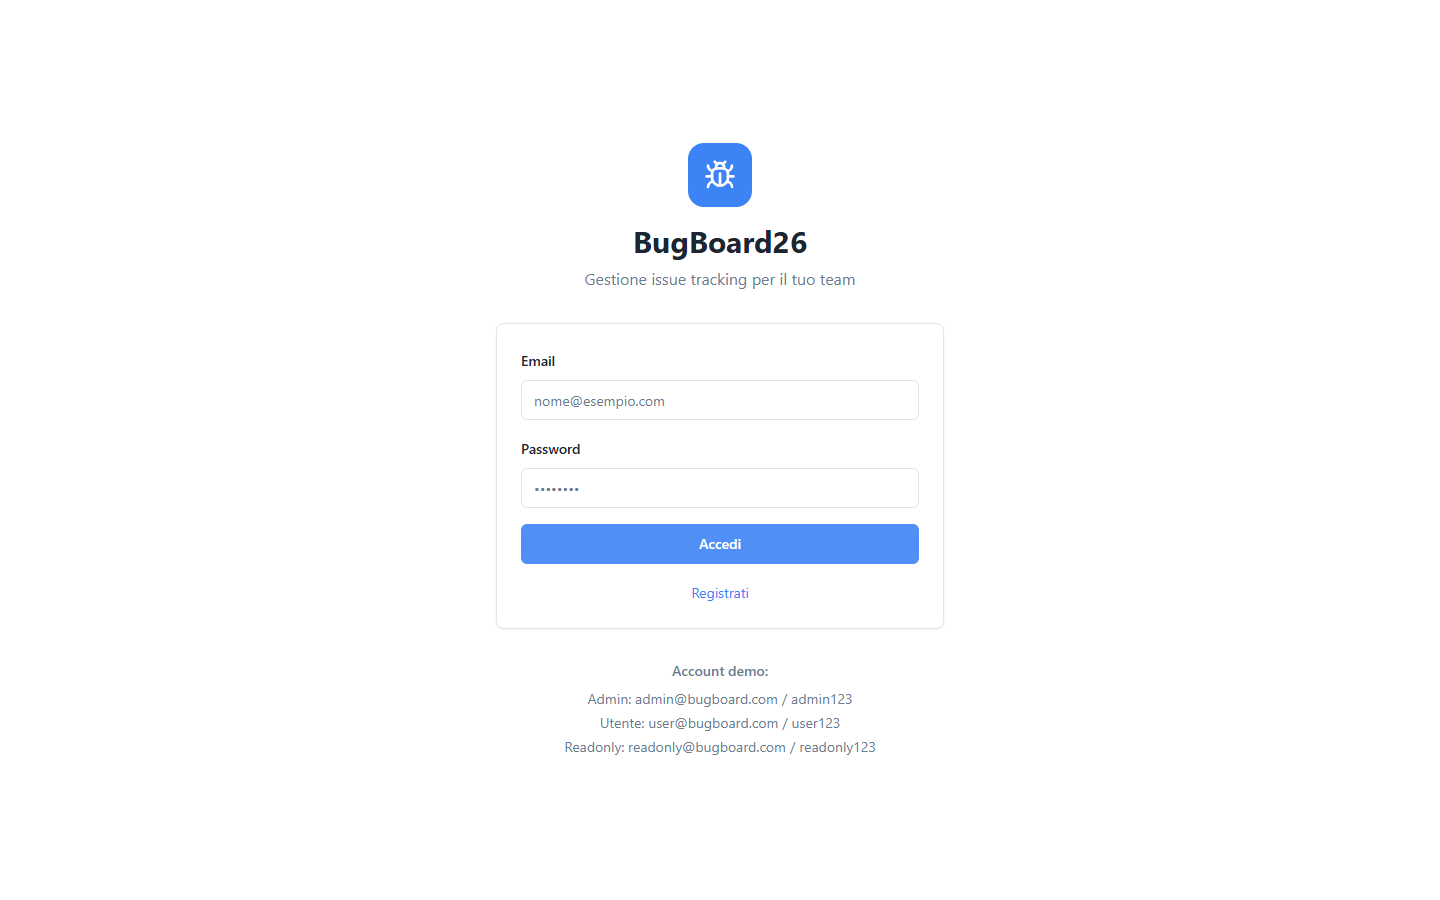
\includegraphics[width=0.85\textwidth]{immagini/mockup_07_assegnazione_bug.png}
    \caption{Assegnazione Bug (UC02): selezione dell'utente a cui assegnare il bug}
    \label{fig:mockup_assegnazione}
\end{figure}

\begin{itemize}
    \item \textbf{Caso d'uso}: UC02 --- Assegnazione bug a un utente (solo Admin)
    \item \textbf{Elementi}: select per la scelta dell'utente assegnatario, pulsante conferma
    \item \textbf{Accesso}: questa schermata è accessibile solo agli utenti con ruolo Admin; un USER viene reindirizzato alla Dashboard
\end{itemize}

% ------- 8. NOTIFICHE -------
\subsubsection{Mock-up 8 --- Notifiche}

\begin{figure}[H]
    \centering
    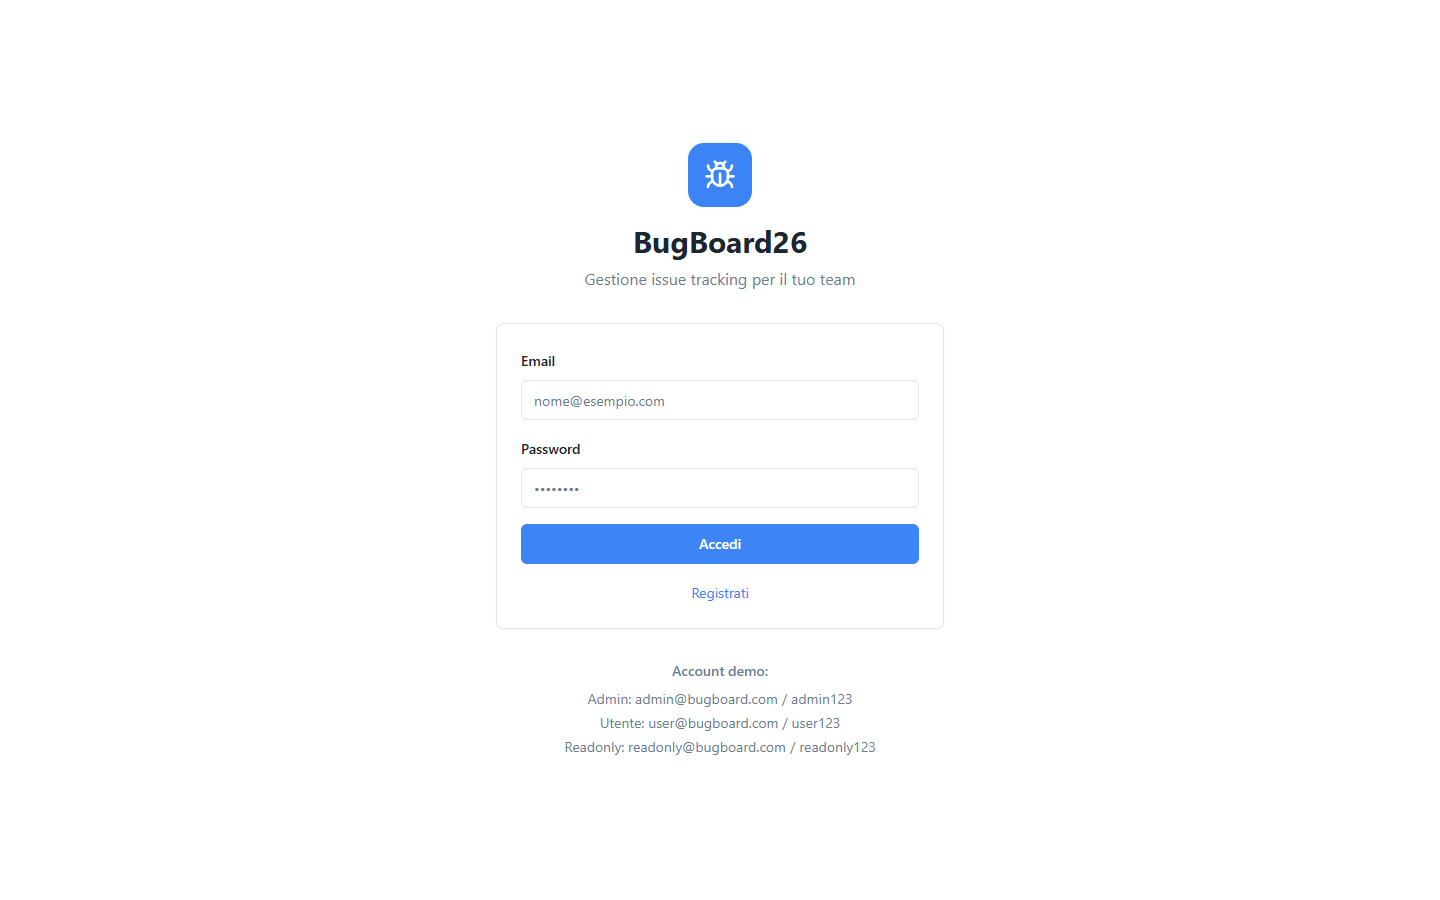
\includegraphics[width=0.85\textwidth]{immagini/mockup_08_notifiche.png}
    \caption{Centro Notifiche: lista degli aggiornamenti sui bug seguiti dall'utente}
    \label{fig:mockup_notifiche}
\end{figure}

\begin{itemize}
    \item \textbf{Scopo}: mostrare all'utente gli aggiornamenti recenti sui bug che lo riguardano (assegnazioni, cambi stato, nuovi commenti)
    \item \textbf{Elementi}: lista notifiche con timestamp, tipo evento e link al bug correlato; indicatore notifiche non lette
\end{itemize}

% ------- 9. PROFILO -------
\subsubsection{Mock-up 9 --- Profilo Utente}

\begin{figure}[H]
    \centering
    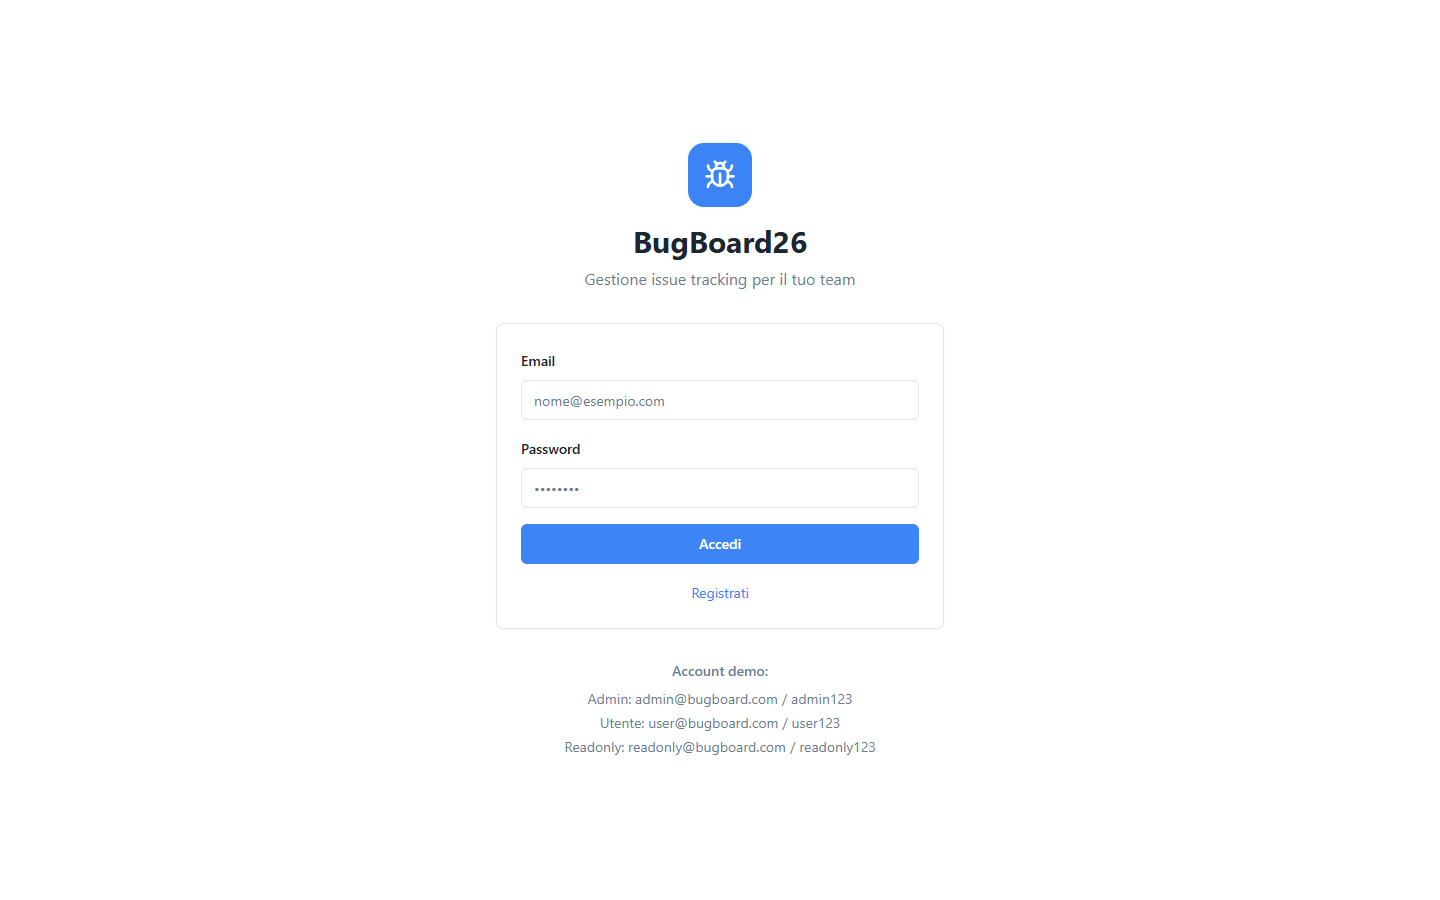
\includegraphics[width=0.85\textwidth]{immagini/mockup_09_profilo.png}
    \caption{Profilo Utente: gestione informazioni personali e cambio password}
    \label{fig:mockup_profilo}
\end{figure}

\begin{itemize}
    \item \textbf{Scopo}: consentire all'utente di visualizzare e modificare le proprie informazioni e la password
    \item \textbf{Elementi}: nome, email, ruolo (in sola lettura), form cambio password con validazione
\end{itemize}

% ------- 10. REPORT MENSILE (UC04) -------
\subsubsection{Mock-up 10 --- Report Mensile \textbf{[UC04]}}

\begin{figure}[H]
    \centering
    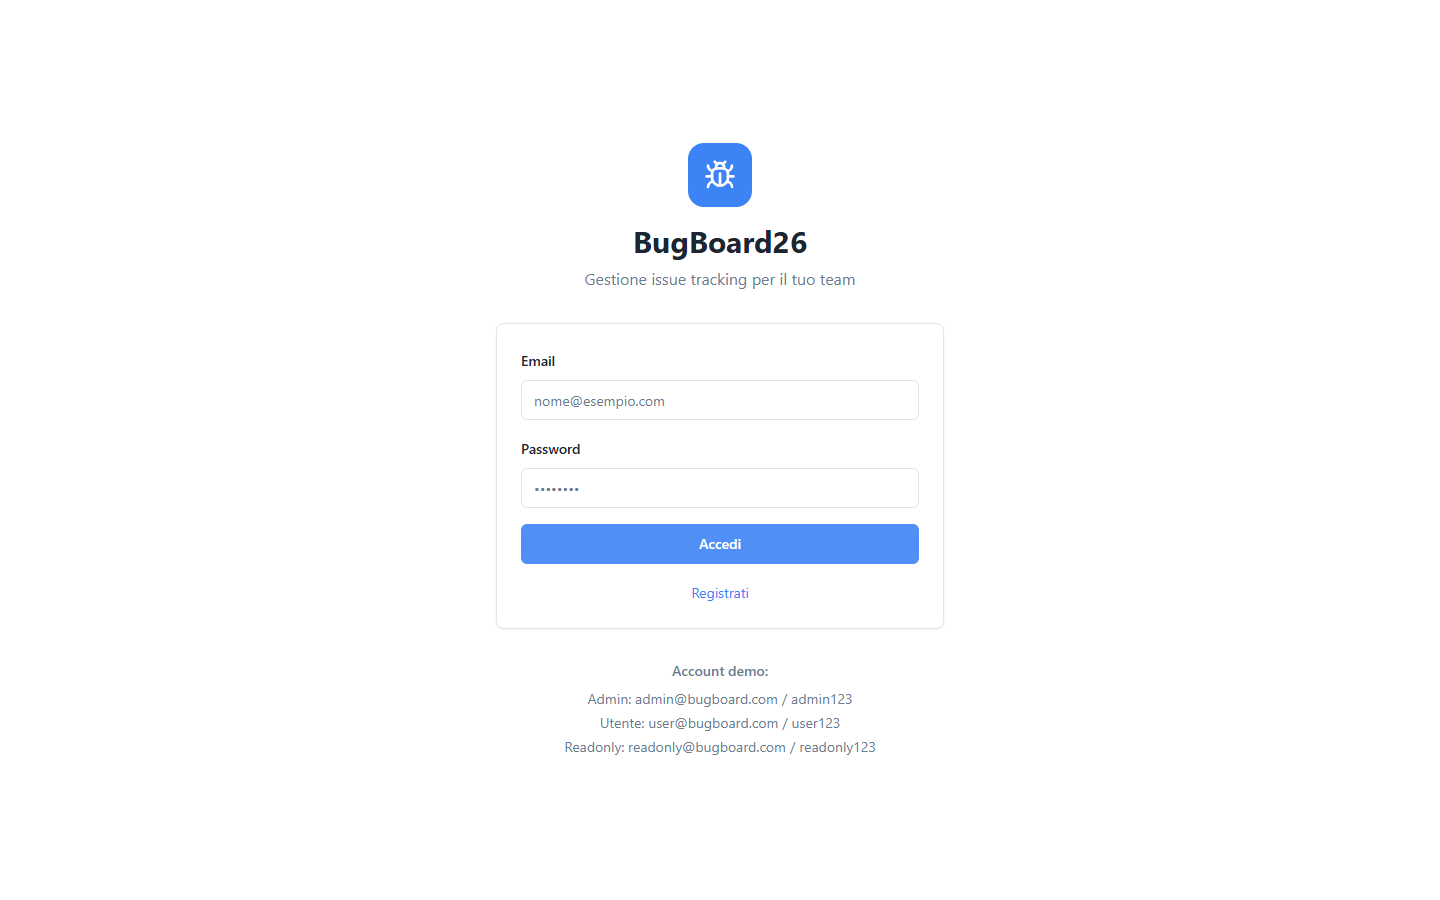
\includegraphics[width=0.85\textwidth]{immagini/mockup_10_report_mensile.png}
    \caption{Report Mensile Admin (UC04): statistiche, grafici e pulsante di export Excel}
    \label{fig:mockup_report}
\end{figure}

\begin{itemize}
    \item \textbf{Caso d'uso}: UC04 --- Generazione report mensile (solo Admin)
    \item \textbf{Elementi}: selettore mese/anno, grafici (distribuzione stato, priorità, trend temporale), tabella riassuntiva metriche, pulsante ``Esporta Excel''
    \item \textbf{Accesso}: solo Admin; gli altri utenti vengono reindirizzati alla Dashboard
\end{itemize}

% ------- 11. GESTIONE UTENTI ADMIN -------
\subsubsection{Mock-up 11 --- Gestione Utenti (Admin)}

\begin{figure}[H]
    \centering
    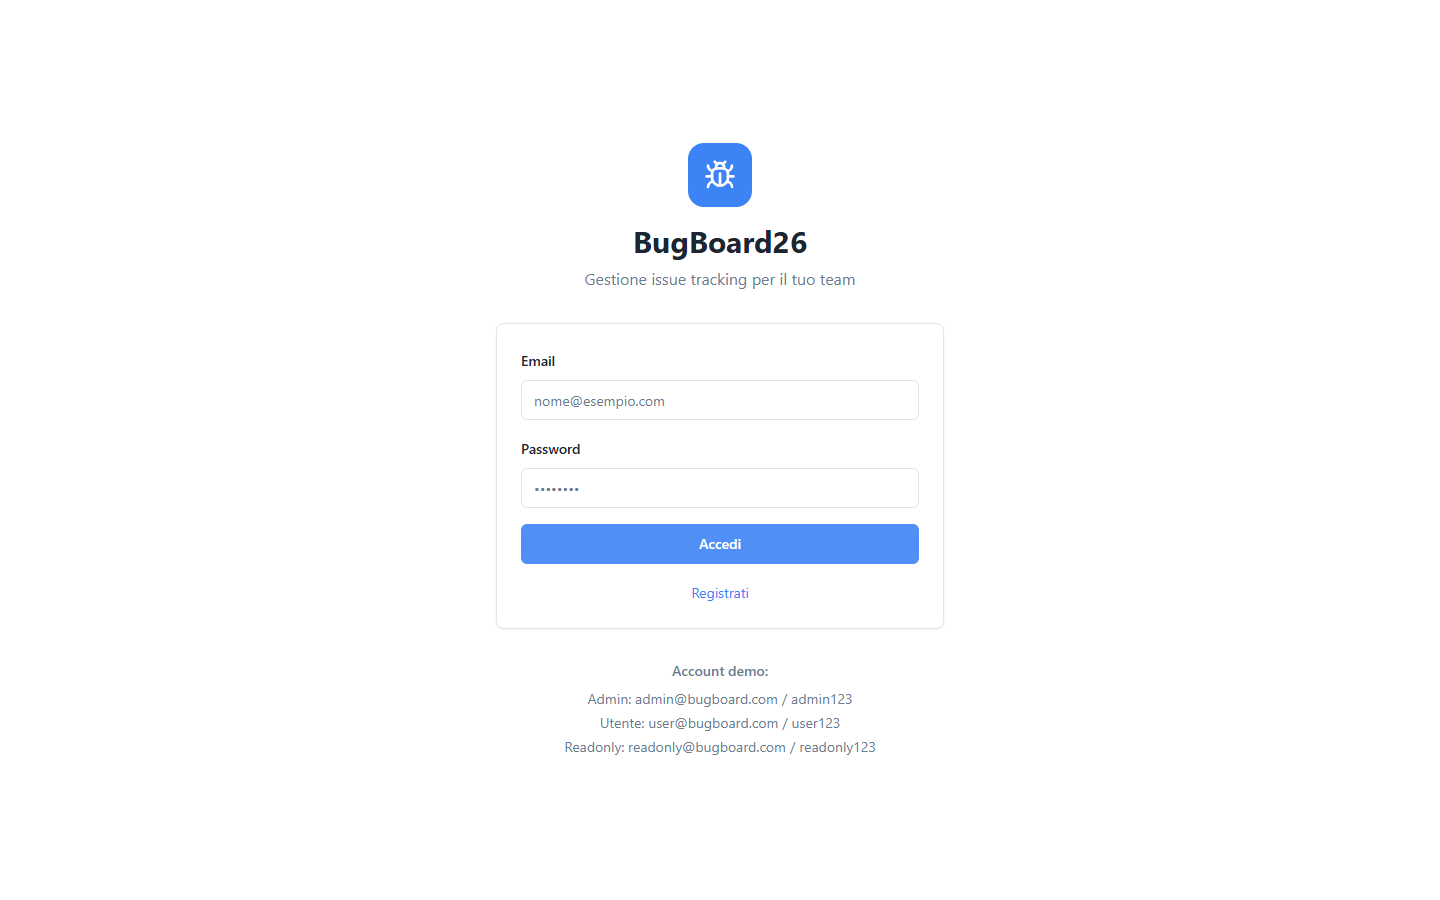
\includegraphics[width=0.85\textwidth]{immagini/mockup_11_admin_utenti.png}
    \caption{Gestione Utenti Admin: lista utenti con ruoli, stato e azioni di modifica}
    \label{fig:mockup_admin_utenti}
\end{figure}

\begin{itemize}
    \item \textbf{Scopo}: permettere all'Admin di gestire gli account del sistema (visualizzazione ruoli, disabilitazione utenti)
    \item \textbf{Elementi}: tabella utenti con email, nome, ruolo e stato; azioni per modifica ruolo e disabilitazione account
\end{itemize}

% ------- 12. ARCHIVIO -------
\subsubsection{Mock-up 12 --- Archivio Bug}

\begin{figure}[H]
    \centering
    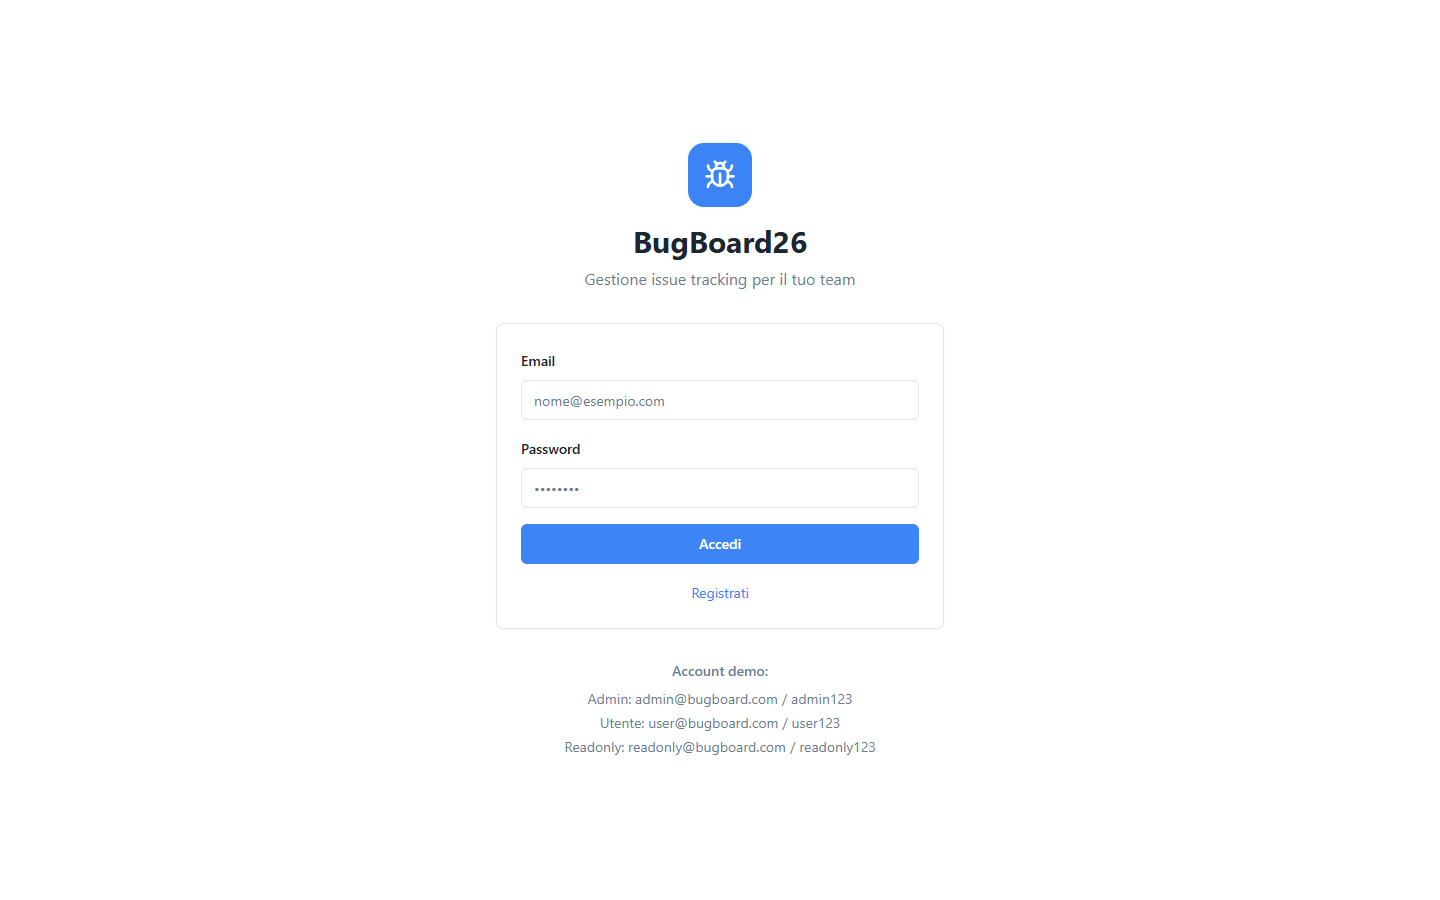
\includegraphics[width=0.85\textwidth]{immagini/mockup_12_archivio.png}
    \caption{Archivio Bug: lista dei bug archiviati con possibilità di consultazione}
    \label{fig:mockup_archivio}
\end{figure}

\begin{itemize}
    \item \textbf{Scopo}: visualizzare i bug archiviati per storico e consultazione senza influire sulla lista attiva
    \item \textbf{Elementi}: tabella bug in stato \textit{Archived} con filtri e ricerca; solo Admin può archiviare/ripristinare bug
\end{itemize}

% ------- 13. EXPORT -------
\subsubsection{Mock-up 13 --- Export Dati}

\begin{figure}[H]
    \centering
    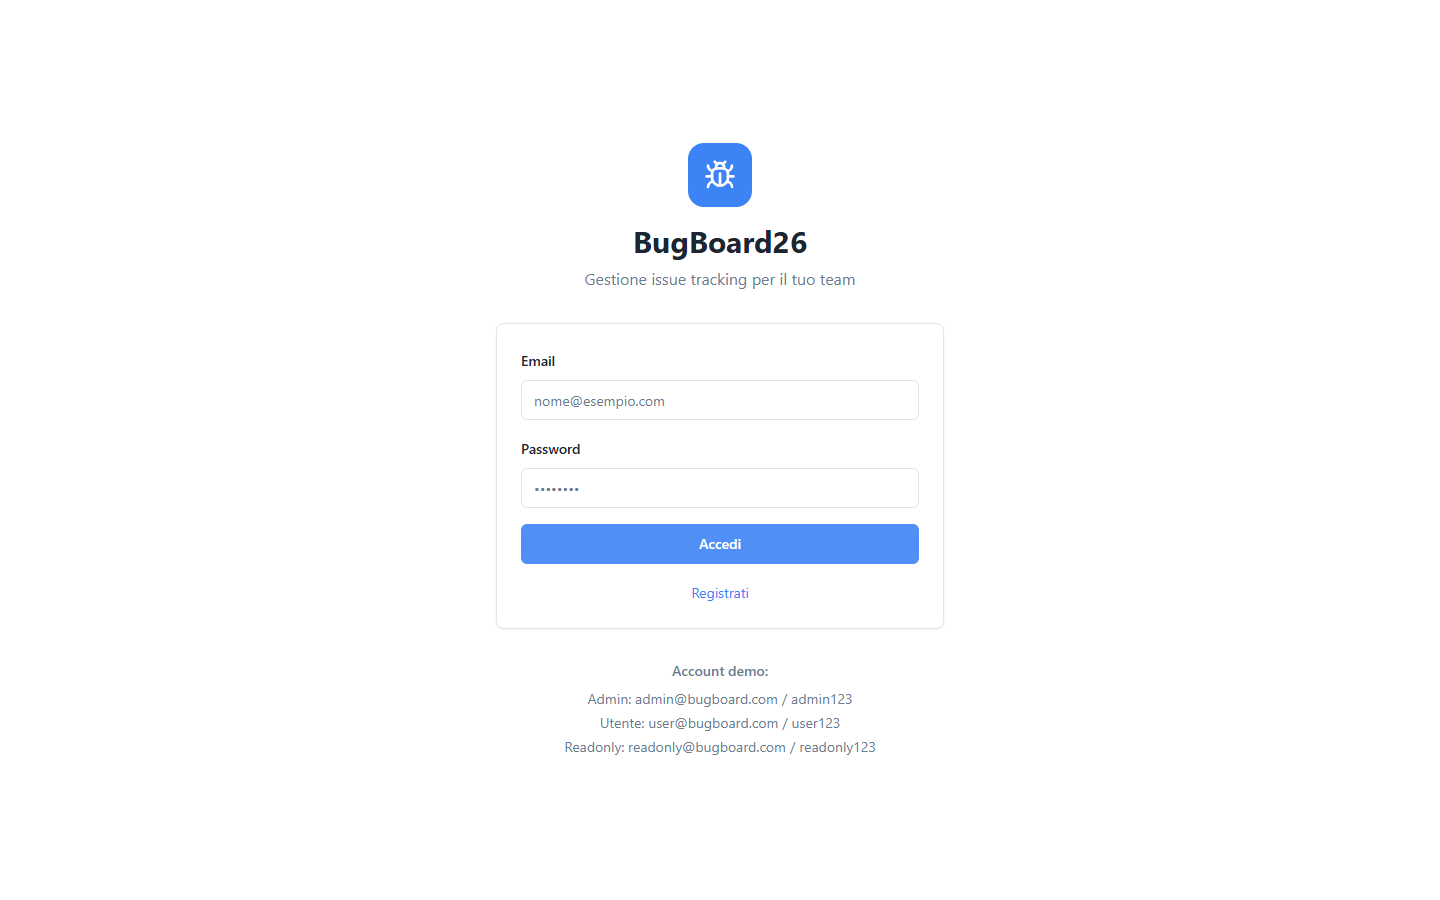
\includegraphics[width=0.85\textwidth]{immagini/mockup_13_export.png}
    \caption{Export Dati: download dell'elenco bug in formato CSV o Excel}
    \label{fig:mockup_export}
\end{figure}

\begin{itemize}
    \item \textbf{Scopo}: consentire l'esportazione dei dati per analisi esterne
    \item \textbf{Elementi}: pulsanti ``Scarica CSV'' e ``Scarica Excel''; i file vengono generati dal backend e scaricati direttamente
\end{itemize}

% ------------------------------------------------------------
\subsection{Osservazioni emerse dalla prototipazione}

La realizzazione del prototipo funzionante ha permesso di identificare alcune scelte migliorative rispetto all'analisi iniziale:

\begin{itemize}
    \item \textbf{Chiarezza dei ruoli}: è stato necessario rendere esplicito nel UI quali azioni sono riservate all'Admin (assegnazione, report, archiviazione, gestione utenti), aggiungendo reindirizzamenti automatici per utenti non autorizzati
    \item \textbf{Filtri immediati}: la lista bug con filtri in tempo reale si è rivelata la funzionalità più usata nelle sessioni di test, confermando la scelta di renderla la pagina principale
    \item \textbf{Badge colorati}: l'uso di badge cromatici per stato, priorità e tipo ha migliorato significativamente la leggibilità della lista bug senza aprire il dettaglio
    \item \textbf{Navigazione mobile}: il menu hamburger con le stesse voci del desktop ha garantito piena parità funzionale su dispositivi mobili
\end{itemize}
